\chapter{Searches for Heavy Stable Charged Particles \label{sec:search}}

\section{Introduction}
As discussed in section~\ref{sec:BSM}, new heavy long-lived charged particles are predicted in many extensions to the SM. HSCPs with
lifetimes $\gtrsim 40$~ns are likely to traverse the entire CMS detector before decaying and will thus be directly detectable.
Some of the HSCP combine with SM particles to form composite objects that can be electrically charged or neutral.
Interactions with the CMS detector may change the SM constituents of the particles and through this their electric charge.
The HSCPs will be produced with high momentum but their large mass means that
a majority will have a velocity, $\beta \equiv v/c,$ less than 0.9.
As no heavy long-lived SM particles are expected to be produced at the LHC, HSCPs would be the only high-momentum particles with $\beta$ not very close to one.
Detector signatures unique to slow-moving particles are exploited to search for HSCP.
The backgrounds to the searches are SM particles with detector mismeasurement and in some cases
muons coming from cosmic rays. This chapter details multiple searches for HSCP.

The contents of this chapter are included in a paper authored by the CMS collaboration~\cite{Chatrchyan:2013oca}.
The work was done in a small group within the CMS collaboration with me being one of the central analyzers.
Other major contributors to the work were Loic Quertenmont, Todd Adams, Giacomo Bruno, Jie Chen, Venkatesh Veeraraghavan, and Wells Wulsin.
The paper includes five searches for HSCPs in data collected by CMS during 2011 running at $\sqrt{s}=7$~TeV and 2012 running at 8~TeV.
Each search is designed to have sensitivity for various different signatures of HSCP. 
The five searches are all done in the same framework,
so most of my work was applied to all five analyses. The five searches are labelled \muononly, \tktof, \tkonly, \multi, and \fract. 

The \muononly\ analysis requires only that a track be found in the muon system of CMS.
This analysis is expected to still have sensitivity when all particles are produced electrically neutral. The
\tktof\ analysis requires that the muon system track be matched to a track in the inner tracker. This analysis is especially
powerful for lepton-like HSCP. The third analysis is the \tkonly\ analysis that only requires a track be found in the inner tracker so that it can be sensitive to particles
becoming neutral in the calorimeter and leaving no hits in the muon system. The \multi\ analysis looks 
for particles with $Q > 1e$ and reconstructed like in the \tktof\ analysis. The \fract\ analysis searches for particles with $Q < 1e$ and only
requires the particles to be found in the inner tracker.

For parts of the searches that were different between the five searches,
I was essentially the only person to work on the \muononly\ search and contributed largely to the \tktof\ search.
I worked on the \tkonly\ and \multi\ searches to a slightly smaller degree. My work on the \fract\ search was mostly limited those aspects 
that were applied across all five searches. 
Therefore this chapter mostly focuses on the \muononly\ and \tktof\ searches, while the \tkonly\ and \multi\ searches are presented
with the specific parts that I worked on highlighted. The \fract\ search is not presented here.

The CMS paper includes both the 2011 and 2012 data taking periods for all the analyses except for the \muononly\ search which uses the 2012 data only. 
As the \muononly\ search is the major focus of this chapter, it was decided to focus on the data collected in 2012 for this chapter.
Additionally, the 2012 dataset was taken at a higher energy and includes approximately four times the integrated luminosity as the 2011 dataset,
making the sensitivity of the searches determined to a large degree by the data collected in 2012.
The procedure for analyzing the data from the two periods is identical.
A statistical combination of the 2011 and 2012 dataset for all the analyses except for \muononly\ is presented at the end of the chapter. 

Previous collider searches for HSCPs have been performed at LEP~\cite{Barate:1997dr, Abreu:2000tn, Achard:2001qw, Abbiendi:2003yd}, HERA~\cite{Aktas:2004pq},
the Tevatron~\cite{Abazov:2008qu, Aaltonen:2009kea, Abazov:2011pf,Abazov:2012ab},
and the LHC~\cite{Khachatryan:2011ts, Aad:2011mb,  Aad:2011yf, Aad:2011hz, CMS:2012xi, Chatrchyan:2012sp, Aad:2012vd, Aad:2013pqd}.
The results from such searches have placed important bounds on BSM theories~\cite{Berger:2008cq, CahillRowley:2012kx}. 
The most stringent limits have come from previous LHC searches that placed limits on the mass of gluinos, stops, and staus at 1098,
737, and 223 GeV/$c^2$~\cite{Chatrchyan:2012sp}, respectively.

For all plots in this chapter, the first and last bins contain the underflow and overflow, respectively.

\section{Samples \label{sec:samples}}

Data collected with the CMS detector during 2012 running at an energy of $\sqrt{s}=8$~TeV are searched. The data collection was split into four periods labeled A, B, C, and D.
All data collected by CMS undergo a prompt reconstruction as described in section~\ref{sec:computing}. The first two run periods, A and B, underwent an additional
re-reconstruction so as to have the latest reconstruction improvements and calibration constants. The re-reconstructed samples are used for the A and B periods while the promptly
reconstructed samples are used for the C and D periods.

CMS has a Data Certification team which checks all data collected and certifies the data as good for analysis. The certification requires all detector subsystems to be
operating at full ability, or at least close enough to full ability to not have a detrimental effect on offline analyses. Additionally, higher level objects such as muons
and electrons are checked to make sure the data are good for physics analyses. For this particular analysis, the RPC trigger plays an important role, as discussed in
section~\ref{sec:trigger}, and so the RPC is required to be included in the L1 trigger for all data searched. This leads to the searches using slightly less data
than most other CMS analyses on 2012 data. The data sample used by this analysis corresponds to 18.8~fb$^{-1}$.

Multiple different signal Monte Carlo (MC) simulation samples are produced to account for the different signatures an HSCP could have;
more detail on the signal models can be found in Sec.~\ref{sec:BSM}.

Pair production of strongly--interacting gluino and stop samples are produced with
masses in the range 300--1500~GeV$/c^2$ and 100--1000~GeV$/c^2$, respectively.
The gluinos are generated in the split SUSY scenario~\cite{ArkaniHamed:2004fb, Giudice:2004tc}. 
under the assumption of high squark masses of 10~TeV. The samples are generated using PYTHIAv8.153~\cite{Sjostrand:2007gs}
Samples are produced with the fraction $f$ of gluinos forming neutral glueball $R-hadrons$ set to $f=1.0$, 0.5, and 0.1.
%The value of $f=1.0$ results in all gluino $R-hadrons$ being produced neutral.
%, the \muononly\ analysis is designed to still have sensitivity in this case.
The samples are also produced with two different modelings of the nuclear interaction of R-hadrons with matter: the cloud interaction and charge suppressed models.
The charge suppressed model results in all $R-hadrons$ being neutral after a nuclear interaction.
The cloud interaction model should be assumed for samples unless explicitly stated otherwise.
Most HSCP will not have a nuclear interaction while passing through the CMS tracker, however almost all of them will have such an interaction in the calorimeter.

The above effects can lead to many interesting signatures in the CMS detector. R-hadrons neutral after hadronization will generally remain neutral through the tracker
but may gain charge in the calorimeter under the cloud model and leave hits in the muon system. If the glueball fraction is 1.0, then this would
be the only way to detect gluino HSCP. The \muononly\ analysis is designed to have sensitivity to HSCP of this type. On the other hand HSCP produced charged under
the charge suppression model will likely be charged in the tracker but always neutral in the muon system. The \tkonly\ analysis is designed to be sensitive
to HSCP of this type. A third signature is an HSCP charged in both the muon and tracker systems which would have a signature similar to a muon.
HSCP produced neutral under the charge suppression model would never be charged during their passage through CMS and thus are outside the scope
of an HSCP search.%, they would fall into searches for dark matter.

The \pt, $\eta$, and $\beta$ distributions of gluino and stop particles at generation are shown in Figs.~\ref{fig:GenGluino} and~\ref{fig:GenStop}, respectively.

\begin{figure}
 \begin{center}
  \includegraphics[clip=false, trim=0.0cm 0cm 1.4cm 0cm, width=0.44\textwidth]{figures/muonly/Selection_Comp_GenGluino_genpT}
  \includegraphics[clip=false, trim=0.0cm 0cm 1.4cm 0cm, width=0.44\textwidth]{figures/muonly/Selection_Comp_GenGluino_geneta}
  \includegraphics[clip=false, trim=0.0cm 0cm 1.4cm 0cm, width=0.44\textwidth]{figures/muonly/Selection_Comp_GenGluino_genbeta}
 \end{center}
 \caption[Distribution of \pt, $\eta$, and $\beta$ for various gluino samples at generation]
{Distribution of various kinematic variables for various gluino ($\tilde{g}$) samples at generation:
\pt\ (top left), $\eta$ (top right), and $\beta$ (bottom).
   \label{fig:GenGluino}}
\end{figure}

\begin{figure}
 \begin{center}
  \includegraphics[clip=false, trim=0.0cm 0cm 1.4cm 0cm, width=0.44\textwidth]{figures/muonly/Selection_Comp_GenStop_genpT}
  \includegraphics[clip=false, trim=0.0cm 0cm 1.4cm 0cm, width=0.44\textwidth]{figures/muonly/Selection_Comp_GenStop_geneta}
  \includegraphics[clip=false, trim=0.0cm 0cm 1.4cm 0cm, width=0.44\textwidth]{figures/muonly/Selection_Comp_GenStop_genbeta}
 \end{center}
 \caption[Distribution of \pt, $\eta$, and $\beta$ for various stop ($\tilde{t}$) samples at generation]
{Distribution of various kinematic variables for various stop samples at generation:
\pt\ (top left), $\eta$ (top right), and $\beta$ (bottom).
   \label{fig:GenStop}}
\end{figure}

%One example of this is a neutral R-meson
%made of a a gluino, a down quark, and a down anti-quark interacting with a proton, which is composed of two up quarks

Additional samples are produced creating lepton-like HSCP. Stau pair samples
are produced under the minimal gauge-mediated supersymmetry breaking (mGMSB) scenario~\cite{Giudice:1998bp} using the SPS7 slope~\cite{Allanach:2002nj}.
The ISASUGRA version 7.69~\cite{Paige:2003mg} program is used to set the particle mass scale and decay chains by specifying six parameters.
%Six parameters are set to specify the exact mGMSB scenario used. 
The number of messenger particles is set to three; the ratio of the mass of the messenger particles to the effective SUSY breaking mass scale is set to two;
$tan \beta = 10$, this $\beta$ being the ratio of the vacuum expectation values of the neutral Higgses;
the sign of the supersymmetric Higgs mass parameter is made greater than zero; and $c_{Grav}$ is greater than 10000.
The low number of messenger particles results in the stau being the NLSP.
The high value of $C_{Grav}$ results in the stau being long-lived while varying $\Lambda$ from 31 to 180~TeV gives staus within a mass range of 100--557~GeV$/c^2$. 
The produced mass spectrum and decay chains are passed to PYTHIAv6.426~\cite{Sjostrand:2006za}. 
Stau production proceeds either by direct electroweak production or from the cascade
decay of other particles (usually through the pair production of gluinos and squarks). Cascade decay is dominant due to the strong nature of the production mechanism.
In order to give the best results while maintaining model independence, two stau samples are used: one with both direct production and production from cascade decays (CD)
and one with staus only produced through direct production (DP). The second sample is less dependent on the model parameters. The distribution of \pt, $\eta$, and $\beta$ at generation
are shown in Figs~\ref{fig:GenGMStau} and~\ref{fig:GenPPStau} for various CD and DP stau samples, respectively.

\begin{figure}
 \begin{center}
  \includegraphics[clip=false, trim=0.0cm 0cm 1.4cm 0cm, width=0.44\textwidth]{figures/muonly/Selection_Comp_GenGMStau_genpT}
  \includegraphics[clip=false, trim=0.0cm 0cm 1.4cm 0cm, width=0.44\textwidth]{figures/muonly/Selection_Comp_GenGMStau_geneta}
  \includegraphics[clip=false, trim=0.0cm 0cm 1.4cm 0cm, width=0.44\textwidth]{figures/muonly/Selection_Comp_GenGMStau_genbeta}
 \end{center}
 \caption[Distribution of \pt, $\eta$, and $\beta$ for various CD stau samples at generation]
{Distribution of various kinematic variables for various CD stau ($\tilde{\tau}$) samples at generation:
\pt\ (top left), $\eta$ (top right), and $\beta$ (bottom)
   \label{fig:GenGMStau}}
\end{figure}

\begin{figure}
 \begin{center}
  \includegraphics[clip=false, trim=0.0cm 0cm 1.4cm 0cm, width=0.44\textwidth]{figures/muonly/Selection_Comp_GenPPStau_genpT}
  \includegraphics[clip=false, trim=0.0cm 0cm 1.4cm 0cm, width=0.44\textwidth]{figures/muonly/Selection_Comp_GenPPStau_geneta}
  \includegraphics[clip=false, trim=0.0cm 0cm 1.4cm 0cm, width=0.44\textwidth]{figures/muonly/Selection_Comp_GenPPStau_genbeta}
 \end{center}
 \caption[Distribution of \pt, $\eta$, and $\beta$ for various DP stau samples at generation]
{Distribution of various kinematic variables for various DP stau ($\tilde{\tau}$) samples at generation:
\pt\ (top left), $\eta$ (top right) and $\beta$ (bottom).
   \label{fig:GenPPStau}}
\end{figure}

The last of the signal samples used is modified Drell-Yan production of long-lived leptons with different electrical charges.
In the model considered, the particles are neutral under $SU(3)_C$ and $SU(2)_L$ but still interact through $U(1)_Y$ interactions~\cite{Langacker:2011db}.
As all SM particles that reach CMS have Q equal to $1e$ or
are neutral, the possibility of HSCPs with non-unit charge is interesting. 
%Here and in the rest of this work, Q is meant to be the absolute value of the charge unless explicitly stated.
%The particles can generically be divided by whether they have Q<1e or Q>=1e.
The production of these particles is simulated with PYTHIAv6.426~\cite{Sjostrand:2006za}. 
Samples are produced with charge Q = $1e$, $2e$, $3e$, $4e$, $5e$, $6e$, $7e$, and $8e$ for masses of 
%100-500 GeV$/c^2$ for $Q=2e/3$;
100-1000~GeV$/c^2$ for $1e <= Q <= 5e$ and 200-1000~GeV$/c^2$ for $Q > 5e$.
%charge Q = 1/3, 2/3, 1, 2, 3, 4, 5, 6, 7, and 8e for masses of 100-500 GeV$/c^2$ for Q<1e, 100-1000 GeV$/c^2$ for 1e <= Q <= 5e, and 200-1000 for Q > 5e. 
%The samples can generically be divided by whether they have Q<1e or Q>=1e.
The distribution of \pt, $\eta$, and $\beta$ at generation for various charges and masses are shown in Fig.~\ref{fig:GenDY}.

\begin{figure}
 \begin{center}
  \includegraphics[clip=false, trim=0.0cm 0cm 1.4cm 0cm, width=0.44\textwidth]{figures/muonly/Selection_Comp_GenDY_genpT}
  \includegraphics[clip=false, trim=0.0cm 0cm 1.4cm 0cm, width=0.44\textwidth]{figures/muonly/Selection_Comp_GenDY_geneta}
  \includegraphics[clip=false, trim=0.0cm 0cm 1.4cm 0cm, width=0.44\textwidth]{figures/muonly/Selection_Comp_GenDY_genbeta}
 \end{center}
 \caption[Distribution of \pt, $\eta$, and $\beta$ for modified DY samples with various charges and masses at generation]
{Distribution of various kinematic for modified DY samples with various charges and masses at generation.
Top: \pt\ (left) and $\eta$ (right).
Bottom: $\beta$}
   \label{fig:GenDY}
\end{figure}

All MC simulation events are overlaid with additional proton-proton collisions, see Section~\ref{sec:LHC}.
Weights are given to the events so that the distribution of additional collisions in the MC simulation samples matches what is observed in data.
The reconstruction of the event by CMSSW tries to identify each proton-proton collision as a separate primary vertex~\cite{2010EPJC...70.1165K}.
The distribution of the number of primary vertices found in events after the reweighting is shown in Figure~\ref{fig:PV} for data and MC simulation.
The samples shown in the figure are required to have been collected with one of the triggers detailed in Sec.~\ref{sec:trigger}.

\begin{figure}
  \begin{center}
      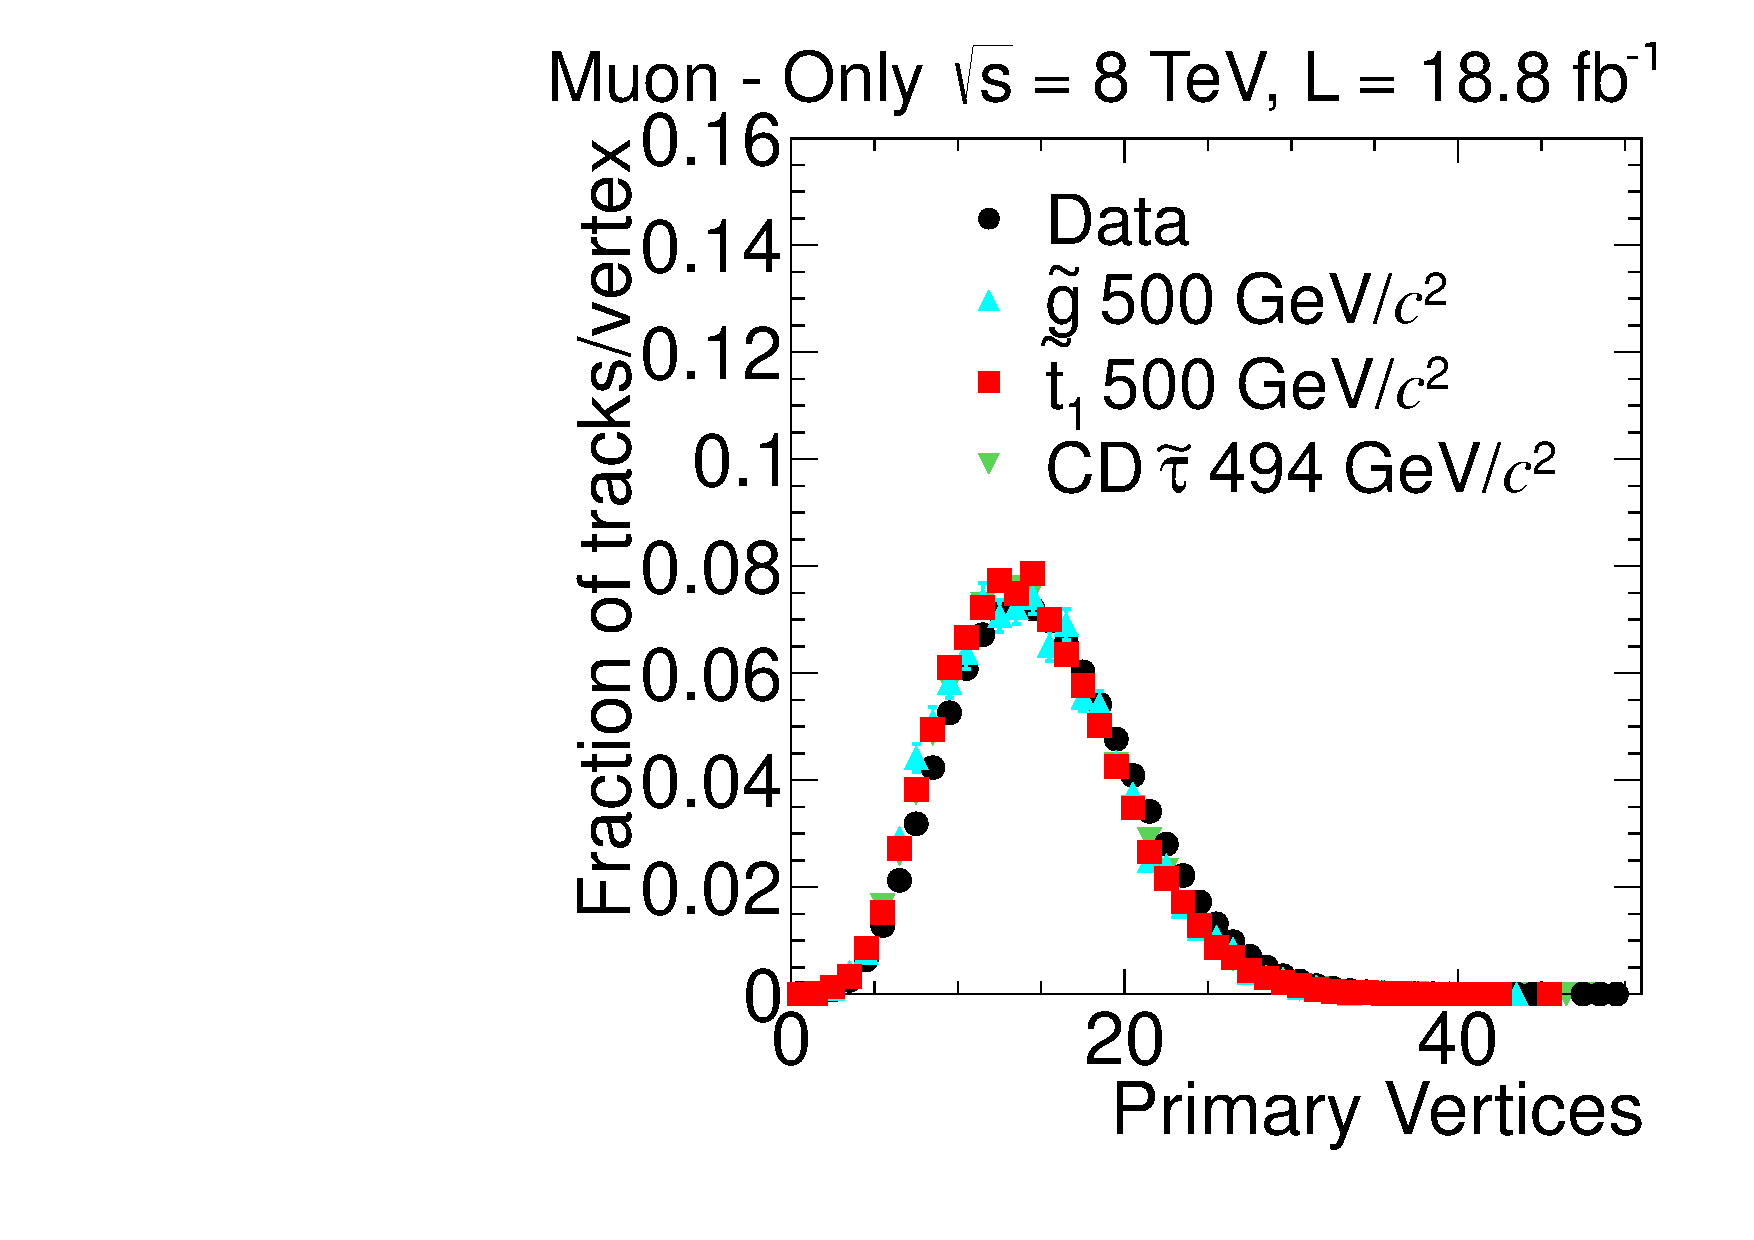
\includegraphics[clip=false, trim=0.0cm 0cm 0.0cm 0cm, width=0.44\textwidth]{figures/muonly/Selection_Comp_Signal_8TeV_PV_BS}
      \includegraphics[clip=false, trim=0.0cm 0cm 0.0cm 0cm, width=0.44\textwidth]{figures/muonly/Selection_Comp_Signal_8TeV_PVLog_BS} \\
  \end{center}
        \caption[Distribution of number of primary vertices in data and various MC simulation samples]
{Distribution of number of primary vertices in data and various MC simulation samples. 
The samples shown in the figure are required to have been collected with one of the three triggers detailed in Sec.~\ref{sec:trigger}.
Left with linear y-axis scale, right with log scale.
        }
      \label{fig:PV}
\end{figure}

\section{Trigger \label{sec:trigger}}
As discussed in Sec.~\ref{sec:computing}, in order for an event to be triggered for readout it must pass one of a collection of algorithms.
The data used in the searches are required to have been collected by algorithms looking for a high momentum track to be found
and/or missing transverse energy, PFMET, as calculated by the particle flow algorithm~\cite{CMS:2010xta}. 

The particle flow algorithm attempts
to reconstruct all particles in an event, then calculates PFMET as the magnitude of the negative vector sum of the transverse momenta of the particles. 
As the proton-proton collision occurs
at rest in the transverse plane, PFMET is meant to represent the magnitude of the vector sum of all particles not found by the particle flow algorithm.
For most CMS analyses, PFMET is created
by either the limited detector response in finding all tracks in an event and determining their momentum or from neutral particles in the event which leave no signals
in the detector. These neutral particles could be neutrinos from the SM or new neutral particles created in a BSM theory such as supersymmetry. 

For HSCP, PFMET often arises because of details of the particle flow algorithm. The algorithm assumes SM particles and rejects tracks that do not conform to the properties expected
of a SM particle. Two types of possible HSCP tracks are rejected by the algorithm. 

The first type is tracks reconstructed only in the muon system. The only charged SM particles that
are expected to reach the muon system are muons. As muons should have a matching track in the inner tracker, particle flow rejects tracks found only in the
muon system. HSCP produced neutral then acquiring charge by interacting with the calorimeter
would only have a track in the muon system and as such would not be included in the PFMET calculation. 

The second type is tracks produced charged but becoming neutral as they propagate through CMS.
The particle flow algorithm rejects tracks reconstructed only in the inner tracker that have a track $p_T$ much larger
than the associated energy deposited in the calorimeter as this indicates the track has been misreconstructed.
As an HSCP only deposits approximately 10~GeV of energy in the calorimeter and normally has $>$ 100~GeV of momentum, HSCP neutral in the muon system will likely be rejected. 

These two effects lead to PFMET in HSCP events to be roughly equal to the vector sum of any $R$--hadrons neutral in
either the muon system or the inner tracker, less however much energy they deposit in the calorimeter. This effect is illustrated in Figures~\ref{fig:SystPtTrigger} 
and~\ref{fig:SystPtTriggerN} which compare the di-HSCP system with online PFMET in gluino pair events with at least 150~GeV of online PFMET.

\begin{figure}
  \begin{center}
      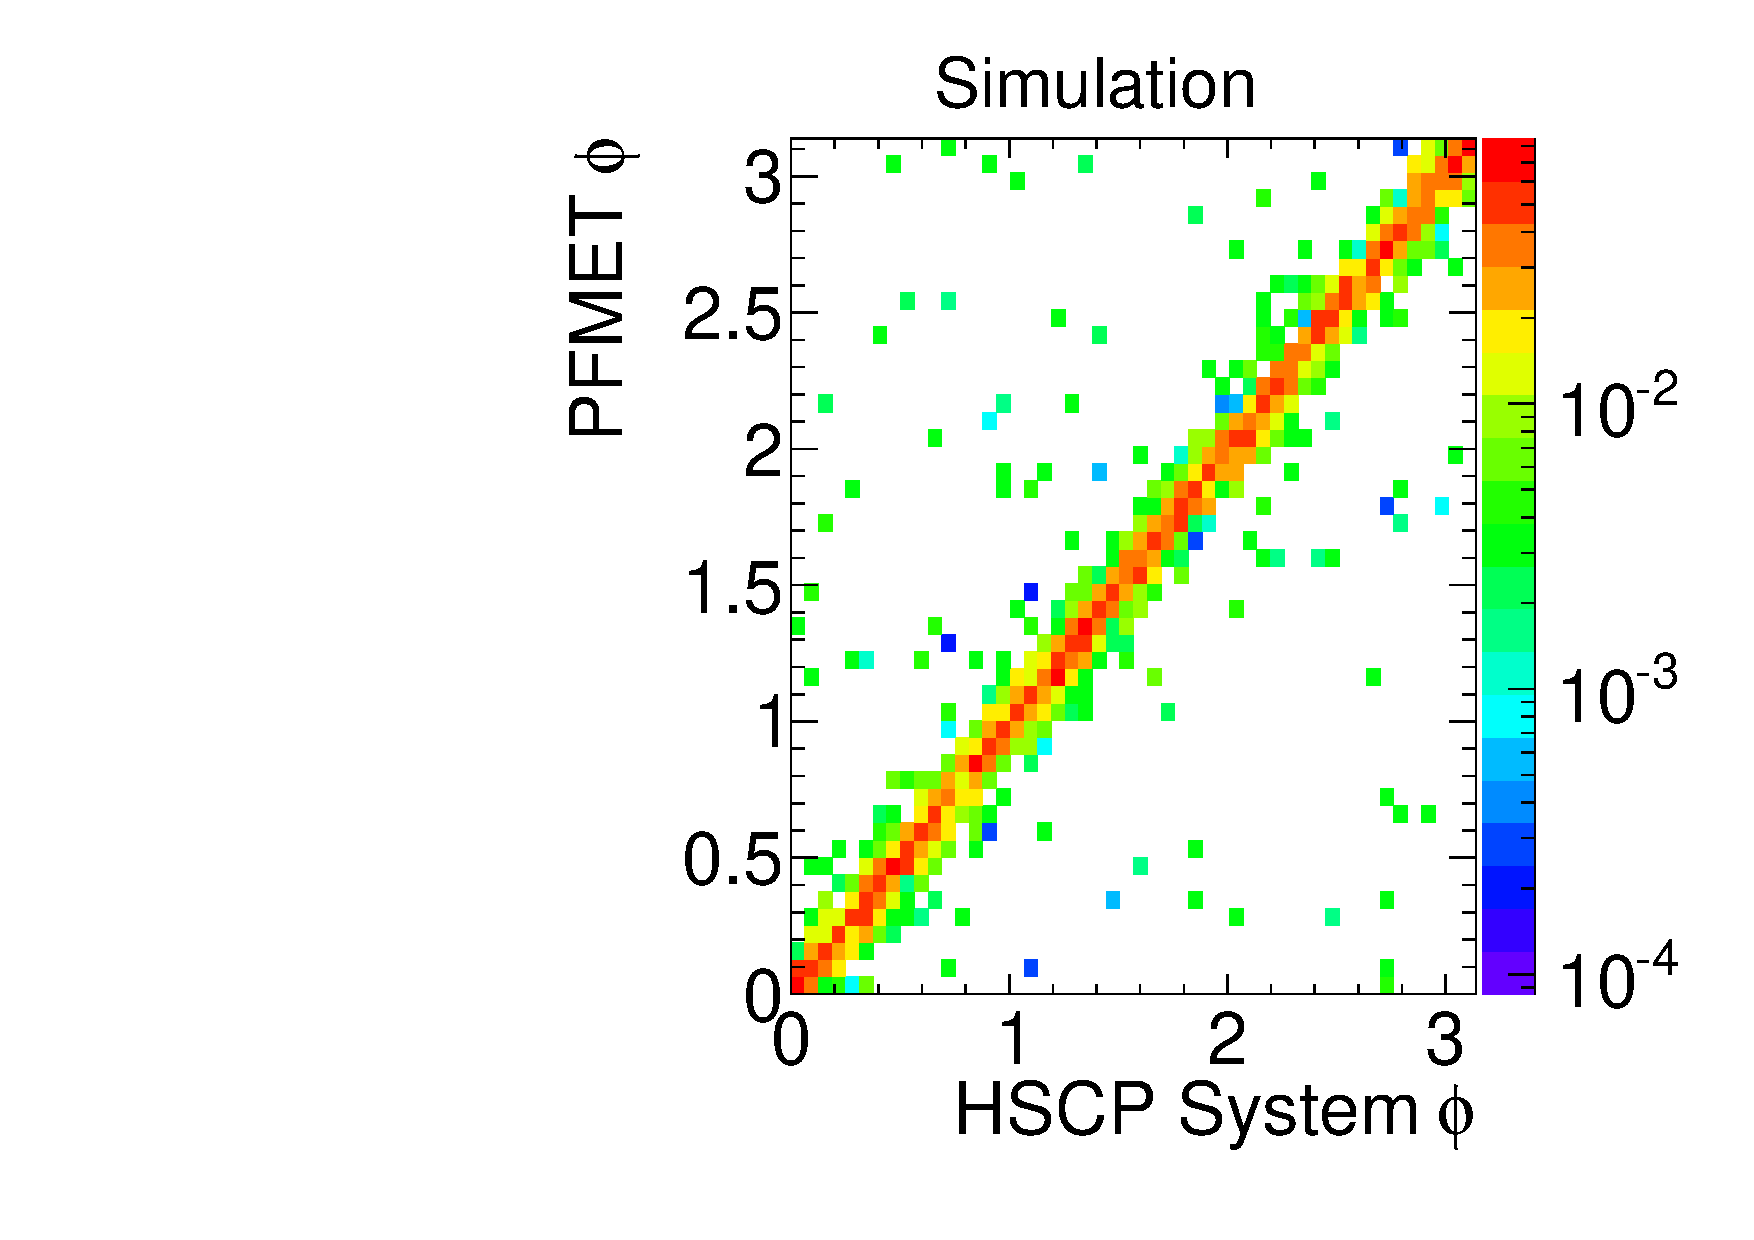
\includegraphics[clip=false, trim=0.0cm 0cm 0.0cm 0cm, width=0.49\textwidth]{figures/search/Gluino_8TeV_M1200_f100SystPhiMET}
      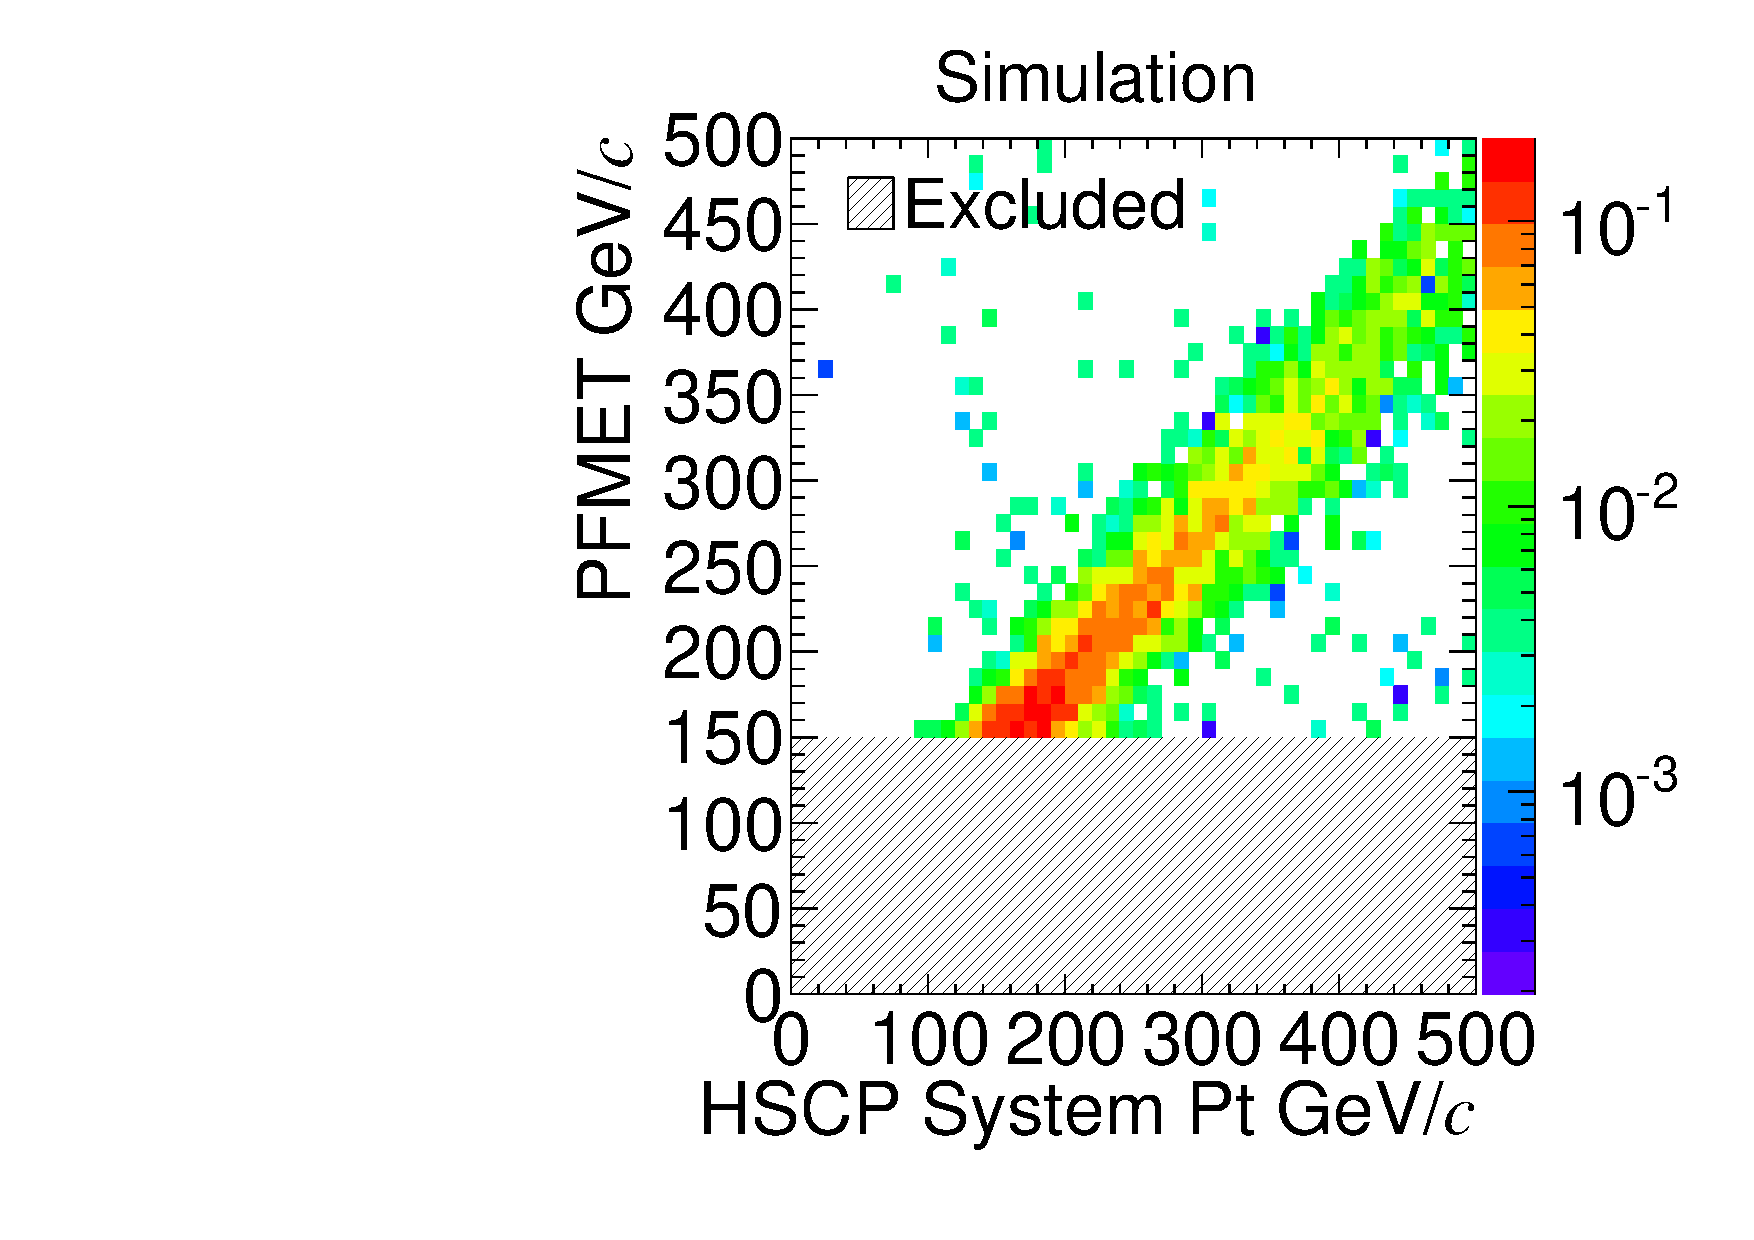
\includegraphics[clip=false, trim=0.0cm 0cm 0.0cm 0cm, width=0.49\textwidth]{figures/search/Gluino_8TeV_M1200_f100SystPtMET} \\
      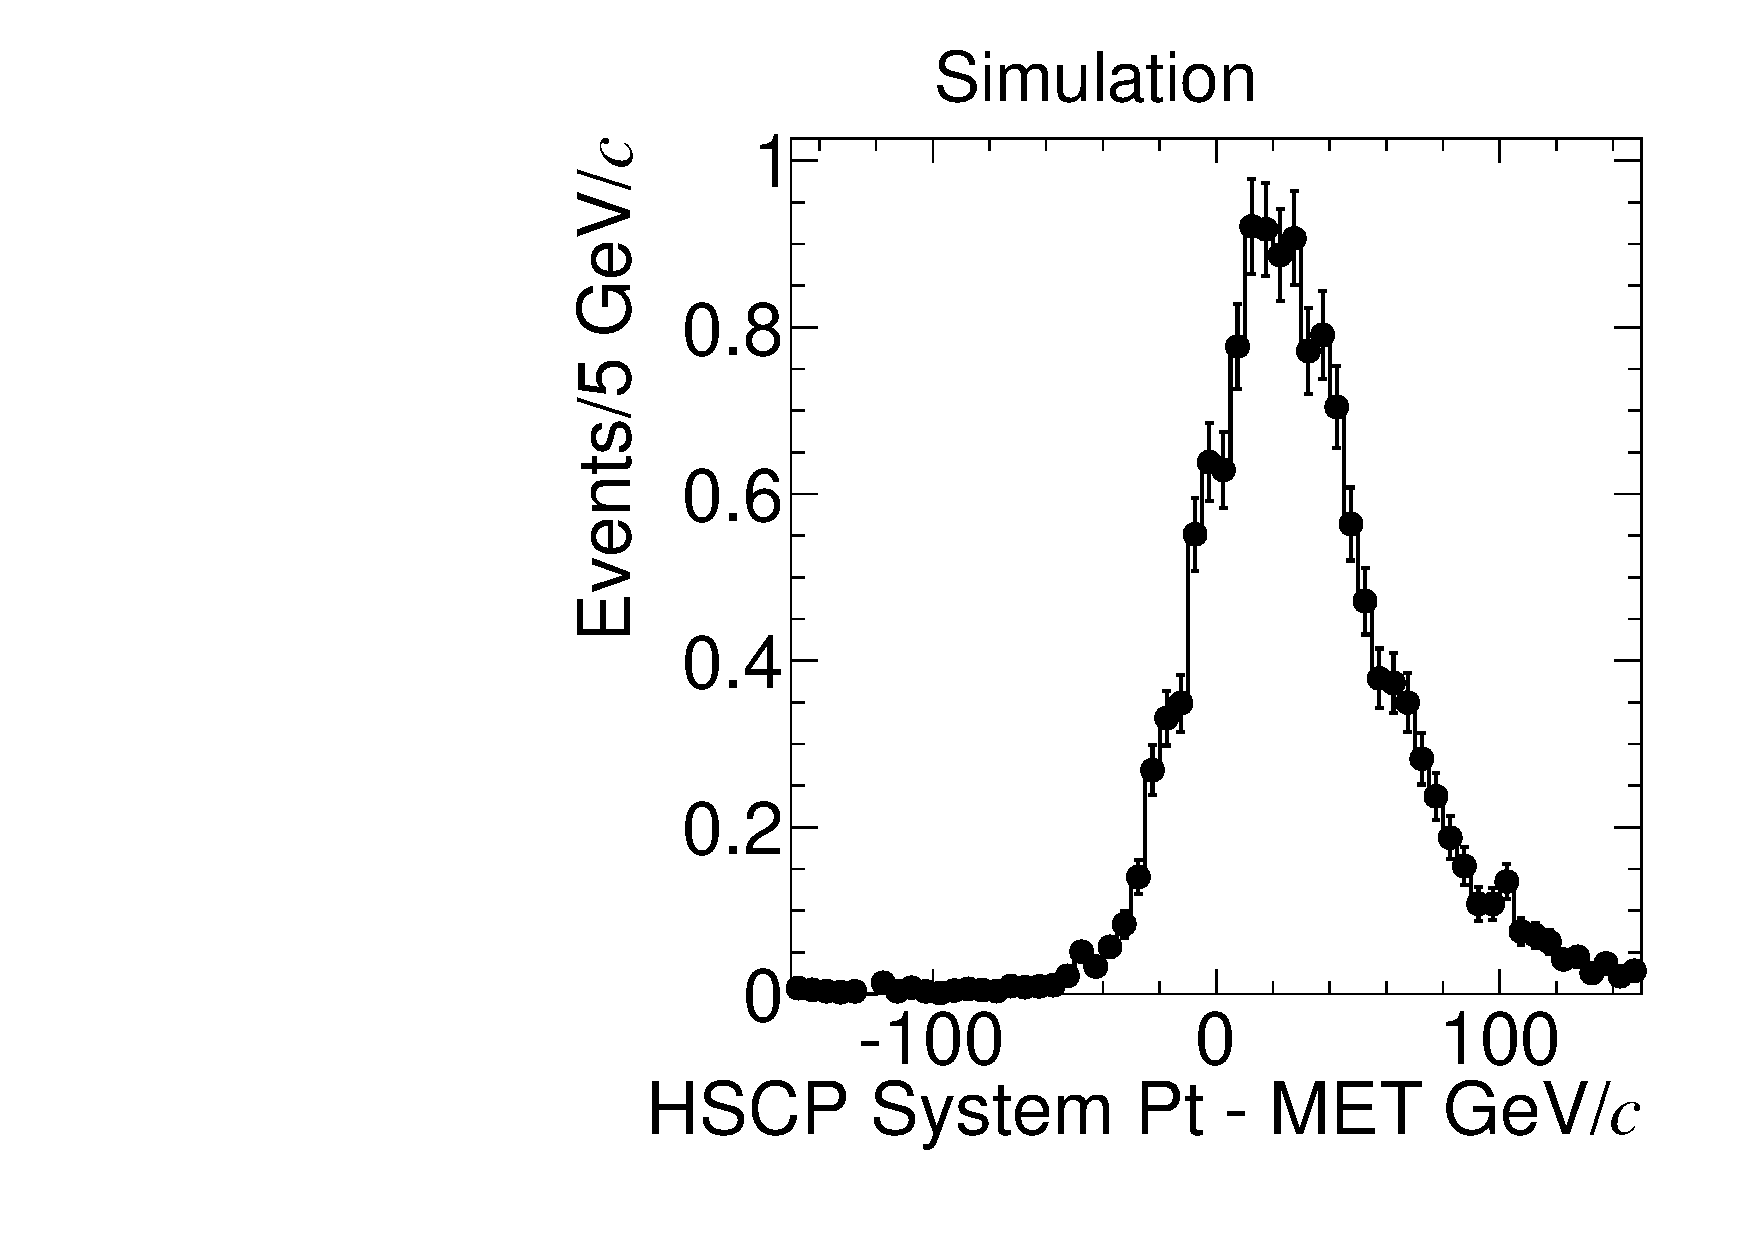
\includegraphics[clip=false, trim=0.0cm 0cm 0.0cm 0cm, width=0.49\textwidth]{figures/search/Gluino_8TeV_M1200_f100SystPtDiffMET}
      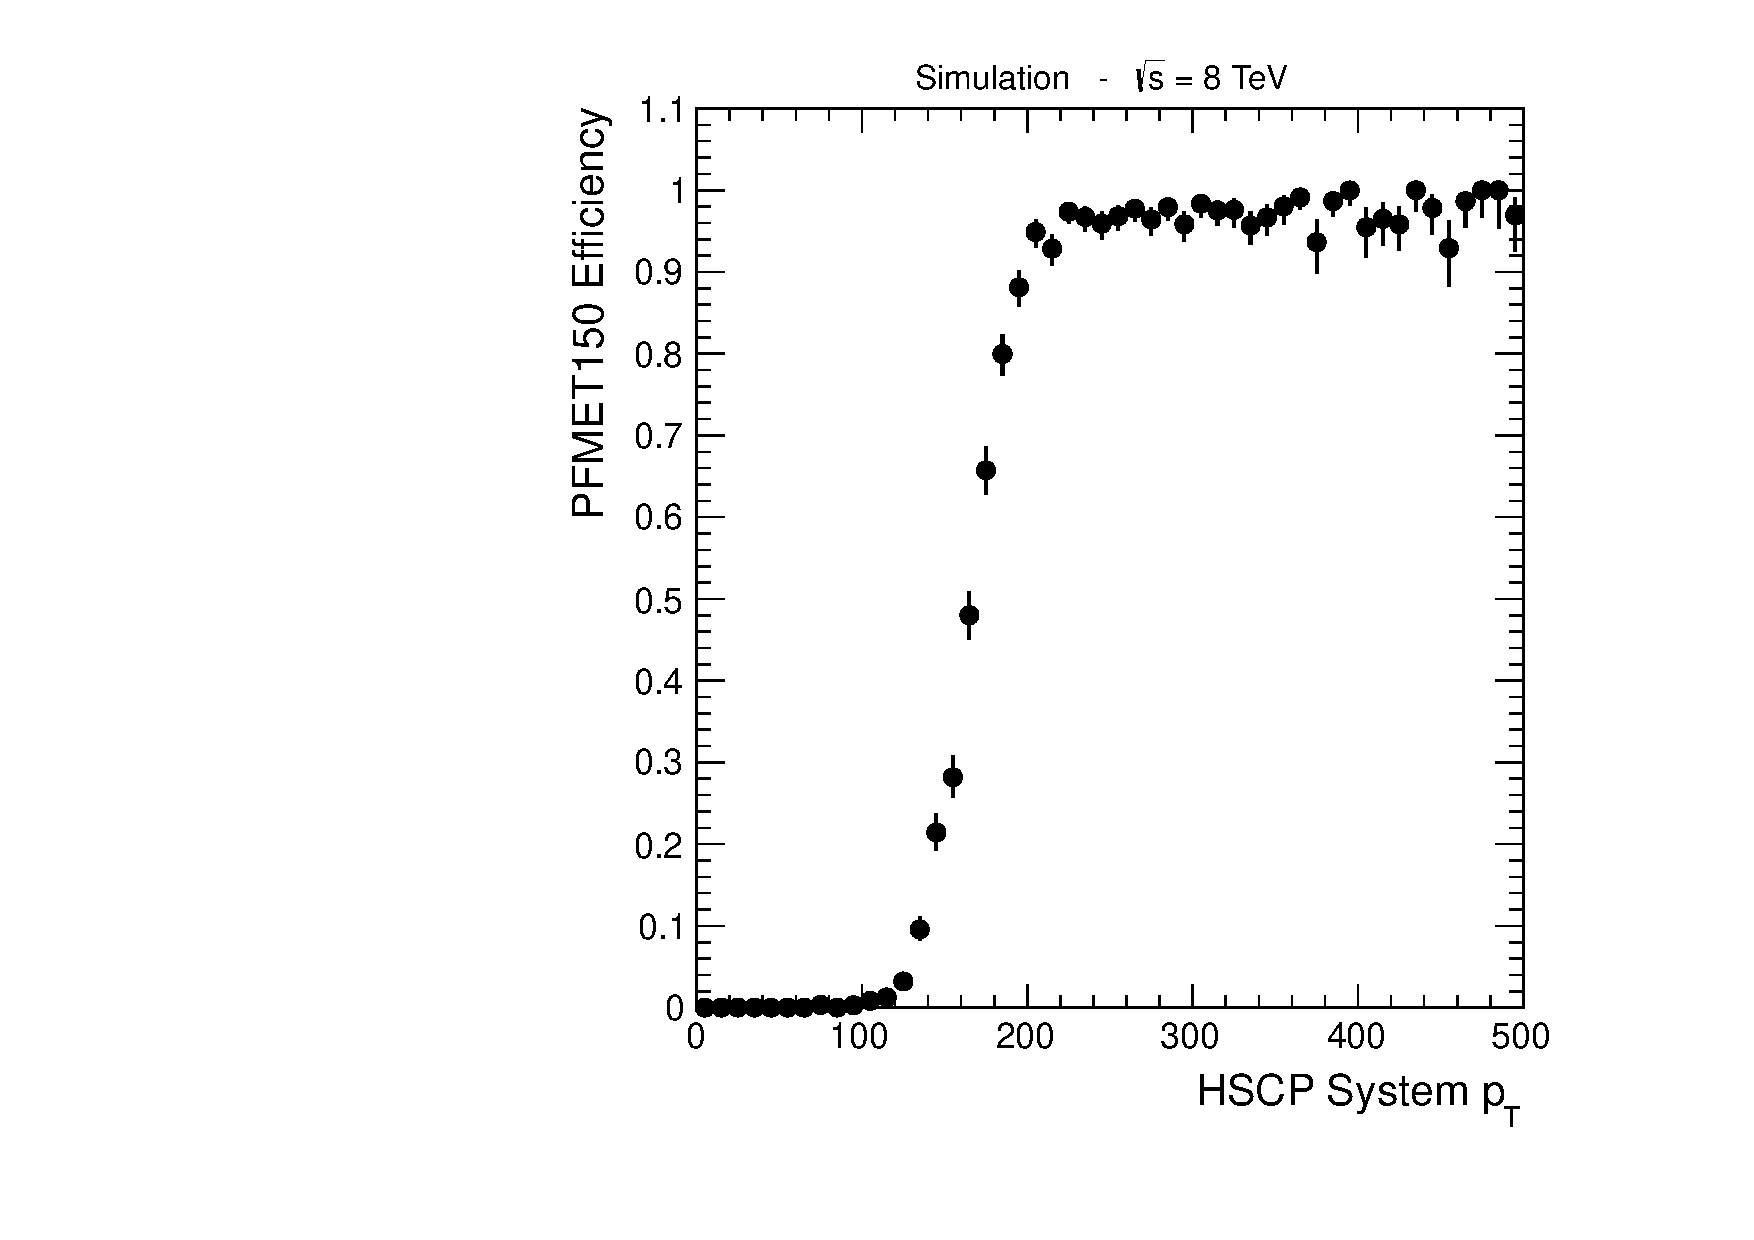
\includegraphics[clip=false, trim=0.0cm 0cm 0.0cm 0cm, width=0.49\textwidth]{figures/search/Gluino_8TeV_M1200_f100SystPtEff}
      \caption[Comparison of di-HSCP system $\phi$ and \pt\ with online PFMET for a 1200~GeV 
Gluino $f=1.0$ sample in events with at least 150~GeV of online PFMET.]
        {Comparison of di-HSCP system with online PFMET for a 1200~GeV Gluino $f=1.0$ sample in events with at least 150~GeV of online PFMET. 
         Top Left: Online PFMET $\phi$ versus di-HSCP system $\phi.$ Top Right: Online PFMET value versus di-HSCP system $p_T$. 
         Bottom Left: Difference between di-HSCP system $p_T$ and online PFMET value.
         Bottom Right: Probability to have online PFMET greater than 150~GeV versus di-HSCP system $p_T$. A horizontal dashed line is drawn at one.
        }
      \label{fig:SystPtTrigger}
  \end{center}
\end{figure}

\begin{figure}
  \begin{center}
      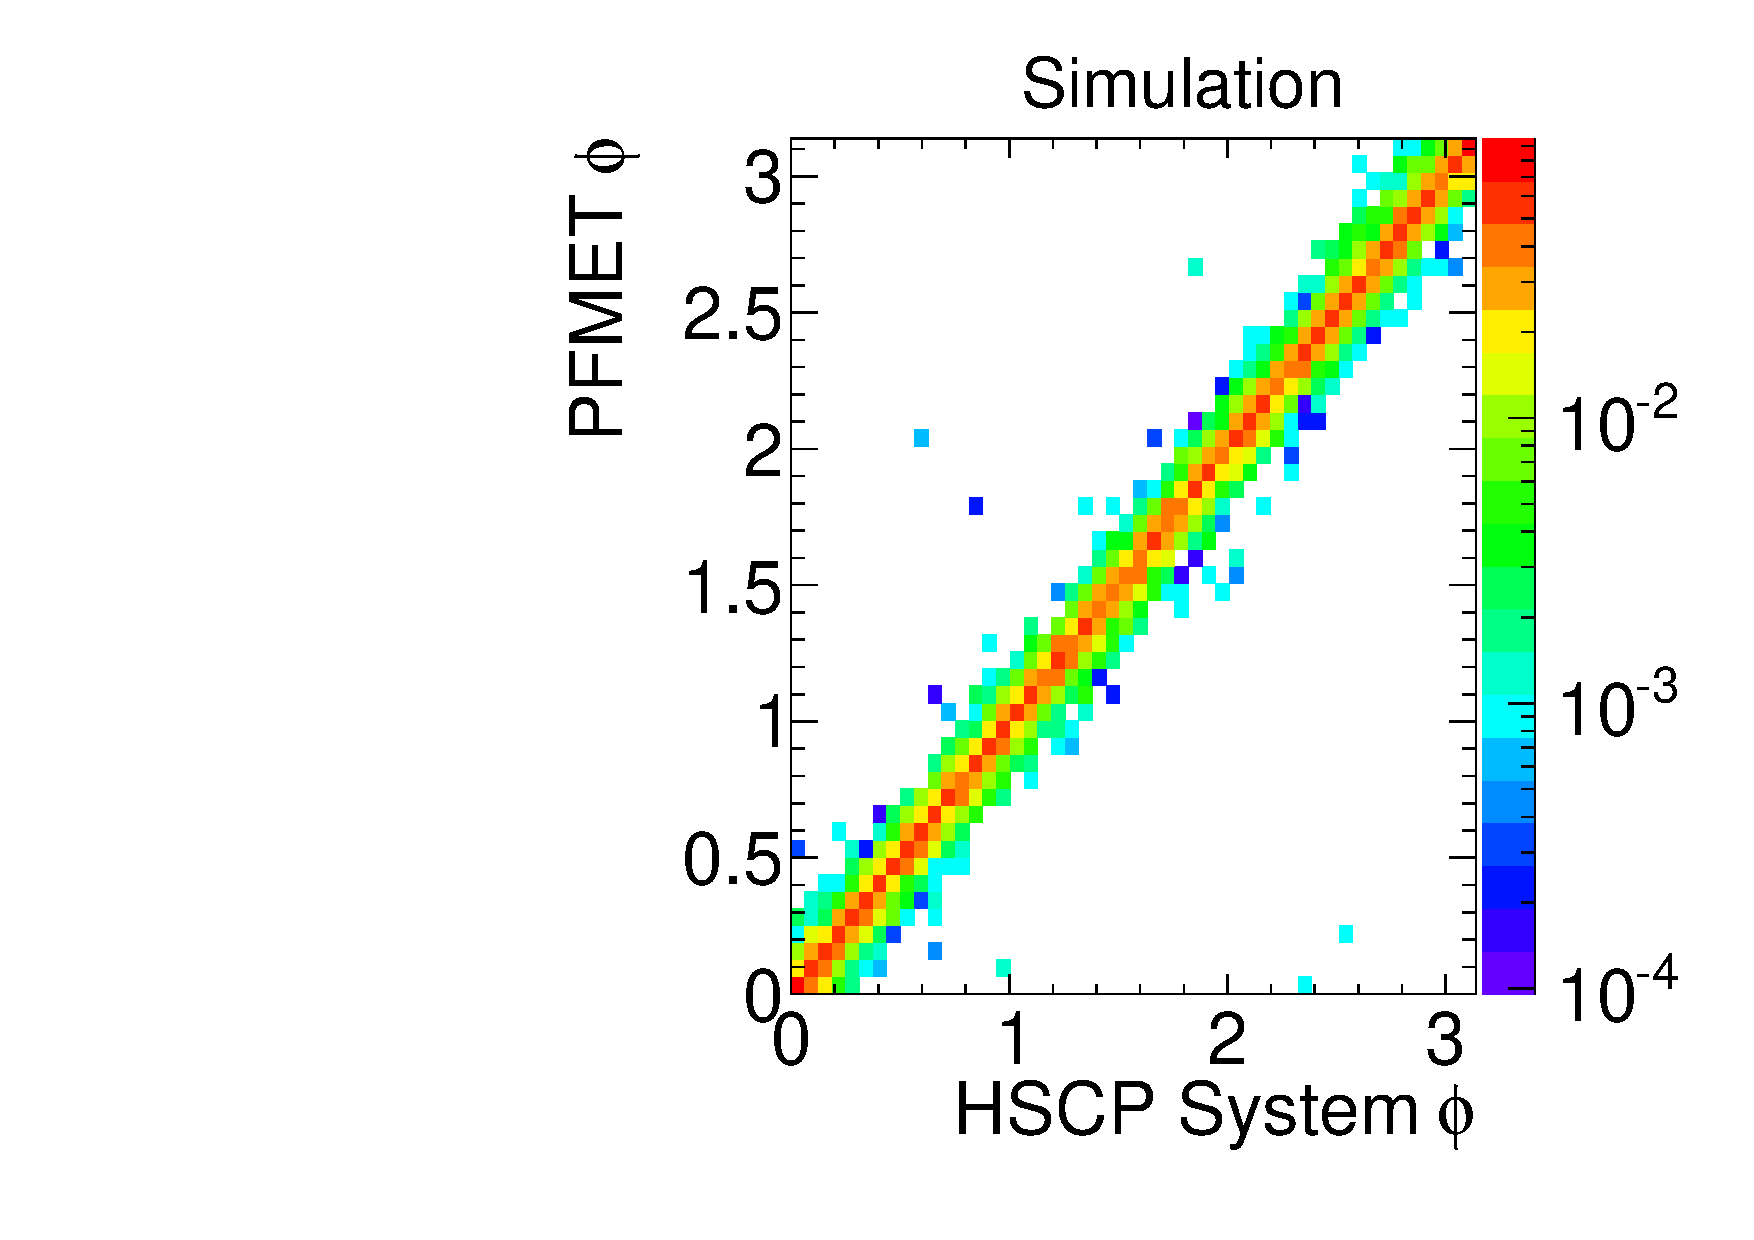
\includegraphics[clip=true, trim=0.0cm 0cm 3.0cm 0cm, width=0.49\textwidth]{figures/search/Gluino_8TeV_M1200N_f10SystPhiMET}
      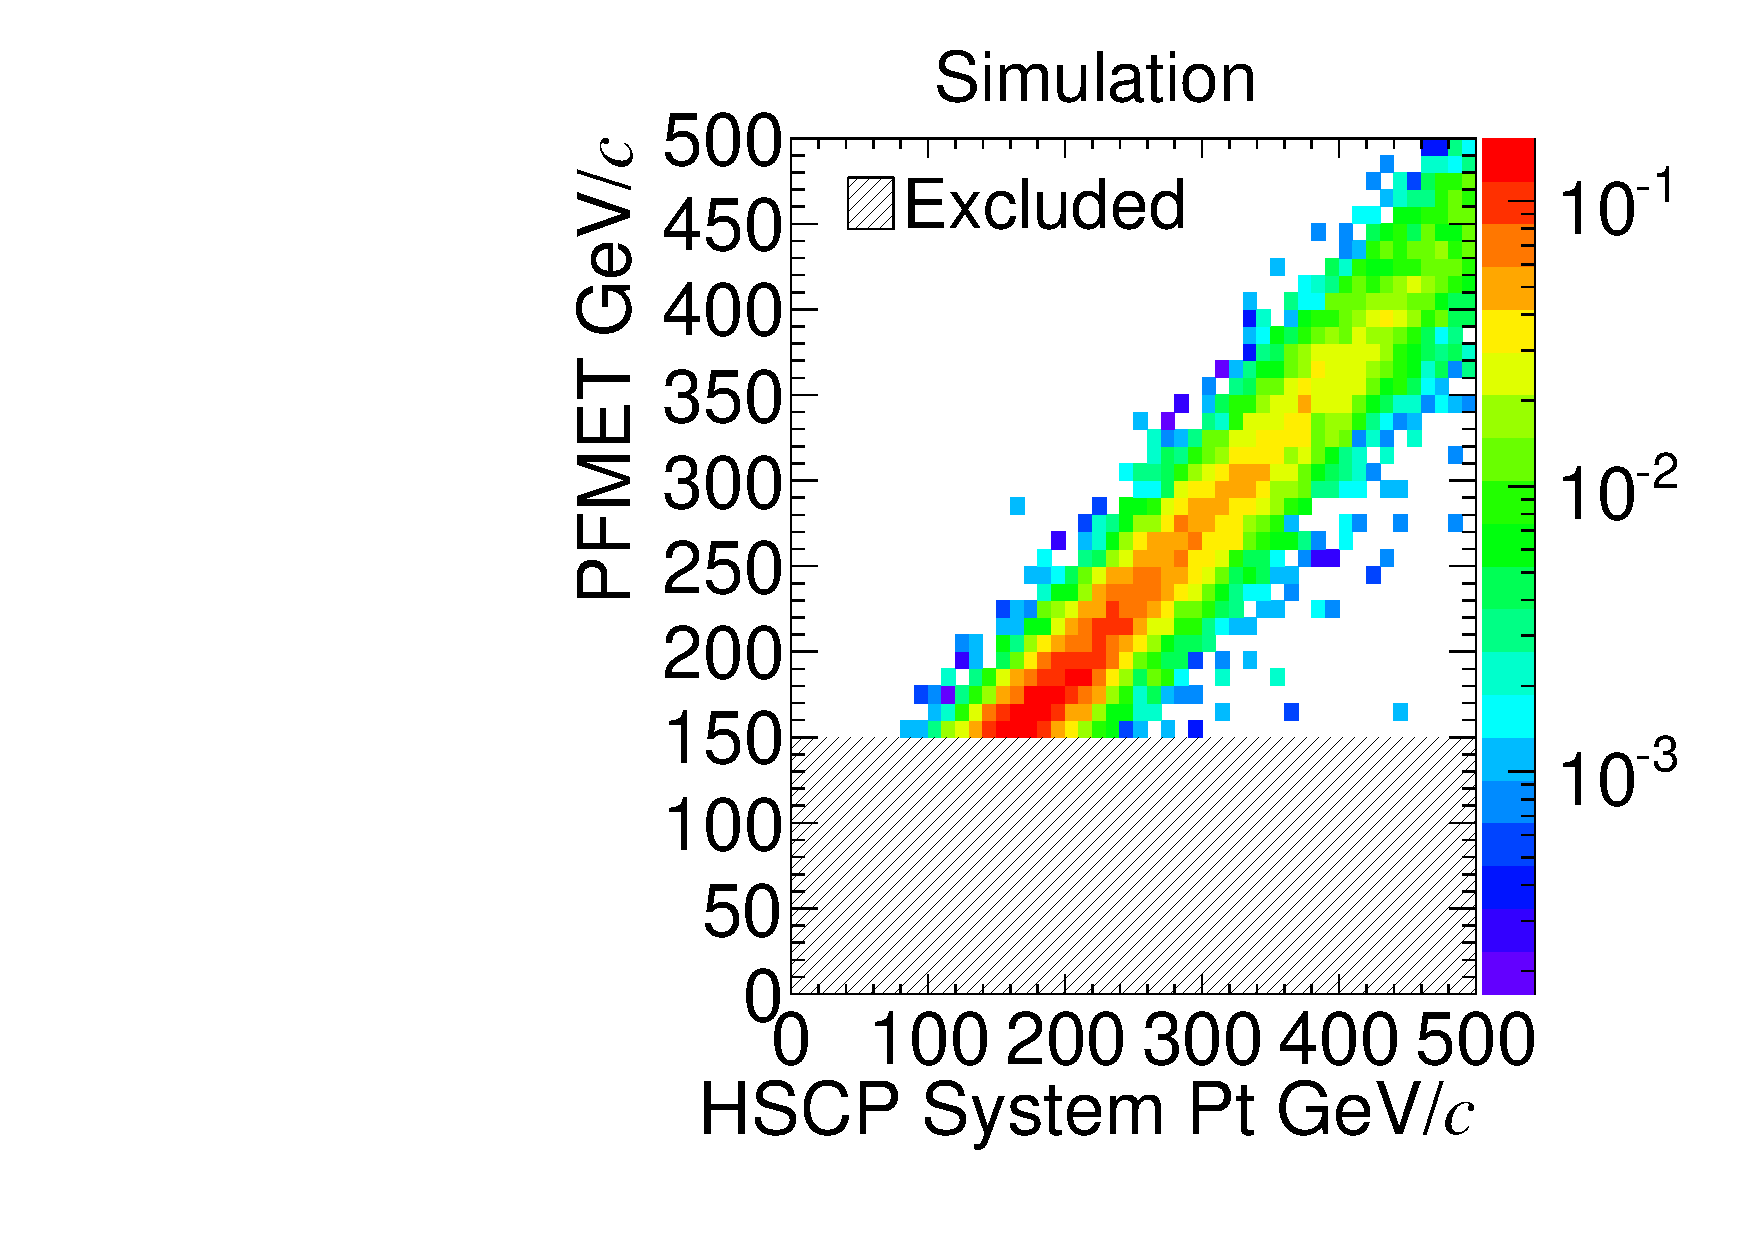
\includegraphics[clip=true, trim=0.0cm 0cm 3.0cm 0cm, width=0.49\textwidth]{figures/search/Gluino_8TeV_M1200N_f10SystPtMET} \\
      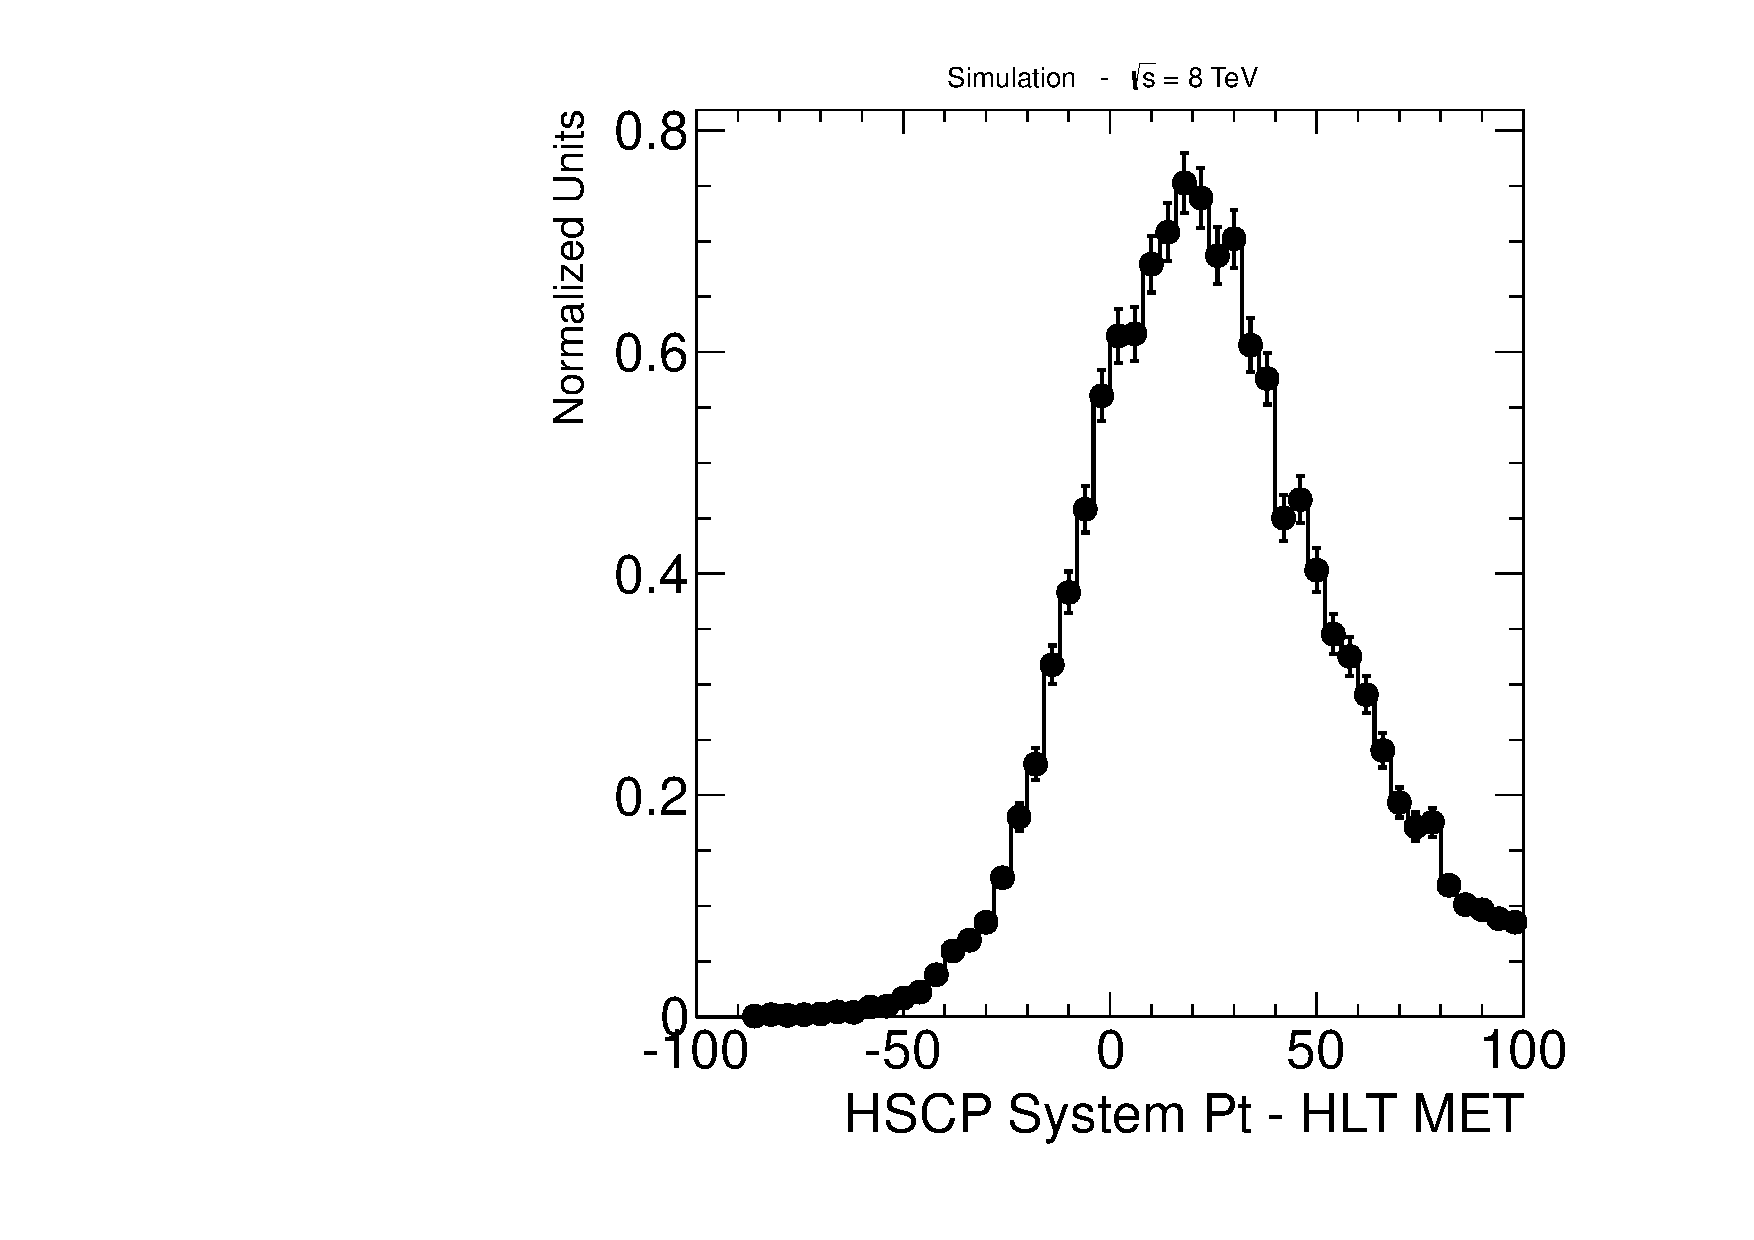
\includegraphics[clip=true, trim=0.0cm 0cm 3.0cm 0cm, width=0.49\textwidth]{figures/search/Gluino_8TeV_M1200N_f10SystPtDiffMET}
      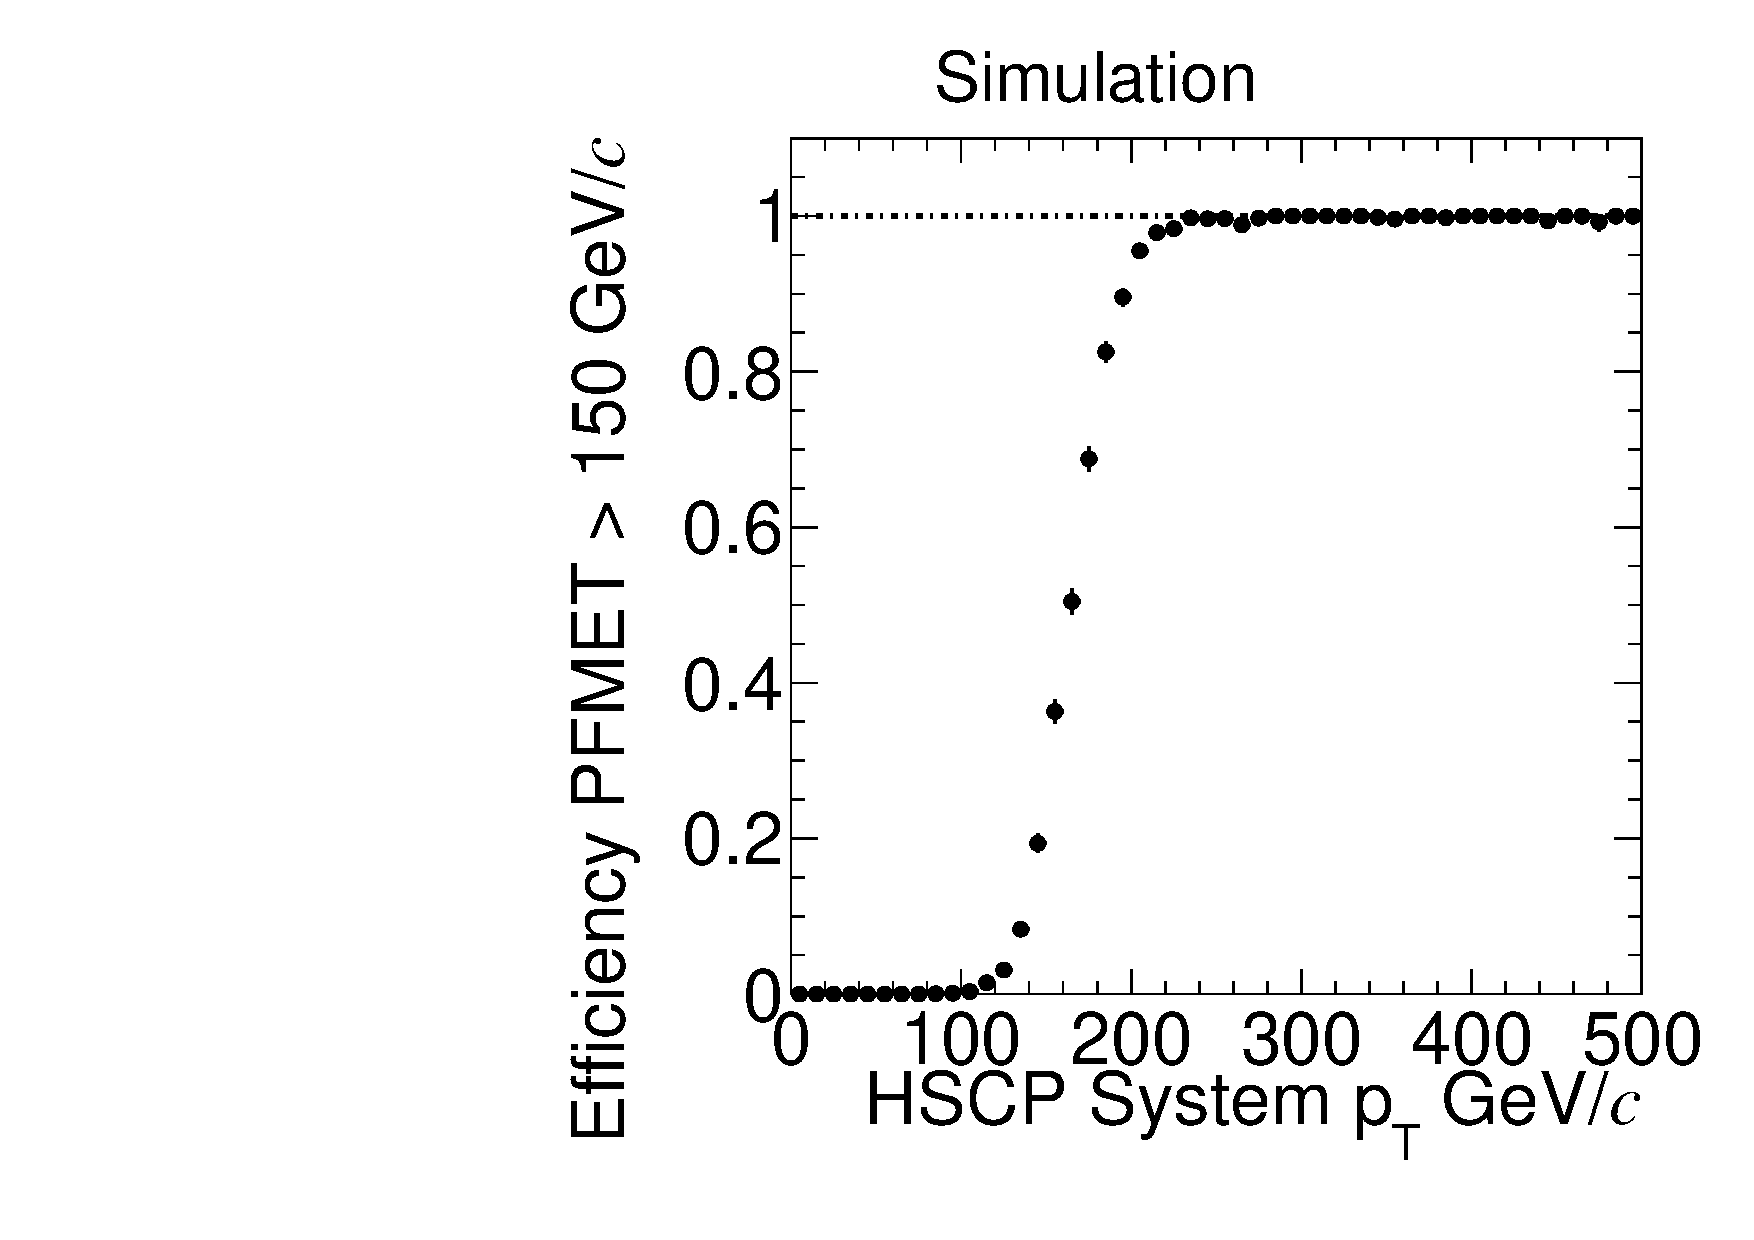
\includegraphics[clip=true, trim=0.0cm 0cm 3.0cm 0cm, width=0.49\textwidth]{figures/search/Gluino_8TeV_M1200N_f10SystPtEff}
      \caption[Comparison of di-HSCP system $\phi$ and \pt\ with online PFMET for a 1200~GeV
Gluino $f=0.1$ charge suppressed sample in events with at least 150~GeV of online PFMET]
      {Same as Fig.~\ref{fig:SystPtTrigger} but the sample used is 1200~GeV $f=0.1$ charge suppressed gluino.
%Comparison of di-HSCP system with online PFMET for a charge suppressed 1200 GeV Gluino $f=0.1$ sample in events with at least 150 GeV of online PFMET.
%         Top Left: Online PFMET $\phi$ versus di-HSCP system $\phi.$ Top Right: Online PFMET value versus di-HSCP system $p_T$.
%         Bottom Left: Difference between di-HSCP system $p_T$ and online PFMET value.
%         Bottom Right: Probability to have online PFMET greater than 150 versus di-HSCP system $p_T$.
        }
      \label{fig:SystPtTriggerN}
  \end{center}
\end{figure}

One trigger issue unique to slow-moving particles is the timing acceptance of the L1 trigger. If an HSCP arrives in the muon system too late, it can trigger the
readout of the wrong bunch crossing. As most of the CMS subdetectors, though not the muon system, are designed to not readout data coming from adjacent bunch crossings,
the data from the correct bunch crossing would be lost. To help deal with this, members of the CMS L1 trigger team developed a special configuration of the
RPC L1 trigger to partially recover HSCP that arrive in the muon system in the bunch crossing window following the crossing that produced them.
This configuration is discussed in Sec.~\ref{sec:computing}.

%The configuration creates a duplicate copy of all RPC hits and sends them to the muon trigger in the bunch crossing immediately preceding the arrival of the hits. 
%This allows for HSCP that
%arrive in the RPCs 0.5 -- 1.5 bunch crossings later than a collision muon would to still trigger the readout of the correct event. For particles that arrive in the RPC
%in the correct bunch crossing, a coincidence with the LHC beam crossing through CMS is required to prevent the readout of the previous event. This configuration
%was possible for 2012 running as the proton bunches were separated by 50ns despite having 25ns wide bunch crossing window windows.
%The configuration is described in more detail in Sec.~\ref{sec:computing}.

The first algorithm used requires both a high-momentum track to be found in the muon system and large PFMET.
For the first 0.7~fb$^{-1}$ of 2012 running the threshold on PFMET was at 65~GeV. The signal samples are weighted
to account for the amount of data taken at each threshold.
The algorithm starts at the L1 step where a track must be found in the muon system by the detector electronics with a momentum greater than 16~GeV and $\eta$ less than 2.1 
in order to trigger the readout of the event to the computing farm.
There, the L1 track is used during the L2 step to seed the reconstruction of the track using only data readout from the muon system.
The track is required to have $p_T > 70$~GeV, $|\eta| < 2.1$, and hits in at least two muon stations.
In the L3 step, the particle flow algorithm is run and the calculated PFMET must be greater than 55 GeV.
For the first 0.7~fb$^{-1}$ of 2012 running the threshold on PFMET was at 65~GeV. The signal samples are weighted
to account for the amount of data taken at each threshold.

The lack of a requirement that the track be found in the silicon tracker allows the trigger to be sensitive to $R$-hadrons produced neutral and only later becoming charged.
The main objective of the PFMET requirement is to reduce the rate of events collected by the trigger
down to a few Hertz. The momentum measurement by the muon system suffers from long tails and the rate would be too large even with a very high momentum threshold.
Events collected with this trigger are only used in the \muononly\ analysis.

The second algorithm requires a high momentum track matched in both the silicon tracker and muon system be found.
During the L1 and L2 steps, the algorithm follows the same steps as the above trigger with the only exception being that $p_T$ threshold on the L2 track
is reduced to 16~GeV. During the L3 step, the L2 track is used to seed the reconstruction of tracks that span from the silicon tracker to the muon system.
A track must be found with momentum greater than 40~GeV and $\eta <$ 2.1. The very good resolution of the silicon tracker allows for an acceptable trigger rate
without any further requirements. Events collected with this trigger are only used in all analyses.

The only requirement for the third algorithm is PFMET $ > 150$~GeV.
The second and third algorithms are used in all the analyses.

The decision to use the pure PFMET trigger even when a muon signature is required offline is prompted by the late arrival of the HSCPs in the muon system.
Even with the RPC configuration described above, very slow moving HSCP can trigger the readout of the wrong event but still be reconstructed offline
if the event has been triggered by the pure PFMET trigger. This can be seen in Figure~\ref{fig:TriggerEffVsBetaGl} which shows the trigger efficiency versus $\beta$
with and without the pure PFMET trigger.
It can be seen that using the pure PFMET trigger allows the search to probe lower $\beta$ particles. 

%Additional triggers were developed to collect - Maybe add dE/dx triggers?

%As color charged $R$-hadron can be neutral
%while traversing CMS or arrive so late to the muon system that they are not able to be reconstructed offline an effective detector acceptance is defined 
%that at least one HSCP be reconstructed offline. Thus Figure~\ref{fig:TriggerEffVsBetaGl} shows the efficiency requiring an HSCP be reconstructed as a track
%as in the \muononly\ analysis, and as a global track, as in the the \tktof\ analysis.

\begin{figure}
\centering
%  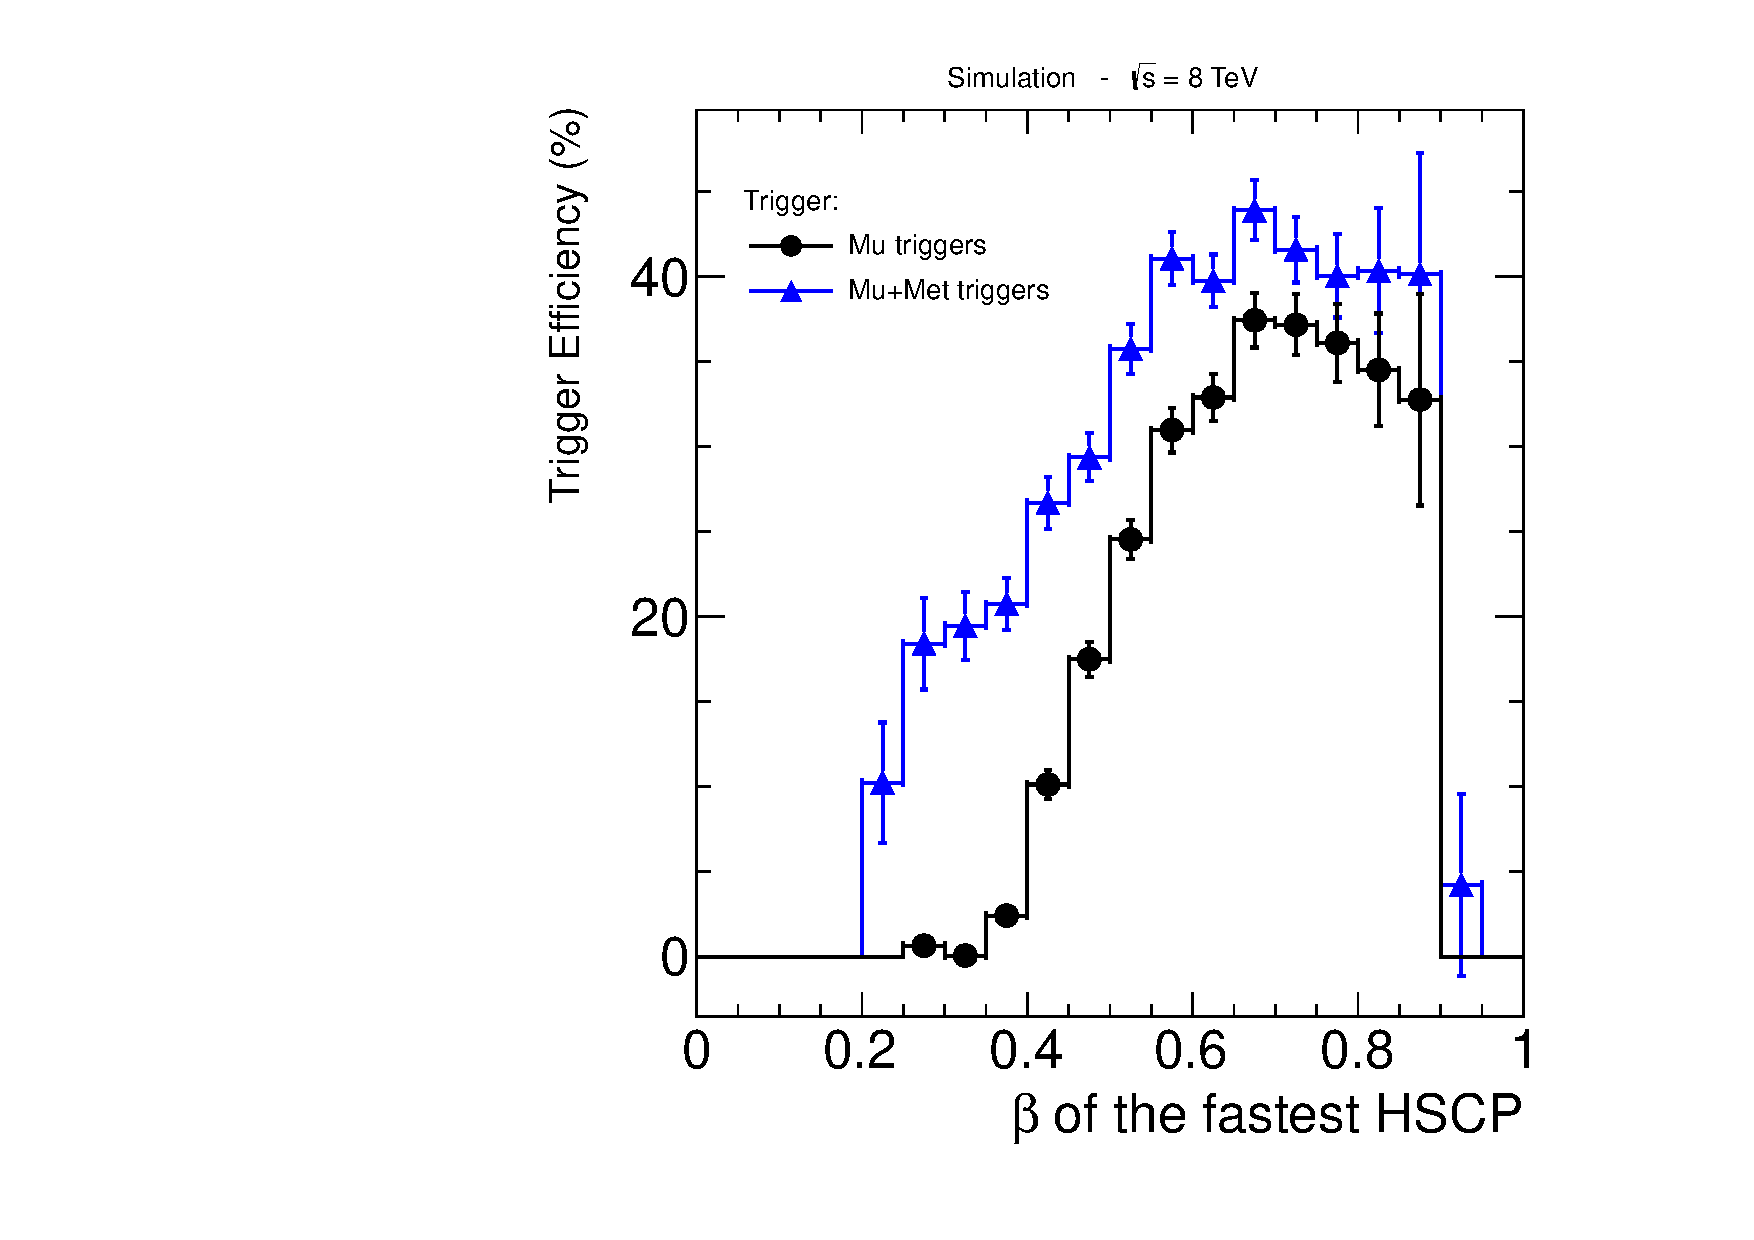
\includegraphics[clip=true, trim=0.0cm 0cm 3.0cm 0cm, width=0.49\textwidth]{figures/search/Gluino_8TeV_M1200_f100MatchedSA}
  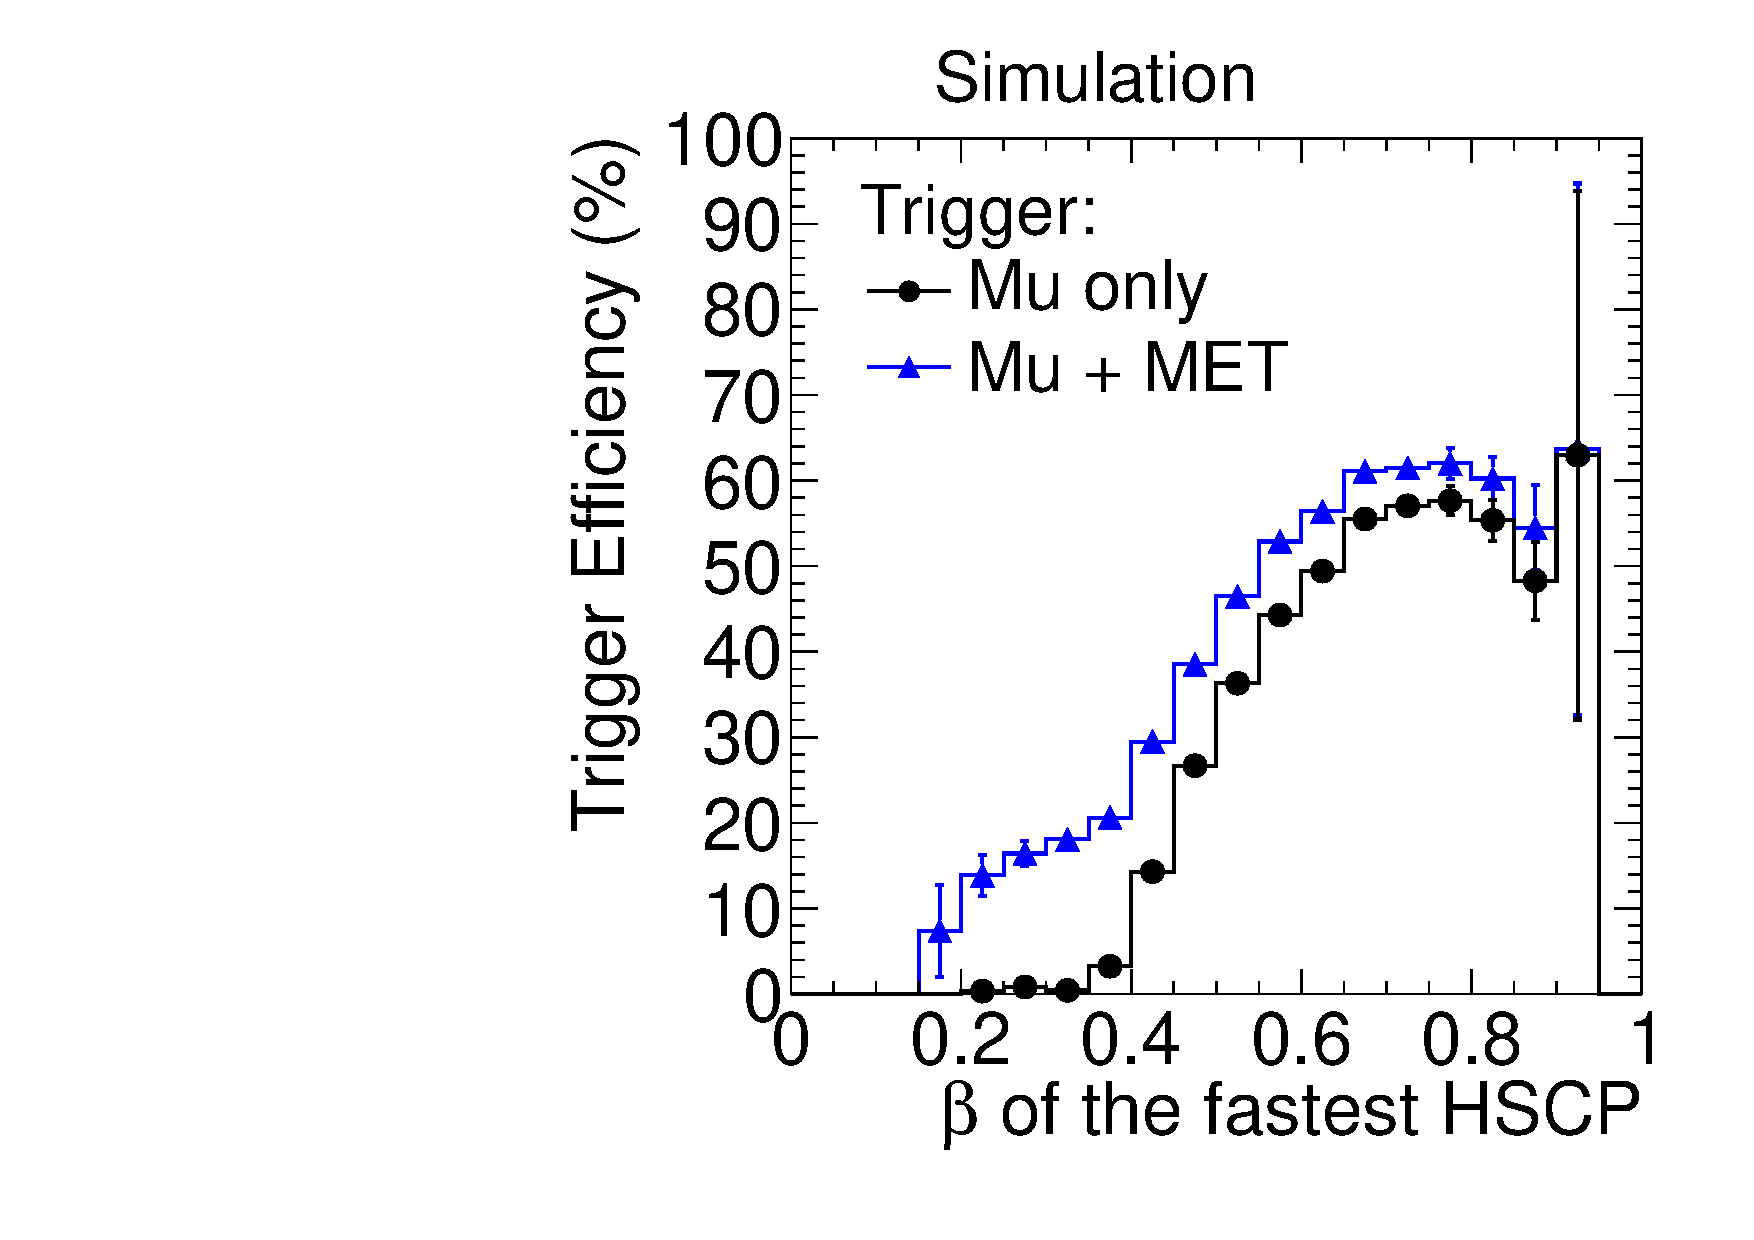
\includegraphics[clip=true, trim=0.0cm 0cm 3.0cm 0cm, width=0.49\textwidth]{figures/search/Gluino_8TeV_M1200_f10MatchedSA}
  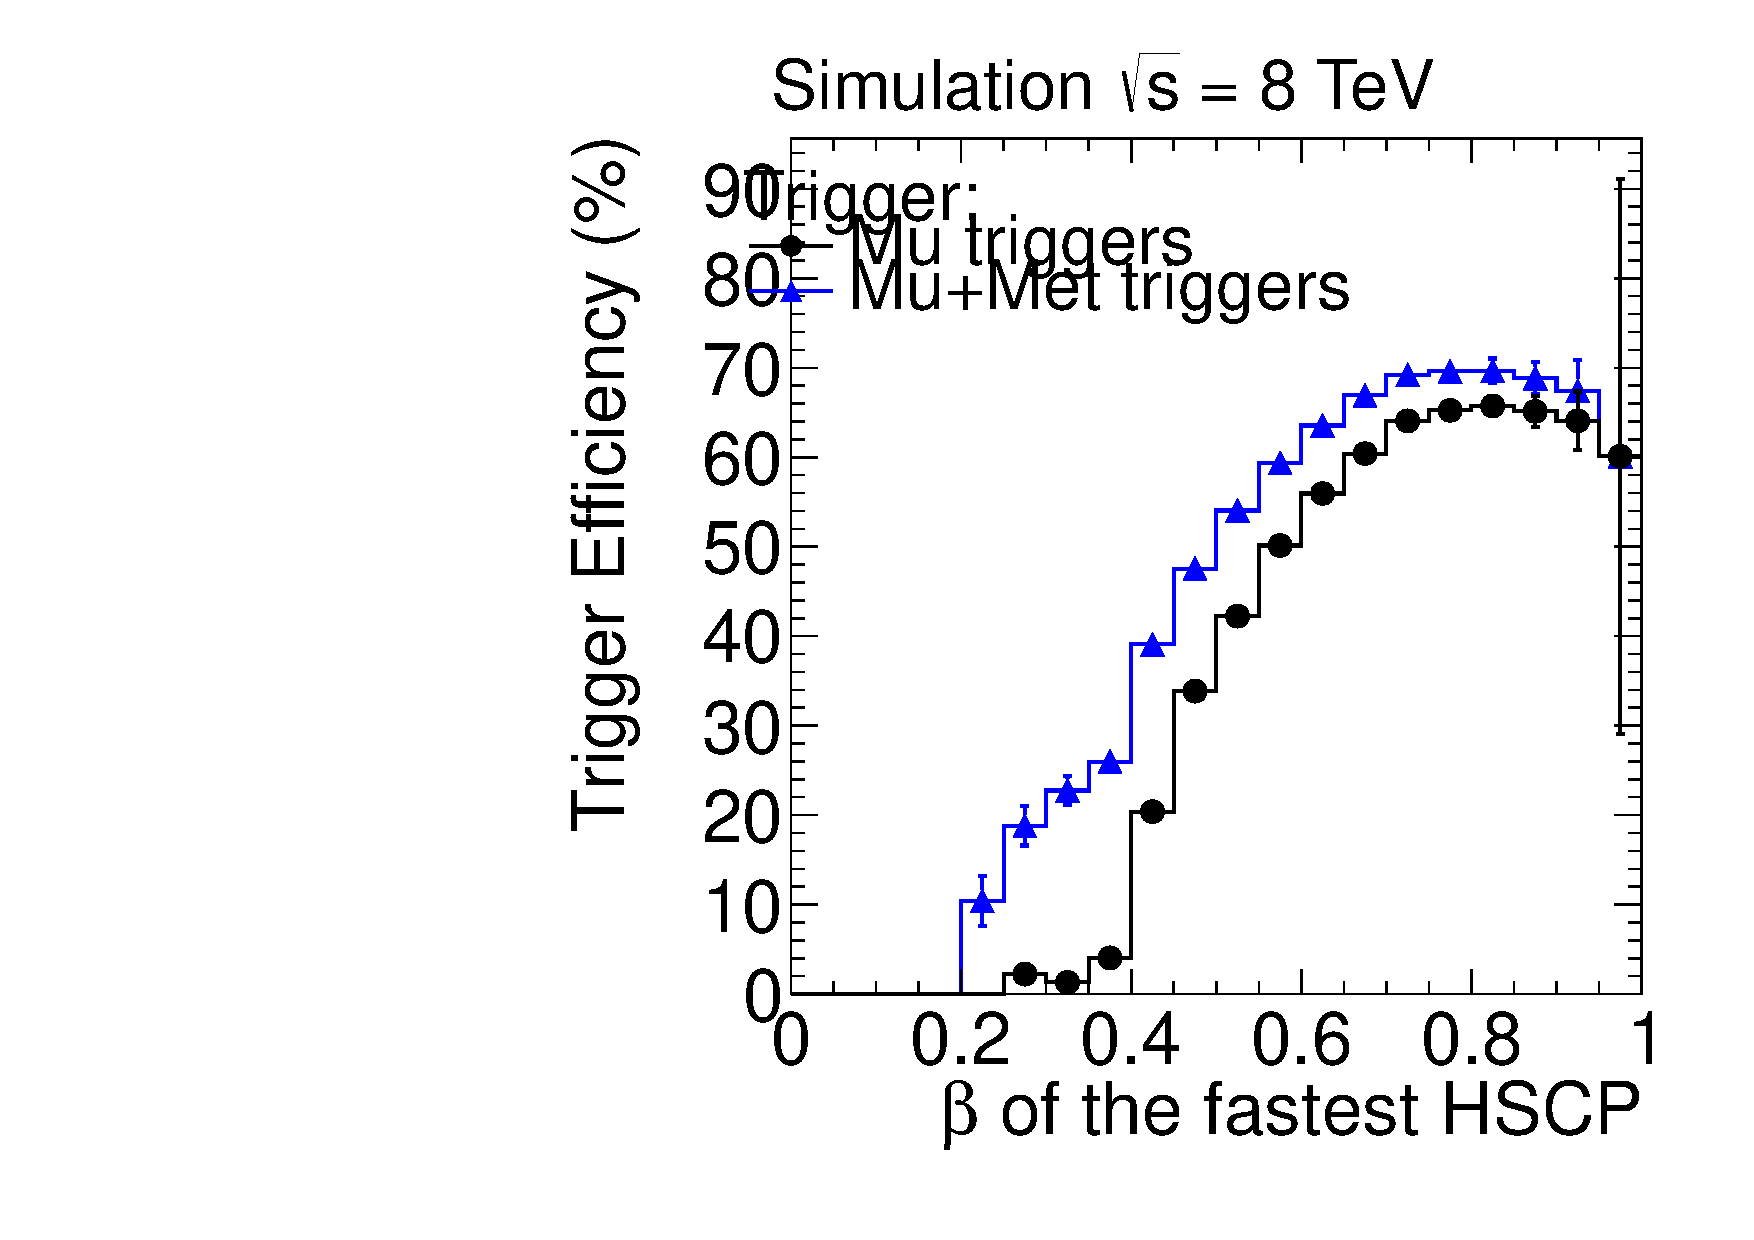
\includegraphics[clip=true, trim=0.0cm 0cm 3.0cm 0cm, width=0.49\textwidth]{figures/search/Stop_8TeV_M800MatchedSA}
%  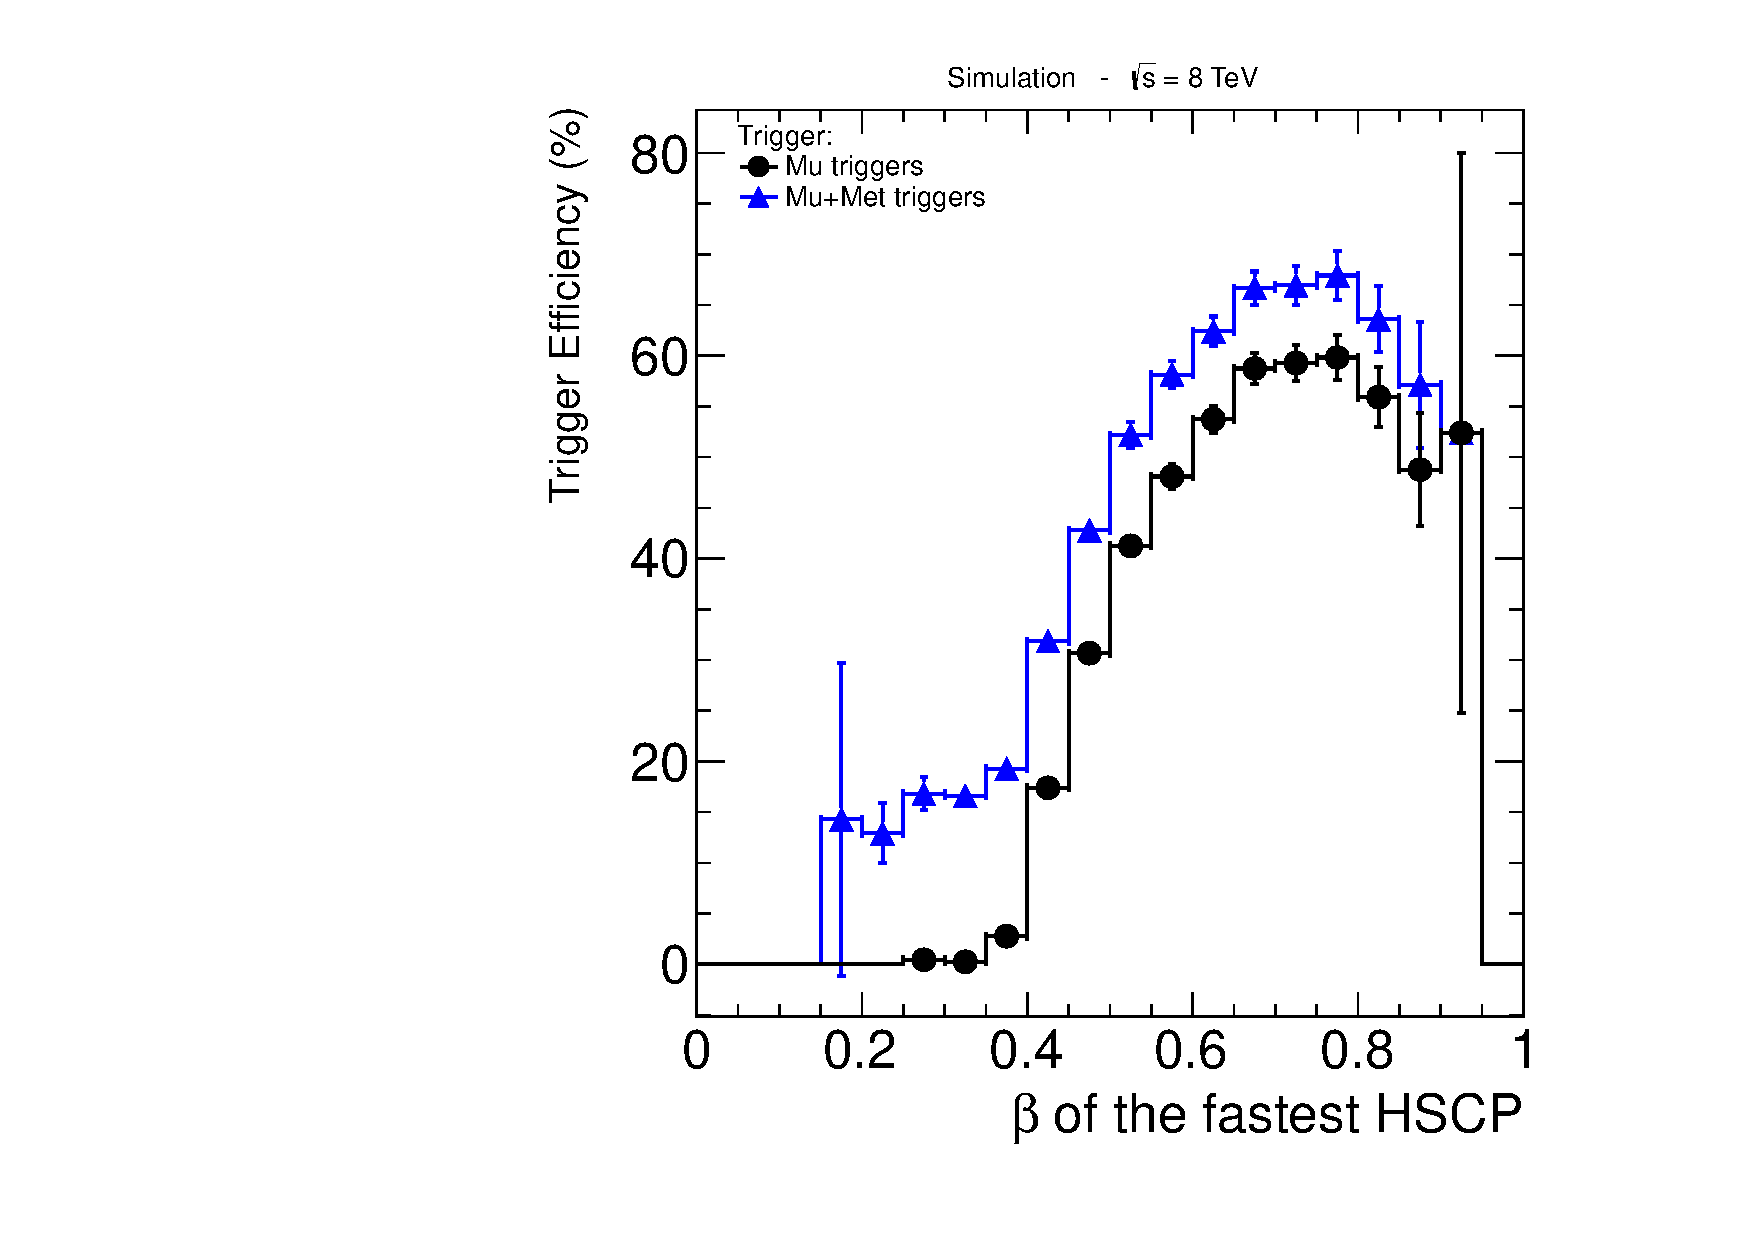
\includegraphics[clip=true, trim=0.0cm 0cm 3.0cm 0cm, width=0.32\textwidth]{figures/search/Gluino_8TeV_M1200_f10MatchedGl}
%  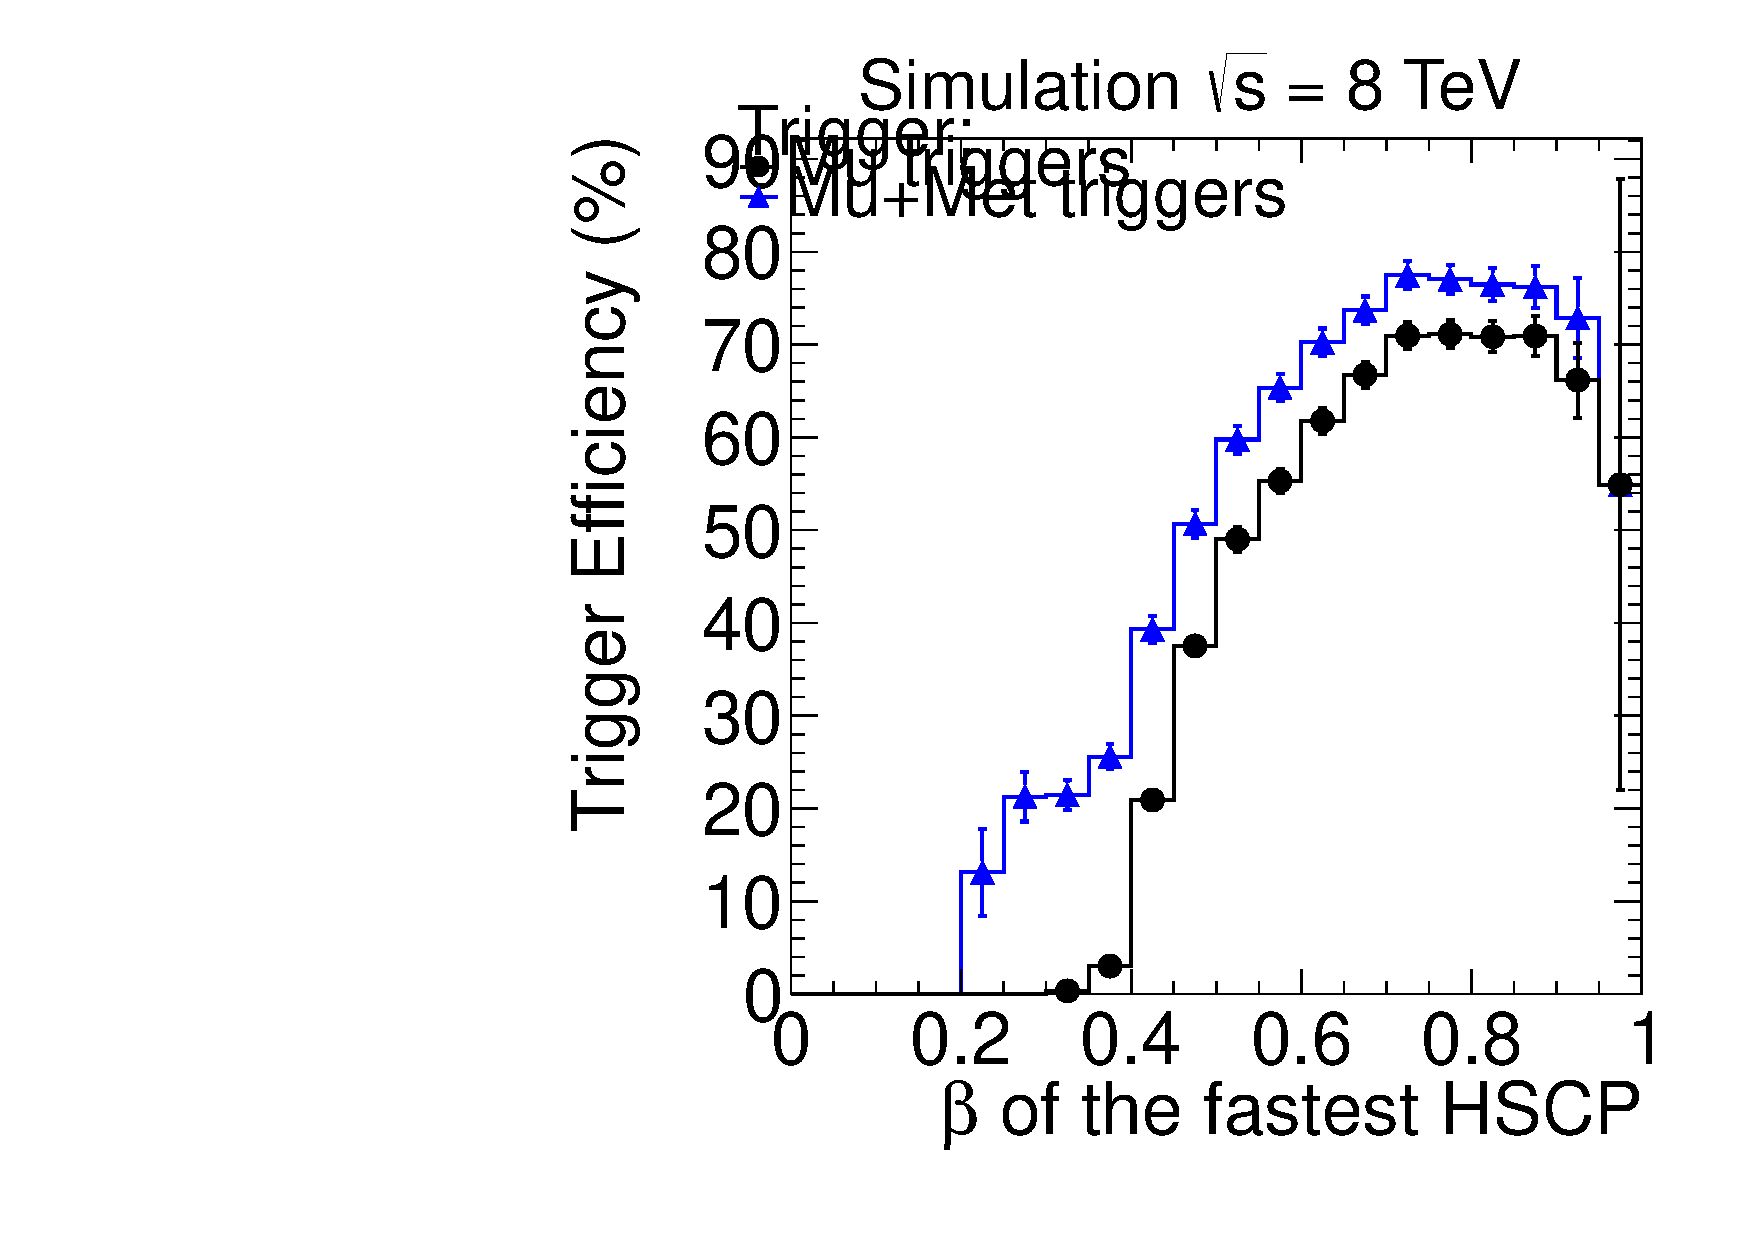
\includegraphics[clip=true, trim=0.0cm 0cm 3.0cm 0cm, width=0.32\textwidth]{figures/search/Stop_8TeV_M800MatchedGl}
%  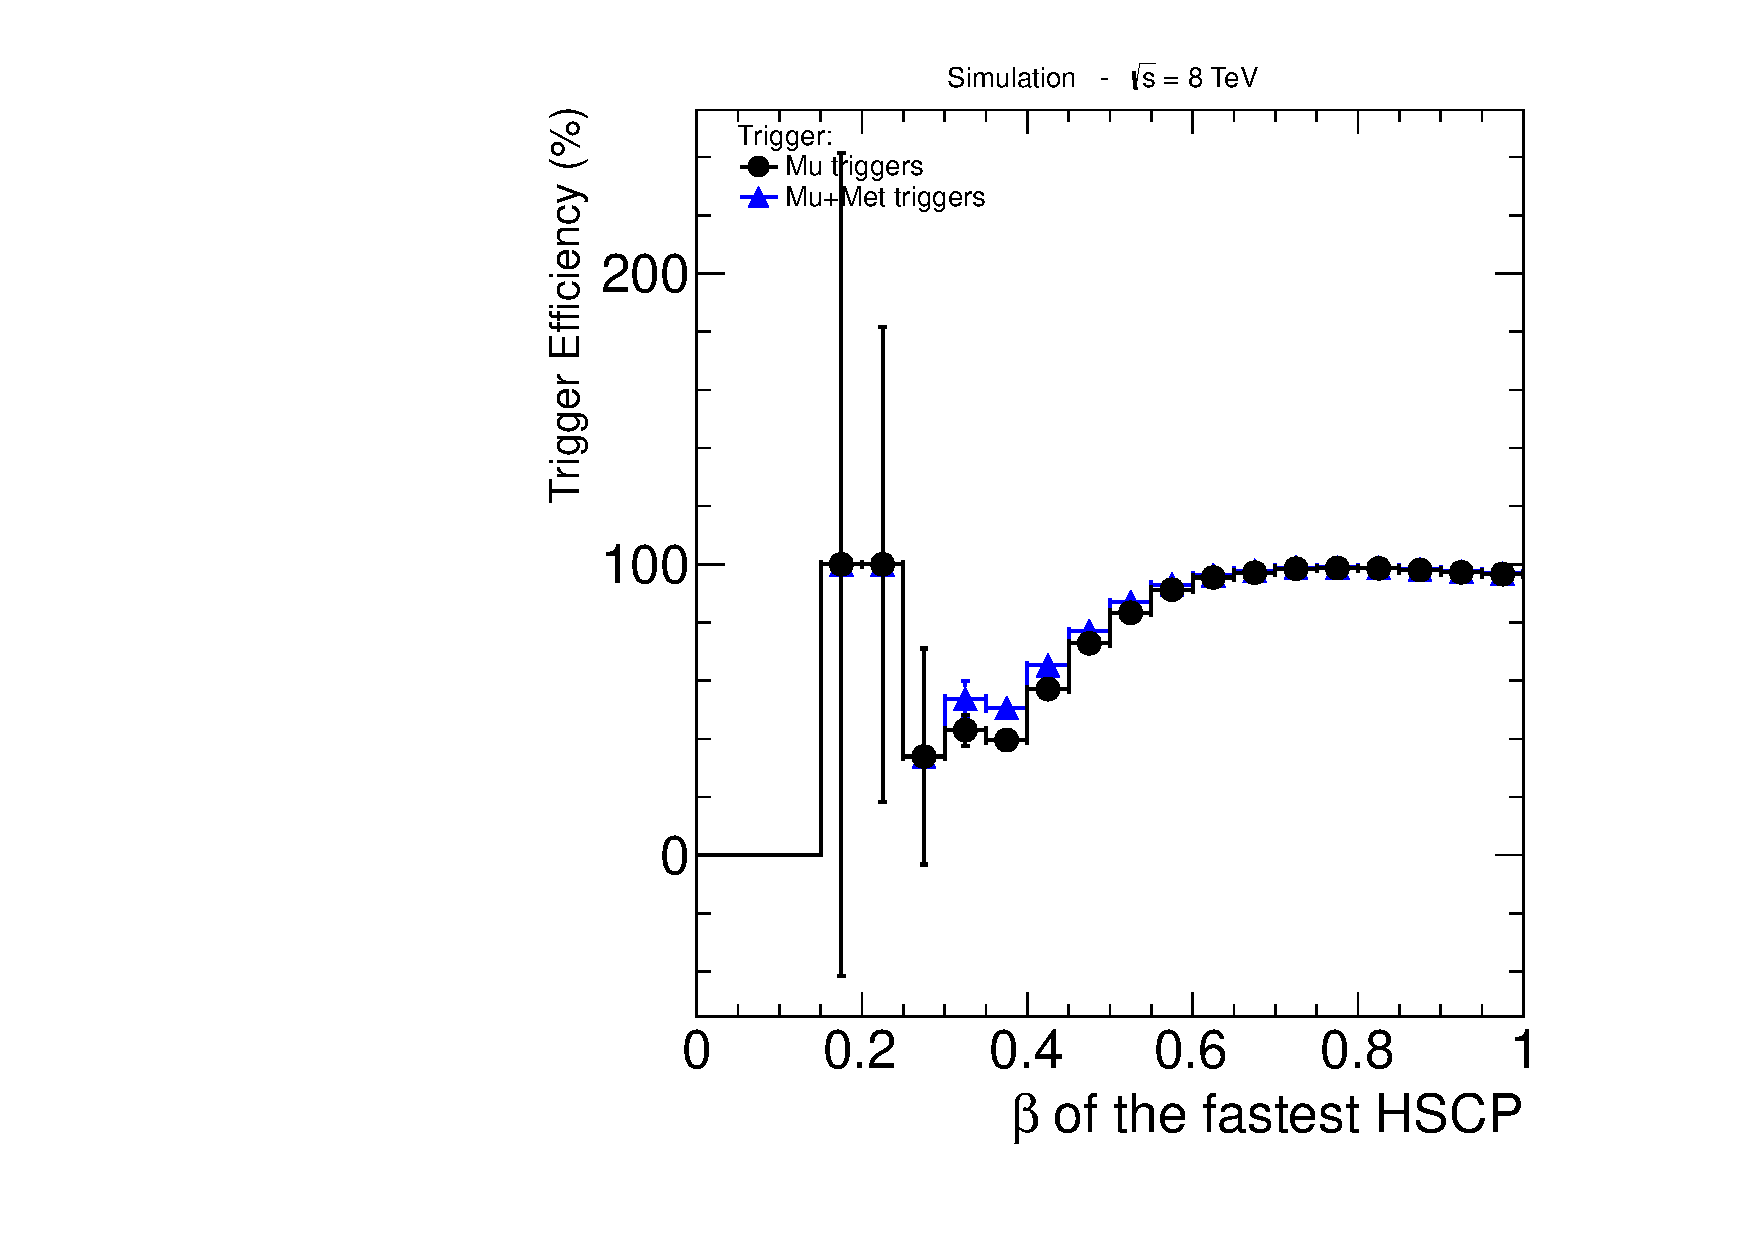
\includegraphics[clip=true, trim=0.0cm 0cm 3.0cm 0cm, width=0.32\textwidth]{figures/search/GMStau_8TeV_M494MatchedGl}
      \caption[Trigger efficiency as a function of the $\beta$ of the fastest HSCP reconstructed offline in the muon system with only the muon triggers
and additionally including the PFMET trigger.]
{Trigger efficiency as a function of the $\beta$ of the fastest HSCP reconstructed offline in the muon system with only the muon triggers
and additionally including the PFMET trigger.
Sample is 1200~GeV Gluino $f=0.1$ (left) and 800~GeV stop (right)}
    \label{fig:TriggerEffVsBetaGl}
\end{figure}

When evaluating trigger efficiencies, it is important to only consider events that have a possibility of being selected offline.
For the case of strongly charged HSCP this is made more difficult as some events may not have any $R-hadrons$ electrically charged while they pass through the detector.
To deal with this, the trigger efficiencies are reported with respect to events where at least one HSCP is found offline.
The efficiency for each trigger as well as the combined efficiency is listed for various signals in Tables~\ref{tab:triggEffSA} and ~\ref{tab:triggEffGl} in events
with at least one HSCP reconstructed in the muon system and muon system plus tracker, respectively.

\begin{table}
 \begin{center}
  \caption[Trigger efficiency for various models considered with respect to events with a reconstructed HSCP in the muon system]
{Trigger efficiency for various models considered using the SingleMu, PFMET, L2Mu+MET or a combination of the three.
Efficiencies with respect to events with at least one HSCP reconstructed in the muon system.}
     \label{tab:triggEffSA}
  \begin{tabular}{|l|c|c|c|c|c|} \hline
      Model     & Mass (GeV) & Mu40       & PFMET150   &  L2Mu+MET  & Total                 \\ \hline
 Gluino $f=0.1$ &  400  & 35.55      & 19.41      & 34.28      & 58.56    \\
 Gluino $f=0.1$ &  800  & 31.63      & 22.57      & 31.21      & 54.88    \\
 Gluino $f=0.1$ & 1200  & 26.62      & 20.45      & 24.63      & 47.52    \\
 Gluino $f=1.0$ &  400  &  5.55      & 23.22      & 36.63      & 46.07    \\
 Gluino $f=1.0$ &  800  &  5.01      & 24.50      & 31.88      & 43.41    \\
 Gluino $f=1.0$ & 1200  &  3.69      & 20.62      & 23.62      & 35.45    \\
           Stop &  200  & 42.79      & 11.15      & 27.31      & 58.80    \\
           Stop &  500  & 42.07      & 19.79      & 31.13      & 61.21    \\
           Stop &  800  & 41.57      & 21.57      & 30.33      & 60.73    \\ \hline
  \end{tabular}
 \end{center}
\end{table}

\begin{table}
 \begin{center}
      \caption[Trigger efficiency for various models considered with respect to events with a reconstructed HSCP in both the muon system and inner tracker]
{Trigger efficiency for various models considered using the SingleMu, PFMET, or a combination of the two.
Efficiencies with respect to events with at least one HSCP reconstructed in both the muon system and inner tracker.}
     \label{tab:triggEffGl}
  \begin{tabular}{|l|c|c|c|c|} \hline
      Model     & Mass (GeV) & Mu40       & PFMET150   & Total                 \\ \hline
 Gluino $f=0.1$ &  400  & 51.87      & 16.06      & 59.09    \\
 Gluino $f=0.1$ &  800  & 46.50      & 20.50      & 56.42    \\
 Gluino $f=0.1$ & 1200  & 38.96      & 19.56      & 49.95    \\
 Gluino $f=1.0$ &  400  & 41.81      & 19.36      & 51.76    \\
 Gluino $f=1.0$ &  800  & 37.83      & 21.57      & 49.01    \\
 Gluino $f=1.0$ & 1200  & 31.70      & 21.16      & 45.21    \\
           Stop &  200  & 58.43      &  7.69      & 61.54    \\
           Stop &  500  & 56.91      & 17.40      & 64.44    \\
           Stop &  800  & 56.15      & 20.49      & 65.59    \\
      CD Stau &  100  & 97.86      & 14.74      & 98.06    \\
      CD Stau &  308  & 97.03      & 17.53      & 97.47    \\
      CD Stau &  494  & 95.56      & 17.76      & 96.35    \\
        DP Stau &  100  & 95.06      &  0.17      & 95.09    \\
        DP Stau &  200  & 95.78      &  0.37      & 95.82    \\
        DP Stau &  494  & 95.23      &  1.16      & 95.36    \\ \hline
  \end{tabular}
 \end{center}
\end{table}

Muons from cosmic rays are an important background for the \muononly\ analysis. To study and predict them a trigger that selects events when no beams are passing through
CMS is used. The trigger requires the presence of a muon system track with $p_T > 20$~GeV, no proton bunches passing through CMS within 50ns, and for the event not to be flagged as
noise from the LHC beams. The muon system track reconstruction used for the cosmic ray muon trigger is slightly 
different than for the collision trigger as it is not updated at vertex,
the meaning of this is discussed in section~\ref{sec:preselection}. However, both reconstructions are required offline so no bias is introduced.

\section{Selection Variables \label{sec:SelVar}}
HSCPs can be distinguished from SM particles in CMS due to their high momentum and slow speed.
The momentum of a particle can be determined by its bending in the magnetic field of CMS.
The slow speed of HSCPs lead to two interesting detector signatures. The first is that the particles will arrive at the detector elements later than SM particles will.
The muon system, being the furthest detector element from the interaction point, has the largest timing difference. The measurement of the arrival time of particles in the
muon system is discussed in Ch.~\ref{sec:timing}. The \invbeta\ variable is used in the searches to discriminate between HSCPs and SM particles.
The second interesting signature is that HSCP have a larger amount of ionization energy loss per unit length 
than SM particles of the same momentum as discussed below.

\subsection{Transverse Momentum Measurement \label{sec:PMeasurement}}
A muon passing through CMS will likely be reconstructed three times~\cite{2012JInst...7P0002T}; once only in the silicon tracker, referred to as a tracker track;
once only in the muon system, referred to as a stand-alone muon; and once as a combined track found in both the muon system and silicon tracker, referred
to as a global muon. CMS measures the curvature of a track which is proportional to and can be used to determine the $Q/p_T$ of the track.
In the central region of CMS, tracker tracks have a resolution on $Q/p_T$ of 1\% for muons at intermediate momentum and 7\% at
high momentum with the resolution being approximately
twice as large in the forward region. Intermediate momentum is defined as 15--100~GeV and high momentum is defined as 400--1000 GeV.
Stand-Alone muons in the central region have a resolution on $Q/p_T$ of 8\% for intermediate momentum and 25\%~\cite{2008AN097} for high momentum with the uncertainty again
being about twice as large in the forward region. The resolution for global muons is the same as for tracker muons for intermediate momentum and is slightly better
than tracker muons at high momentum at 6\% in the central region.

The \muononly\ analysis uses the $p_T$ measurement coming from the stand-alone muon while the rest of the analyses use the measurement from the tracker track.
The tracker track momentum is used even when the global muon is available due to issues specific to $R$-hadrons.
$R$-hadrons are unlikely to undergo a nuclear interaction while traversing the silicon tracker so they would have the same electric charge at all points in the tracker.
While passing through the muon system however, $R$-hadrons will often undergo a nuclear interaction with the steel return yoke located between the muon stations
possibly causing the electric charge to change in the middle of the muon system. This behavior affects the momentum measurement of the HSCP track in the muon system.

To convert the measured $Q/p_T$ to $p_T$, a charge of $Q=1e$ is assumed.
For $R$-hadrons that can change their charge inside of CMS it can be the case that the average value of $Q$ during their passage through the muon system does not equal $1e$.
This effect has different consequences for the stop and gluino samples.

A stop particle, specifically not an anti-stop, has a charge of $+(2/3)e$ and forms an $R$-hadron with either an anti-quark ($\tilde{t} \bar{q}$) or
two quarks  ($\tilde{t} q q$). Anti-quarks have a charge of $-(2/3)e$ or $+(1/3)e$ leading to $R$-hadrons with a charge
of either 0 or $+1e$. Quarks have a charge of either $+(2/3)e$ or $-(1/3)e$ which allows for
the creation of $R$-hadrons with a charge of 0, $+1e$, or $+2e$. Thus a stop $R$-hadron will always have a
positive charge or be neutral. For an anti-stop, the effect is reversed and the $R$-hadron will always have a
negative charge or be neutral.

For gluino $R$-hadrons this statement does not hold true. Gluinos can hadronize into glue balls ($\tilde{g}g$), $R$-mesons ($\tilde{g} q \bar{q}$), or
$R$-baryons  with either quarks or anti-quarks ($\tilde{g} qqq$ or $\tilde{g} \bar{q}\bar{q}\bar{q}$),
allowing the charge of the $R$-hadron to range from $-2e$ to $+2e$. This leads to the
average charge of the $R$-hadron as it traverses the muon system to often be less than $1e$ and the $p_T$ value to be overestimated allowing for further separation
between HSCP and SM particles.

To observe this effect the function
$\Delta(Q/p_T)$ is defined in Equation~\ref{eq:deltaqopt}
\begin{equation}
\Delta(Q/p_T) = ((Q/p_T)_{SA} - (Q/p_T)_{Tk})/(Q/p_T)_{Tk}
\label{eq:deltaqopt}
\end{equation}
where ``SA'' refers to stand-alone muon qualities and ``Tk'' refers to
tracker track qualities. As the $p_T$ resolution of tracker tracks is much better than for stand-alone muons, it is a sufficiently good approximation
of the true particle momentum. Figure~\ref{fig:MuOnlyInvPtDiff} shows the distribution of
$\Delta(Q/p_T)$ for tracks with inner track $p_T > 200$ GeV
for data and various simulated HSCP signal samples.
A value of zero in this plot indicates the $p_T$ was reconstructed correctly
while negative one indicates the reconstructed $p_T$ approaches infinity.
The CD stau sample, which does not change charge,
has a distribution similar to data, though slightly wider.
The slight discontinuity at negative one is due to particularities of the reconstruction but only affects a small number of tracks.
The stop sample, which is not able to flip charge but merely to switch
between one sign and zero, is centered at zero but with a slightly wider
width than data or CD stau.
The gluino sample, which can flip charge, is centered closer to negative one meaning that
the reconstructed $p_T$ is normally larger than what is generated, sometimes
to a very large degree. This increases the differences between gluino HSCPs and the background.

\begin{figure}
 \begin{center}
  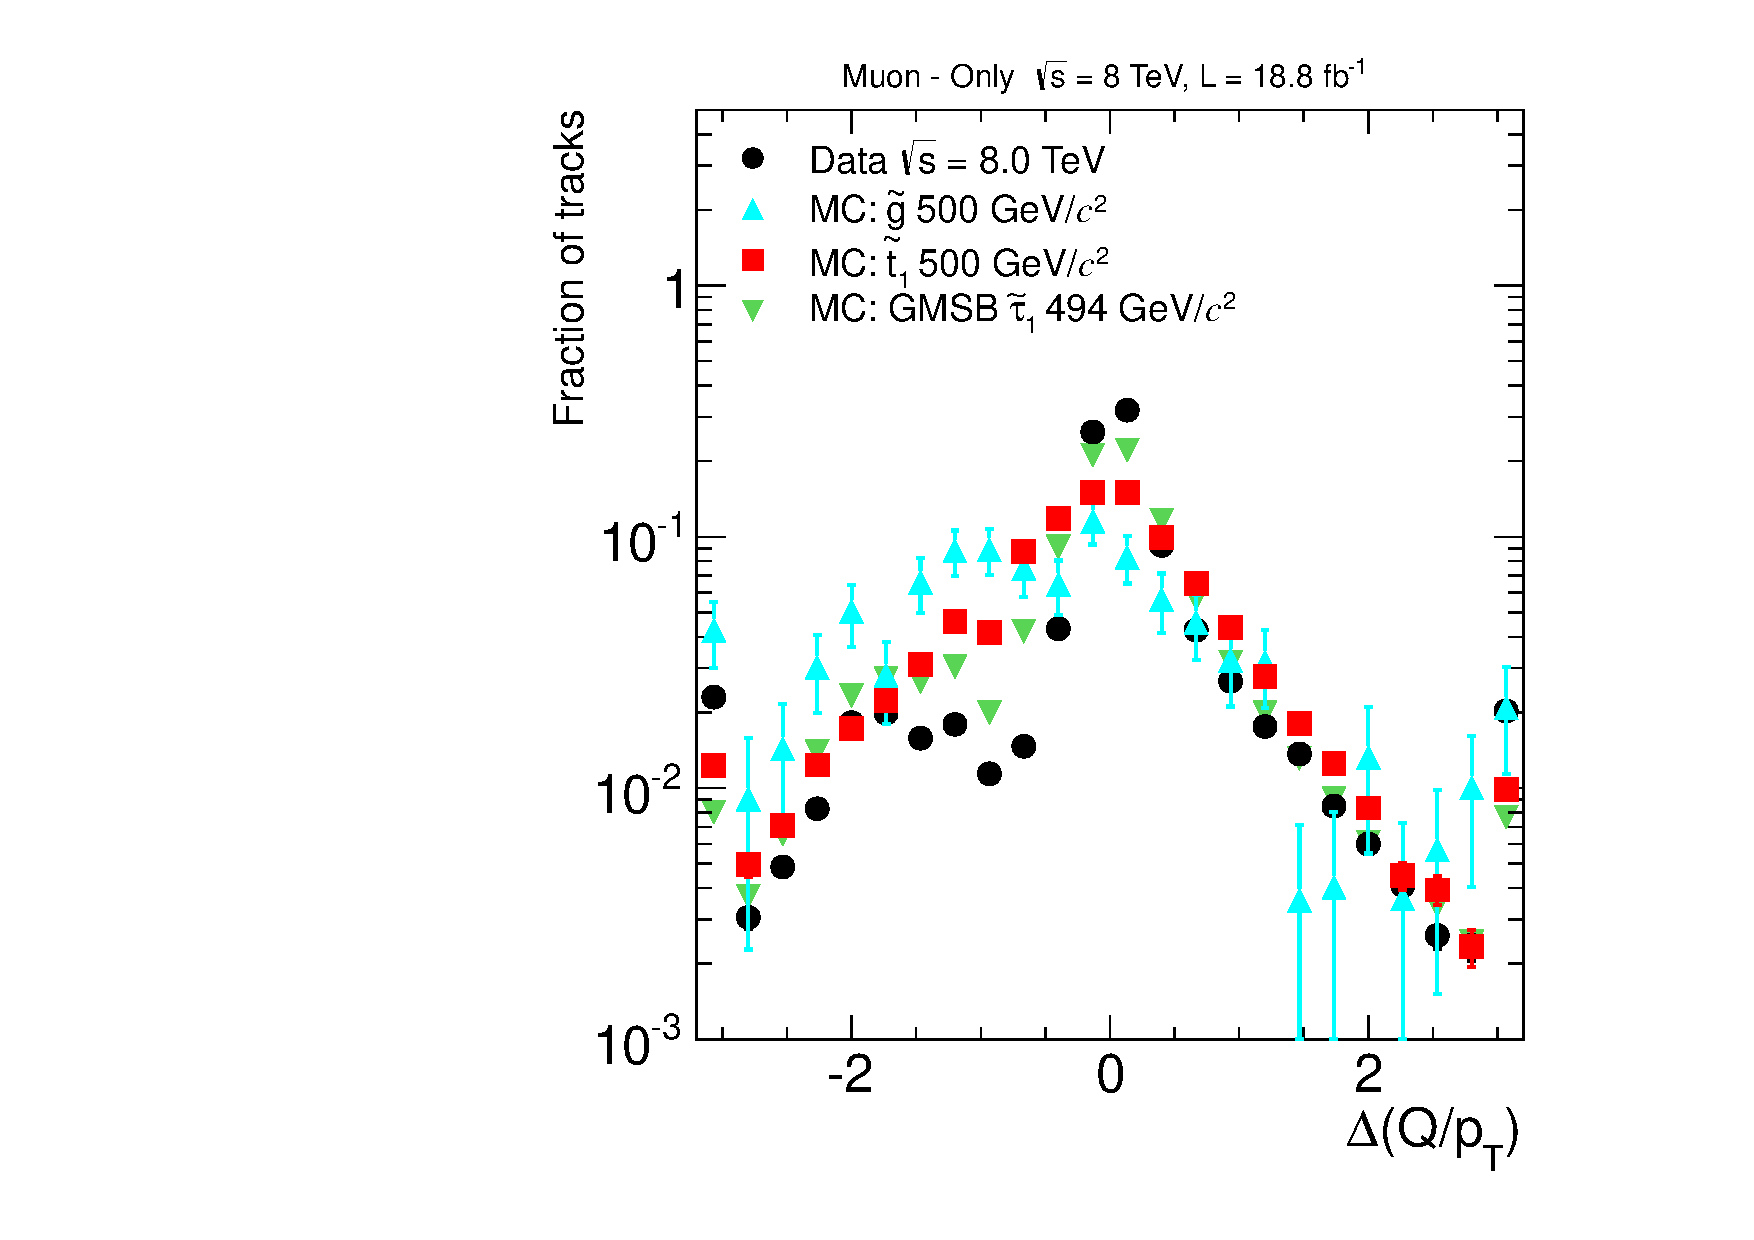
\includegraphics[width=0.44\textwidth]{figures/muonly/Selection_Comp_Signal_8TeV_InnerInvPtDiff_BS}
 \end{center}
 \caption{Distribution of $\Delta(Q/p_T)$
    for data, 500 GeV gluino, 500 GeV stop, and 494 GeV CD stau.
    \label{fig:MuOnlyInvPtDiff}}
\end{figure}

For the lepton like samples with non-unit charge, the \pt\ will be mismeasured by a factor of $1/Q$. This means that multiply 
charged particles will have their \pt\ underestimated making them somewhat harder to separate from backgrounds.
This effect can be seen in Figure~\ref{fig:RecoGenPt}.
%For the lepton like samples with non-unit charge the \pt\ will be mismeasured by a factor of 1/Q, meaning fractionally charged particles will have their \pt\ overestimated
%while multiply charged particles will be underestimated. This effect can be seen in Figure~\ref{fig:RecoGenPt}.

\begin{figure}
 \begin{center}
  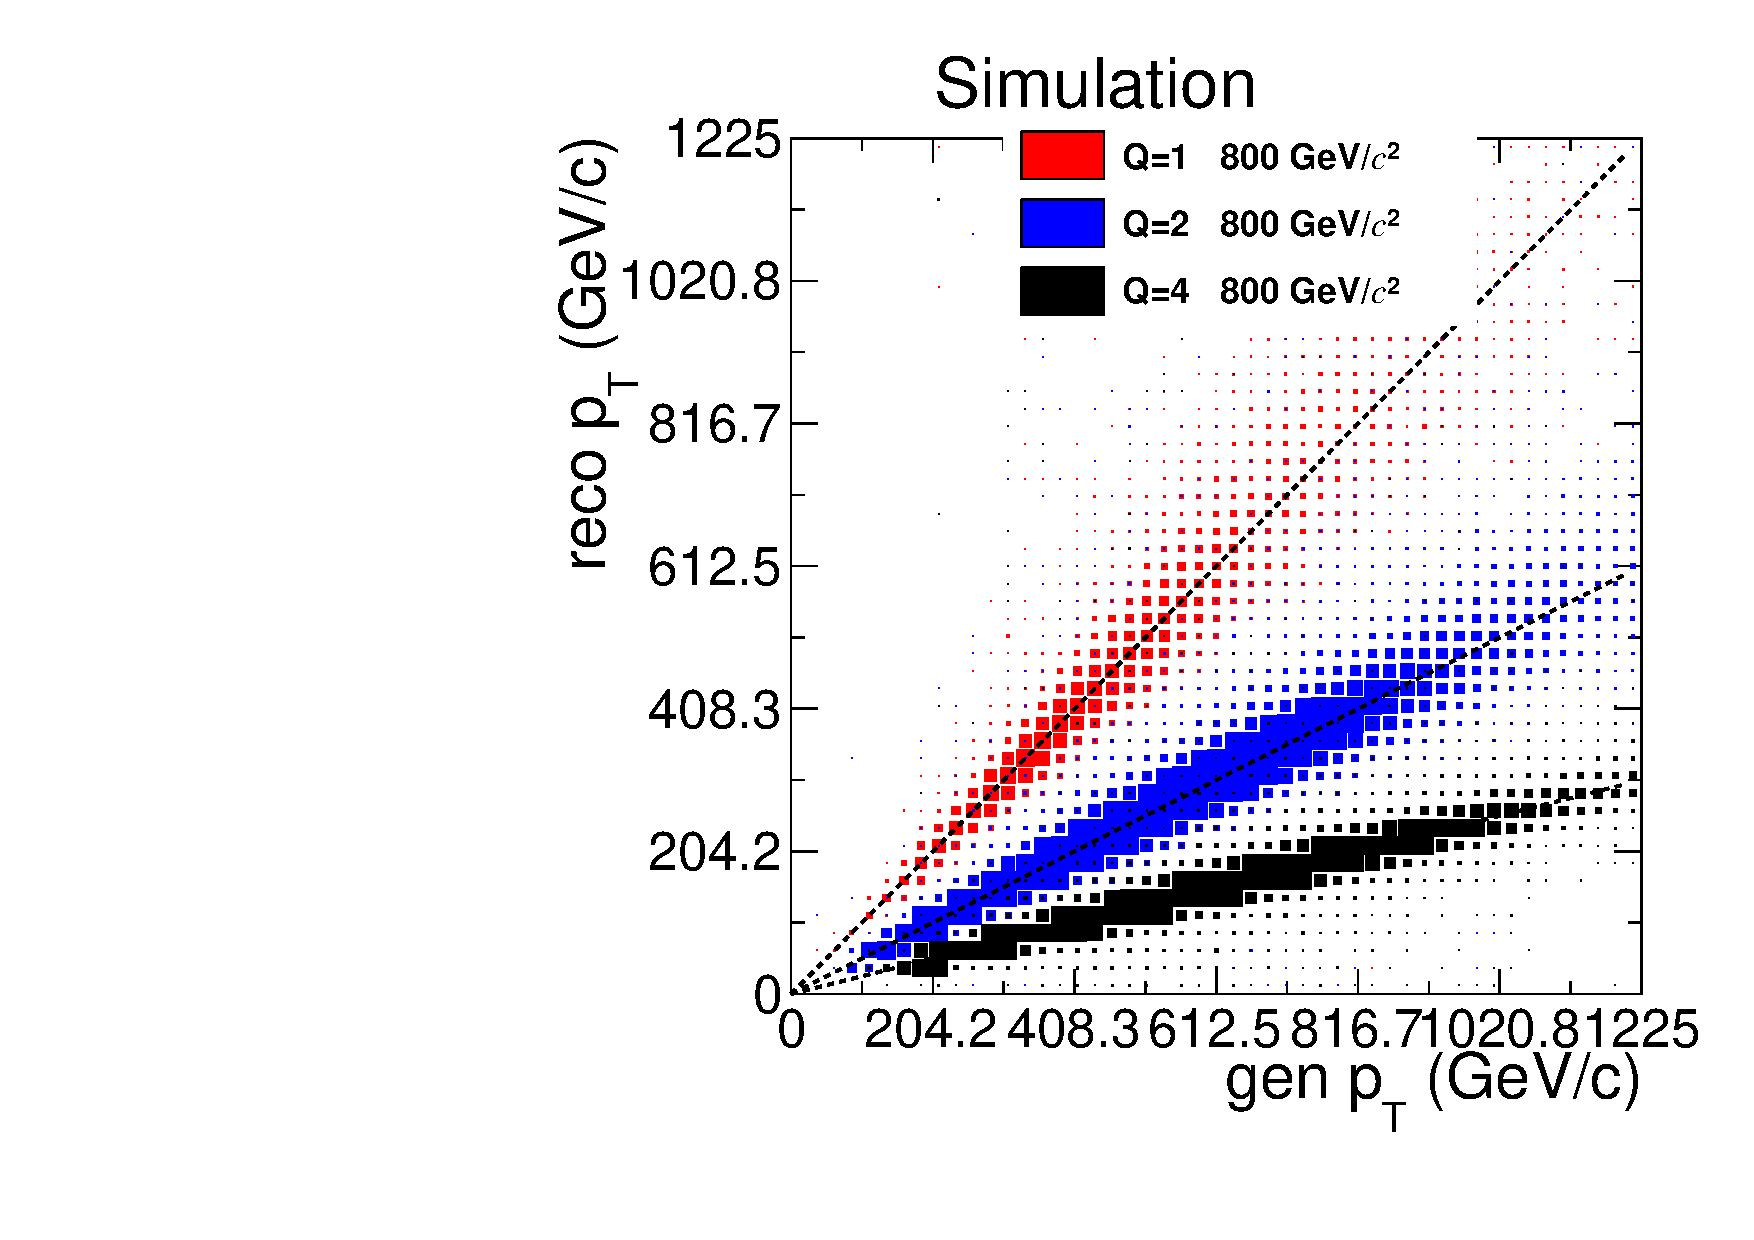
\includegraphics[width=0.44\textwidth]{figures/tkonly/SIM_Validation_Pt.pdf}
 \end{center}
 \caption{Distribution of reconstructed $p_T$ versus generator $p_T$ for Q=1e, 2e, and 4e samples.
    \label{fig:RecoGenPt}}
\end{figure}

\subsection{Energy Loss Measurement \label{sec:DedxMeasurement}}
The amount of ionization energy a particle deposits can be measured by the silicon tracker.
%that a slow moving HSCP will have a larger ionization energy loss in the silicon tracker than SM particles will.
For paticles with 0.1 $\gtrsim \beta \gamma \lesssim$ 1000, where $\gamma$ is $1/\sqrt{1 - \beta^2}$,
the average amount of the ionization energy deposited per unit length in a given material, \dedx, is to a large degree dependent only on the velocity of the particle
and its charge as described by the Bethe-Bloch formula~\cite{PDG}.
The dependence of \dedx\  on charge varies approximately as $Q^2$, meaning that even a $Q=2e$ HSCP will have almost four times as much energy loss as a SM particle. 
The dependence on speed for particles with $0.1 < \beta < 0.9$ varies approximately as $1/\beta^2$; so slow moving HSCP would have large \dedx\ values.
At higher speeds, the energy loss has a broad minimum up to $\beta \gamma$ of 1000.
Particles in this broad minimum all have close to the same energy loss and are generically referred to as minimum ionizing particles (MIP).
Above this level, radiative effects become important as they cause very rare, very high-energy losses that result in an increase to the average energy loss.
Techniques described below are used to help mitigate the effect of this radiative rise.
%Experimental techniques are used to reduce the impact of these rare high-energy losses so that
%SM particles with a momentum above 10~GeV will all have mean \dedx\ close to the minimum value
%($\approx$ 3MeV/cm) and are referred to as minimum ionizing particles (MIPs).

A short description of the \dedx\ measurement is included here, a more detailed description can be found in~\cite{2010EPJC...70.1165K, Khachatryan:2011ts, Quertenmont:1361029}.
As in~\cite{Chatrchyan:2012sp}, two variables related to \dedx\ are calculated for each track. 
The first is a harmonic mean of the \dedx\ measurements along the track;
\begin{equation}
 I_h= \biggl( \cfrac{1}{N} \sum_i c_{i}^{-2} \biggr)^{-1/2},
 \label{eq:HarmonicEstimator}
\end{equation}
where $N$ is the number of measurements in the silicon-strip tracker and $c_{i}$ is the energy loss per unit path length
of the $i$th measurement. The use of a harmonic mean greatly reduces the impact of the rare radiative losses as the highest energy
losses are effectively given less weight than lower energy losses. This leads to all
SM particles produced at the LHC with momentum above 10~GeV on average having \ih\ values close to the minimum value ($\approx$ 3MeV/cm). 
HSCP will have high \ih\ as their energy loss is consistently large.

The second variable is \ias\ which is a modified version of the Smirnov-Cramer-von Mises~\cite{Eadie, James} discriminant.
The discriminant is given by:
\begin{equation}
 I_{as} = \frac{3}{N} \times \left(
   \frac{1}{12N} + \sum_{i=1}^N
   \left[
   P_i \times \left( P_i - \frac{2i-1}{2N} \right)^2 \right] \right),
\end{equation}
where $P_i$ is the probability for a MIP to
produce a charge smaller or equal to that of the $i$th measurement in the silicon-strip tracker
for the observed path length in the detector, and the sum is over the
measurements ordered in terms of increasing $P_i$. The probabilities are found from tracks with momentum greater than five~GeV collected with a trigger requiring only
that a proton collision occured inside CMS. The discriminant is designed to give the best separation between MIPs and high-ionizing particles.
The discriminant is peaked at zero for MIPs and approaches one for high-ionizing particles.
The same measurements are used to determine \ih\ and \ias\ so the variables are not independent. 

An estimate of the mass $m$, assuming Q=1$e$, of a particle can be made from \ih\ and the momentum $p$ of a track. This is done by using Eq.~\ref{eq:MassFromHarmonicEstimator};
\begin{equation}
I_h= K\cfrac{m^2}{p^2}+C.
\label{eq:MassFromHarmonicEstimator}
\end{equation}
with  $K=2.559 \pm 0.001$ MeV cm$^{-1}$ $c^2$ and $C=2.772 \pm 0.001$ MeV cm$^{-1}$ as determined from low momentum protons~\cite{Khachatryan:2011ts}.


\section{Preselection \label{sec:preselection}}
Candidates for the \muononly\ analysis are tracks identified as stand-alone muons. Candidates for the \tktof\ and \multi\ analyses are tracks identified
as global muons. The candidates for the \tkonly\
%and fract\ analyses require  
analysis are tracks found in the silicon tracker.
Various requirements are applied to the candidates in order to reduce tracks from background processes while maintaining good efficiency for HSCP.
%For all plots shown in this section the first and last bins contain the underflow and overflow, respectively.

\subsection{Preselection for \muononly\ \label{sec:muonlypreselection}}

The \muononly\ analysis requires the tracks to have $p_T > 80$~GeV, $|\eta| < 2.1$, and valid DT or CSC hits in at least two muon stations
to reinforce the requirements applied at trigger level. 
The distributions of $\eta$ and number of muon stations are shown in Fig.~\ref{fig:MuOnlyPreselA} for data, the cosmic-ray muon control sample, and signal MC samples.
The discontinuities in the $\eta$ distribution are due to interfaces between the detector elements in the muon system.

Quality cuts on the \invbeta\ measurement are applied. The measurement must have at least eight degrees of freedom and the uncertainty must be less than 0.07.
Additionally the track must have \invbeta\ greater than one.
A potential background source is muons coming from adjacent bunch crossings.
Tracks are required to have a measured time at vertex not be within $\pm5$~ns of an expected adjacent collision.
Figure~\ref{fig:MuOnlyPreselB} shows the distribution of these quantities for data, cosmic-ray muon control sample, and signal MC samples.

Additional cuts are used to control the background from cosmic-ray muons. Tracks are vetoed if the displacement of the track
with respect to the beam spot is larger than 15~cm in either the longitudinal or transverse direction relative to the beam line. 
The track $|\phi|$ must not be within 1.2--1.9 radians, this region represents tracks pointing in the vertical
direction, as is expected of cosmic-ray muons. Cosmic-ray muons travel 
through the top and bottom halves of the detector leaving hits in the muon system opposite of the track.
Thus, it is required that  there be no muon segments with $\eta$ within 0.1 of $-\eta_{track}$. The requirement is only applied to 
segments separated from the track by at least 0.5 in $\phi$ so that tracks with $\eta$ close to zero do not match to their own segments.
Figure~\ref{fig:MuOnlyPreselC} shows the distribution of these quantities.

\begin{figure}
\centering
  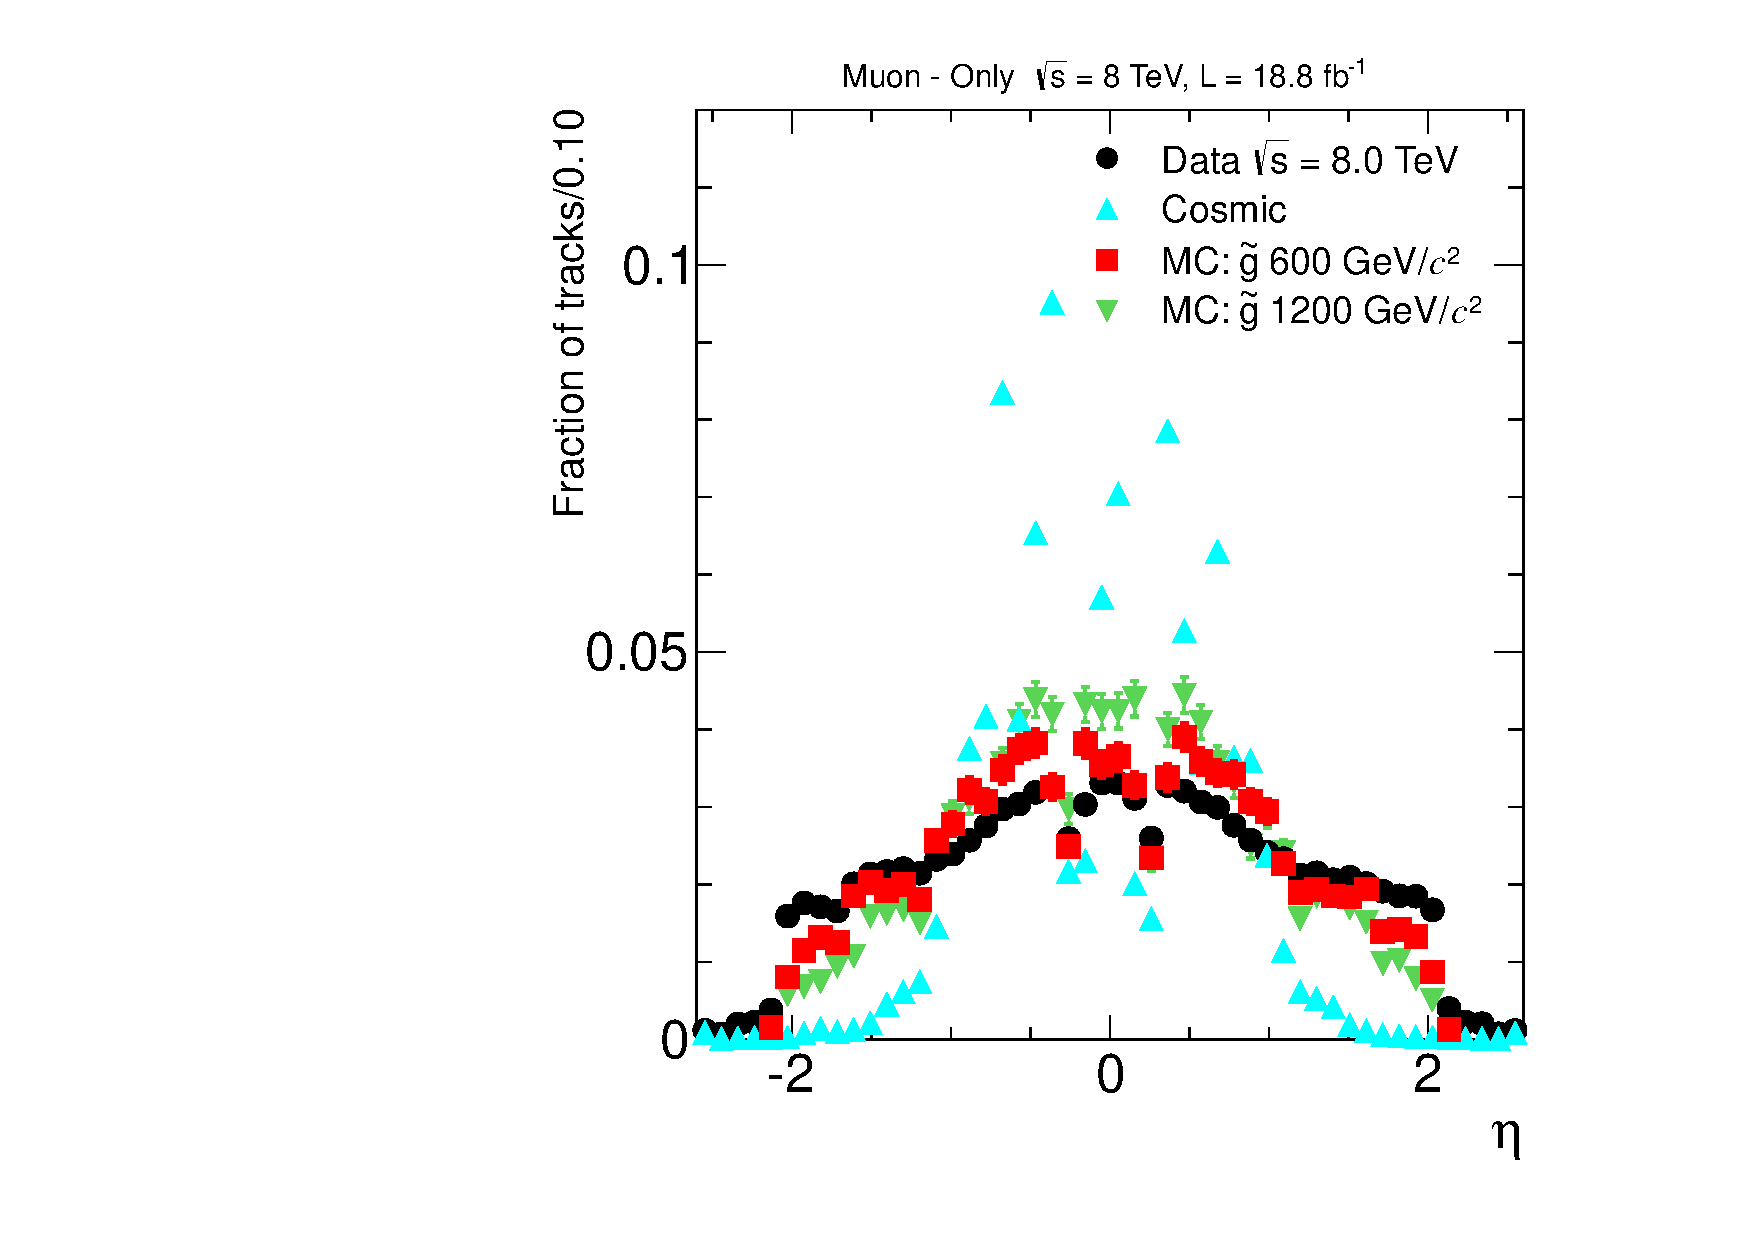
\includegraphics[clip=false, trim=0.0cm 0cm 0.0cm 0cm, width=0.48\textwidth]{figures/muonly/Selection_Comp_8TeV_Cosmic_Eta_BS}
  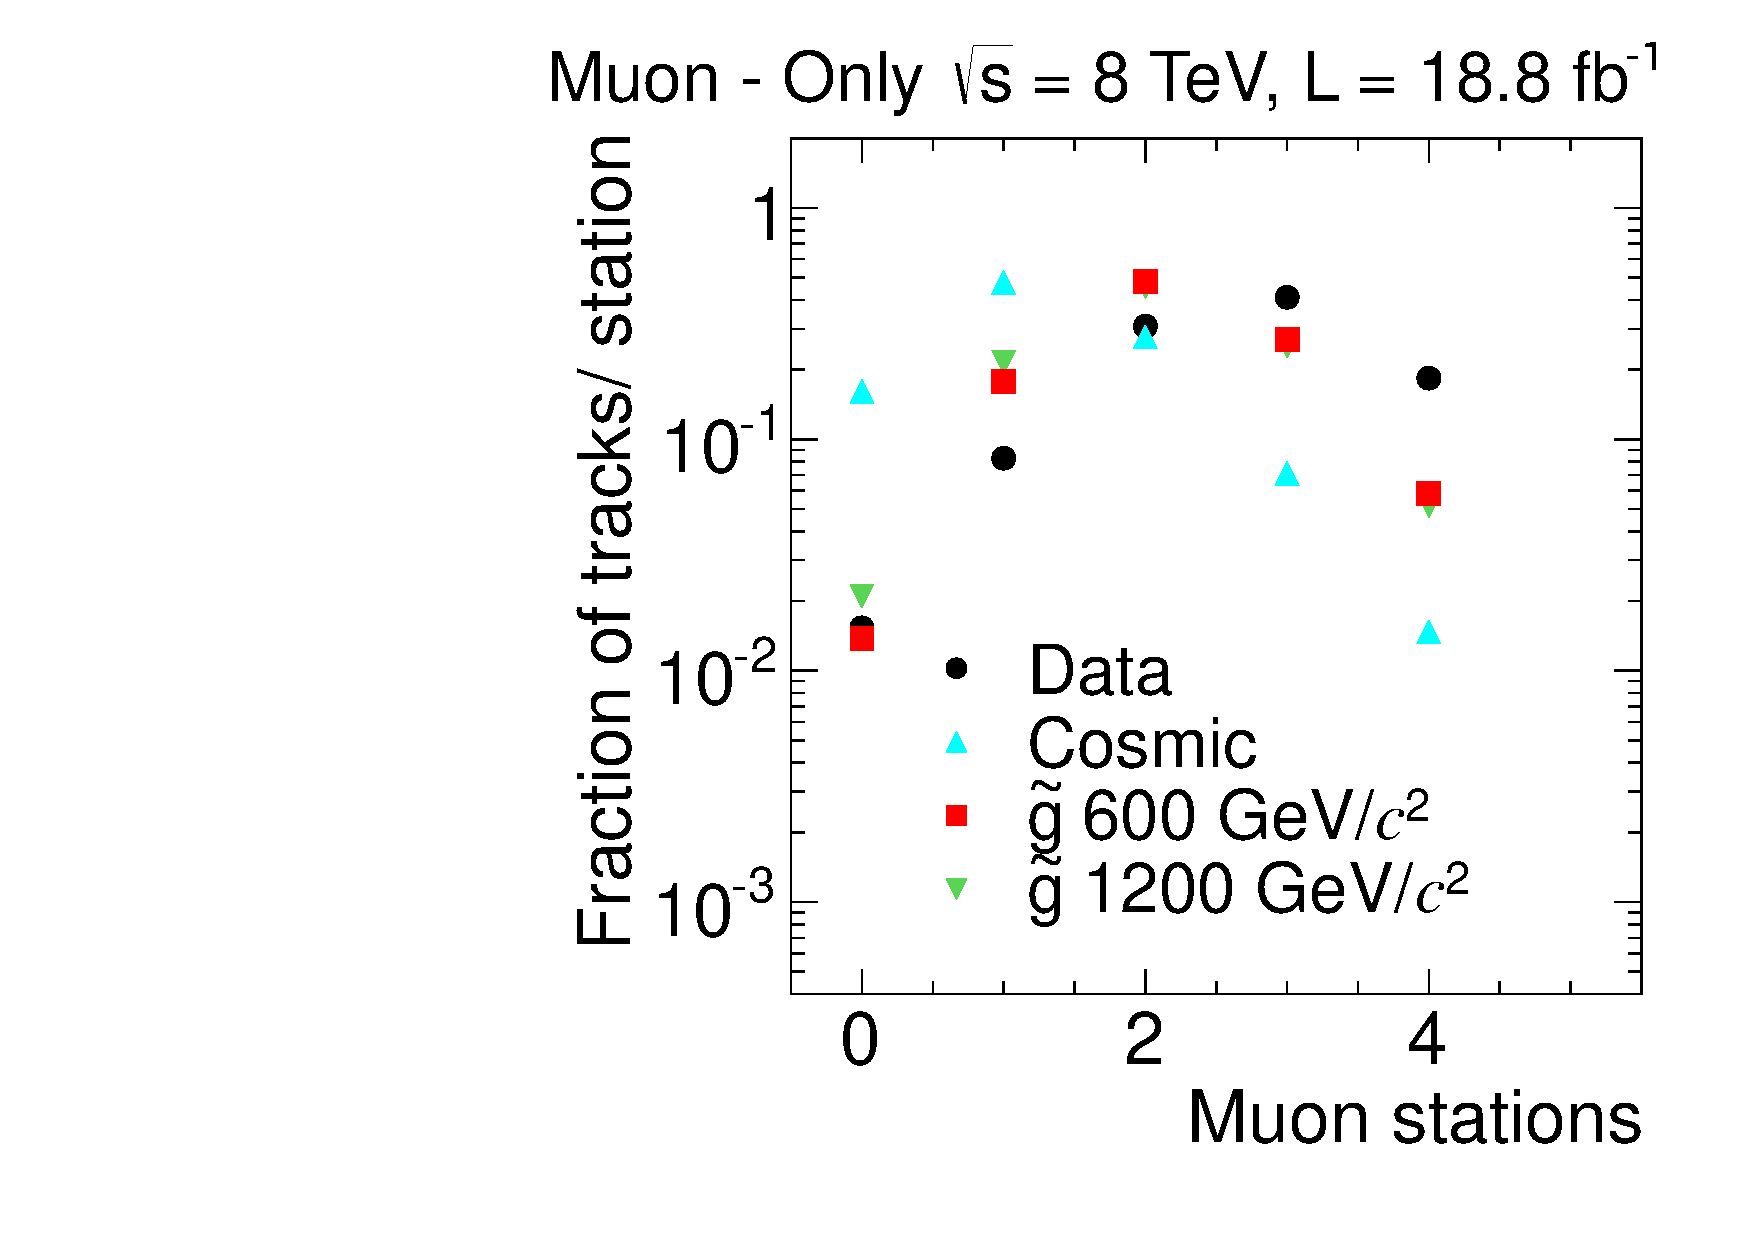
\includegraphics[clip=false, trim=0.0cm 0cm 0.0cm 0cm, width=0.48\textwidth]{figures/muonly/Selection_Comp_8TeV_Cosmic_MatchedStations_BS} \\
\caption[Distribution of $\eta$ and number of matched muon stations for data, cosmic-ray muon control sample, and signal MC samples in the \muononly\ analysis.]
{Distribution of $\eta$ (left) and number of matched muon stations (right) for tracks in the \muononly\ analysis
for data, cosmic-ray muon control sample, and signal MC samples.}
    \label{fig:MuOnlyPreselA}
\end{figure}

\begin{figure}
\centering
  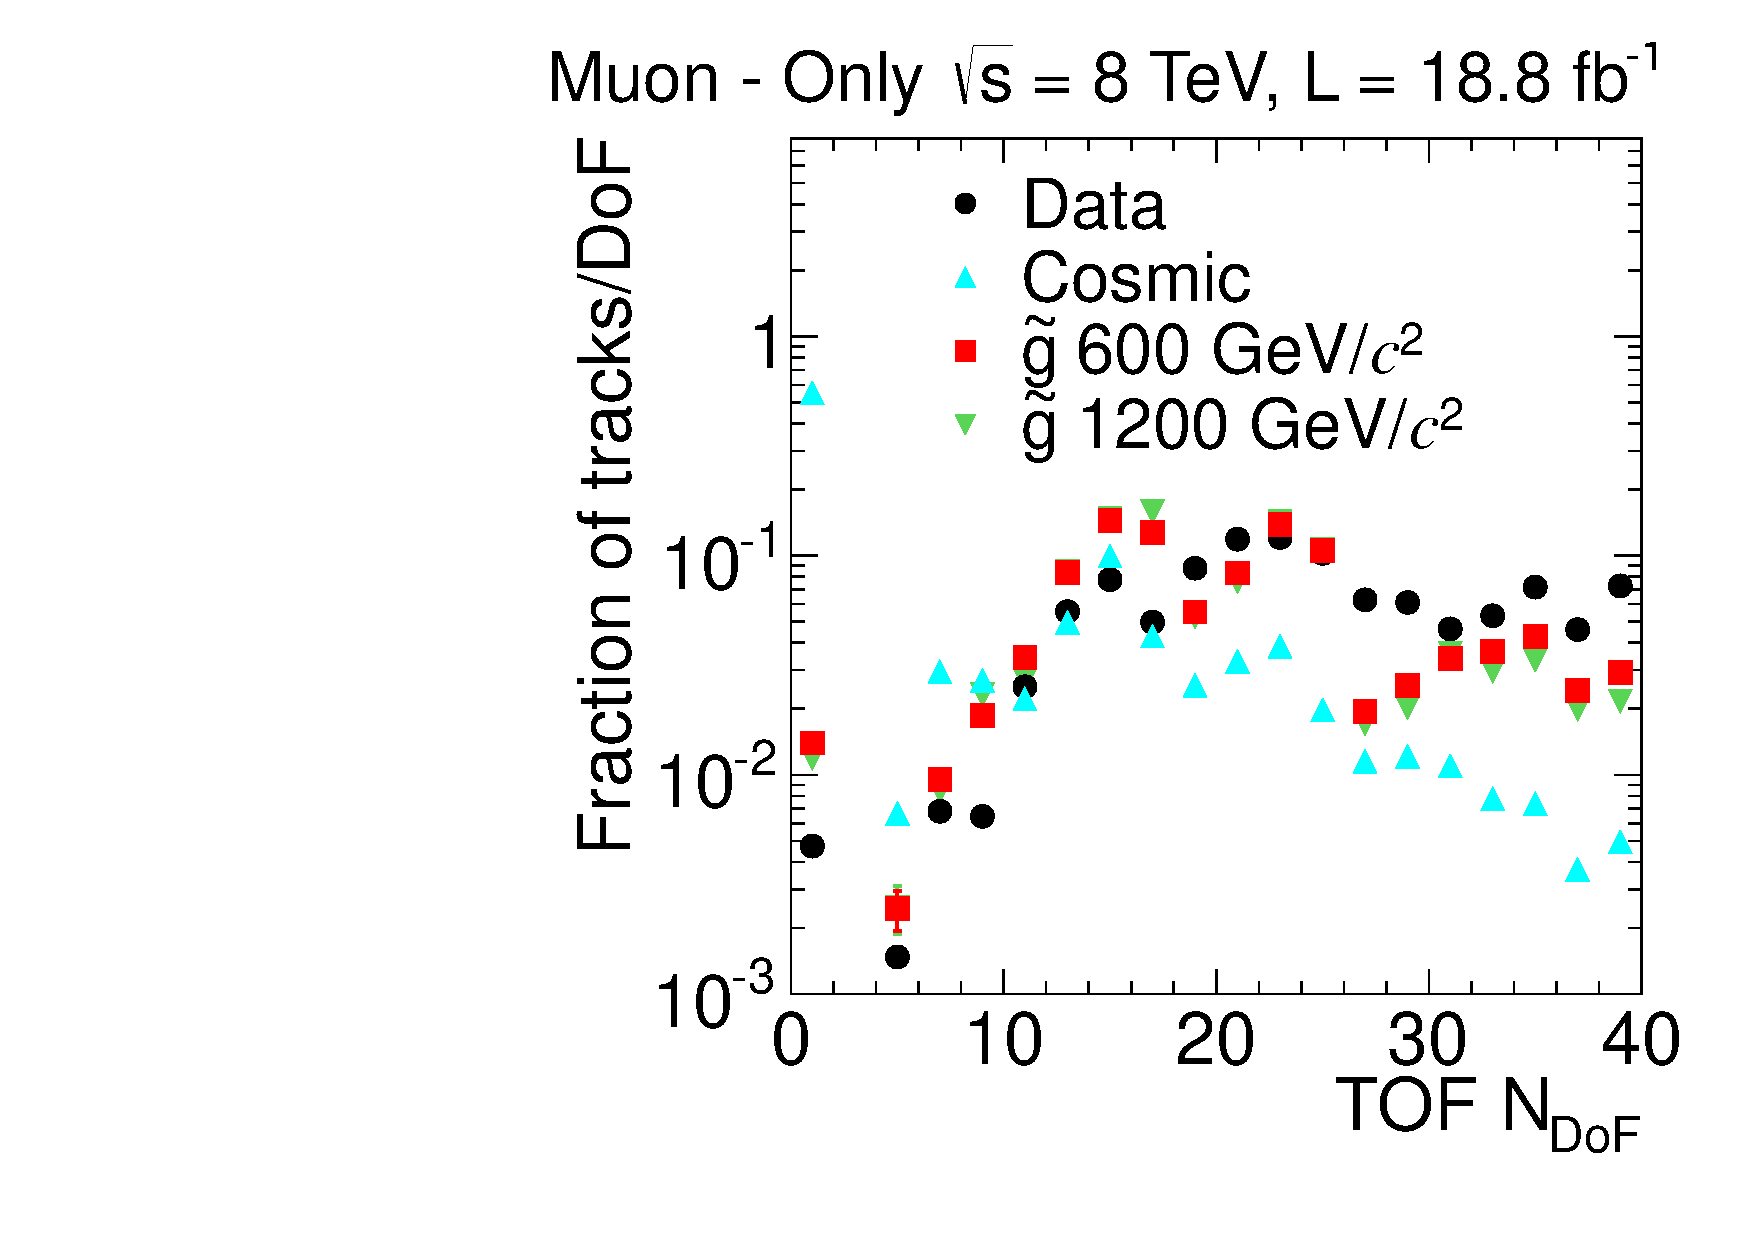
\includegraphics[clip=false, trim=0.0cm 0cm 0.0cm 0cm, width=0.48\textwidth]{figures/muonly/Selection_Comp_8TeV_Cosmic_nDof_BS}
  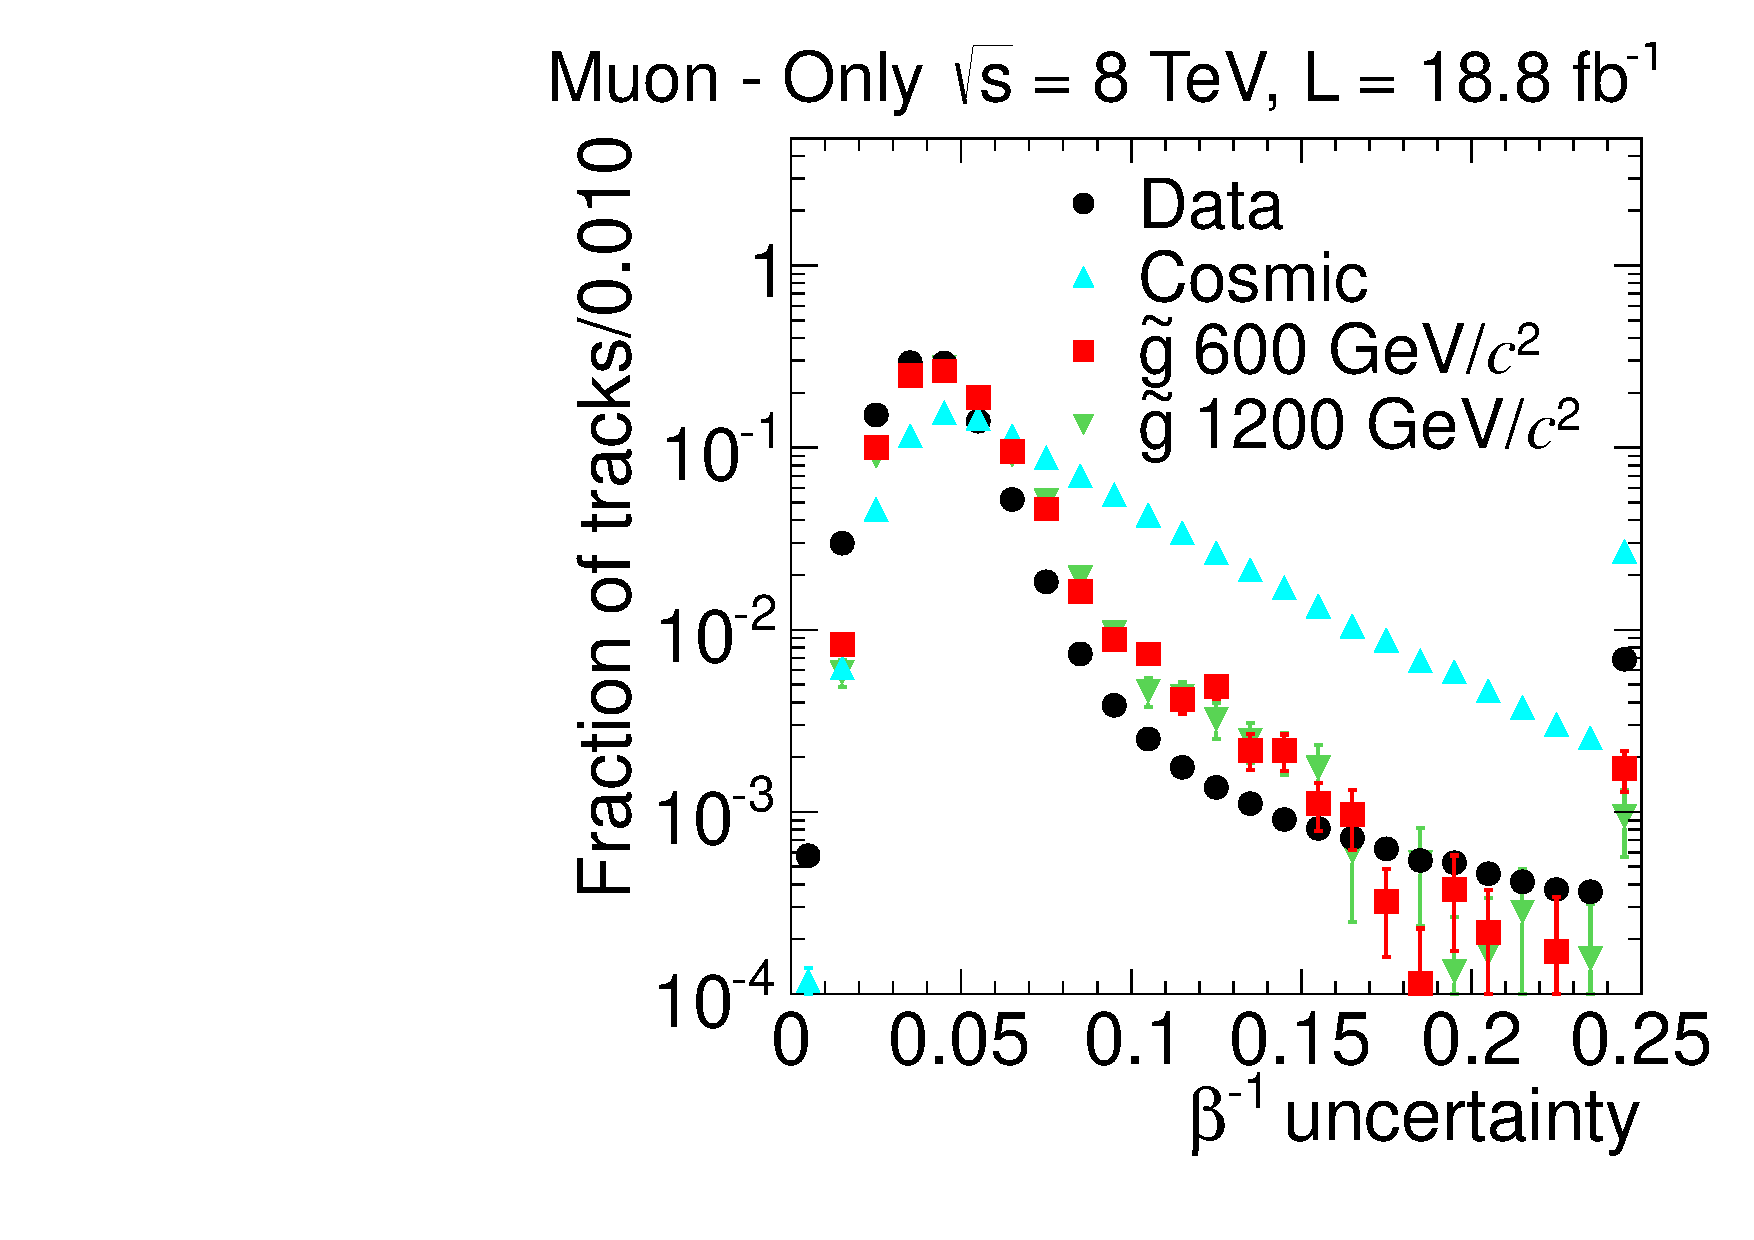
\includegraphics[clip=false, trim=0.0cm 0cm 0.0cm 0cm, width=0.48\textwidth]{figures/muonly/Selection_Comp_8TeV_Cosmic_TOFError_BS} \\
  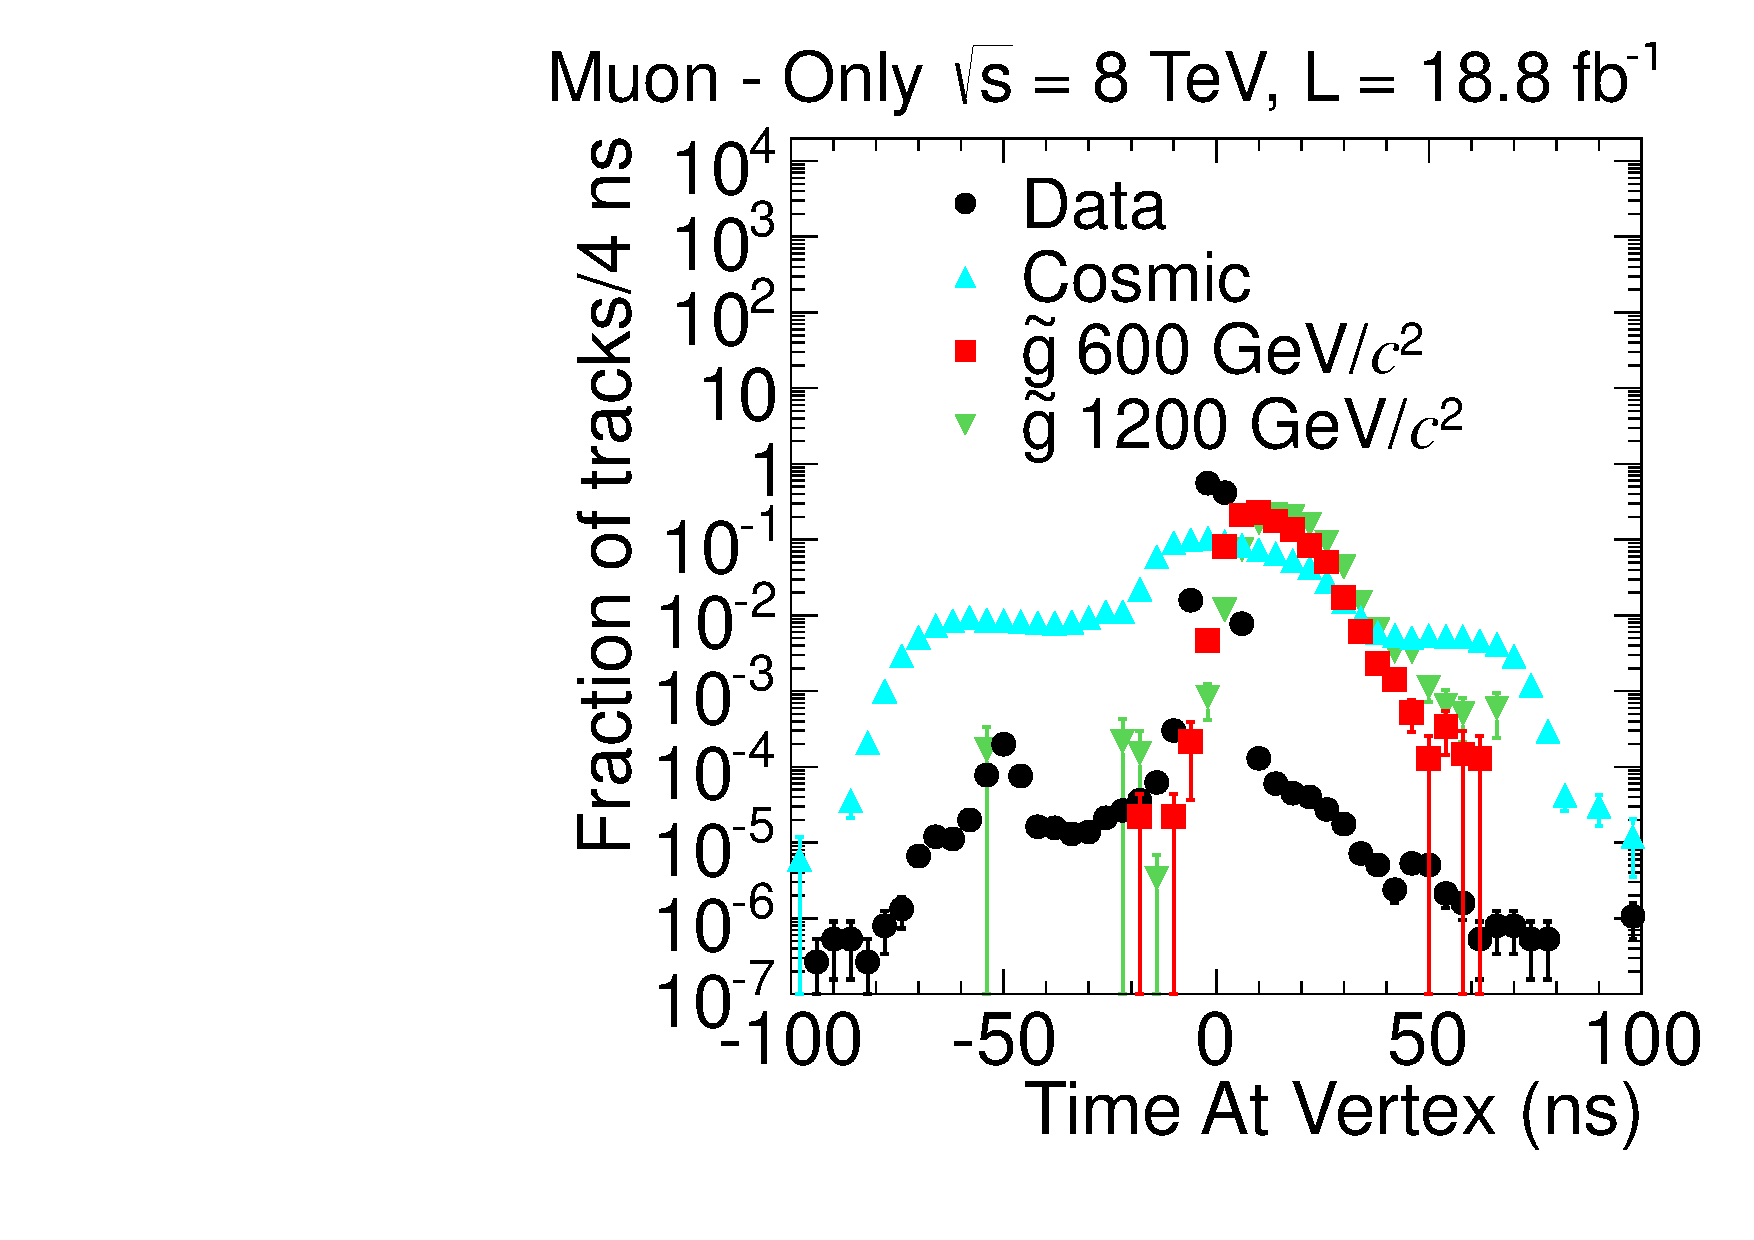
\includegraphics[clip=false, trim=0.0cm 0cm 0.0cm 0cm, width=0.48\textwidth]{figures/muonly/Selection_Comp_8TeV_Cosmic_TimeAtIP_BS} \\
\caption[Distribution of number of degrees of freedom (left) and uncertainty (right) on the \invbeta\ measurement and time at vertex in 
the \muononly\ analysis for data, cosmic-ray muon control sample, and signal MC samples.]
{Distribution of various preselection variables in the \muononly\ analysis for data, cosmic-ray muon control sample, and signal MC samples.
Top row: Number of degrees of freedom (left) and uncertainty (right) on the \invbeta\ measurement.
Bottom row: Time at vertex.}
    \label{fig:MuOnlyPreselB}
\end{figure}

\begin{figure}
\centering
  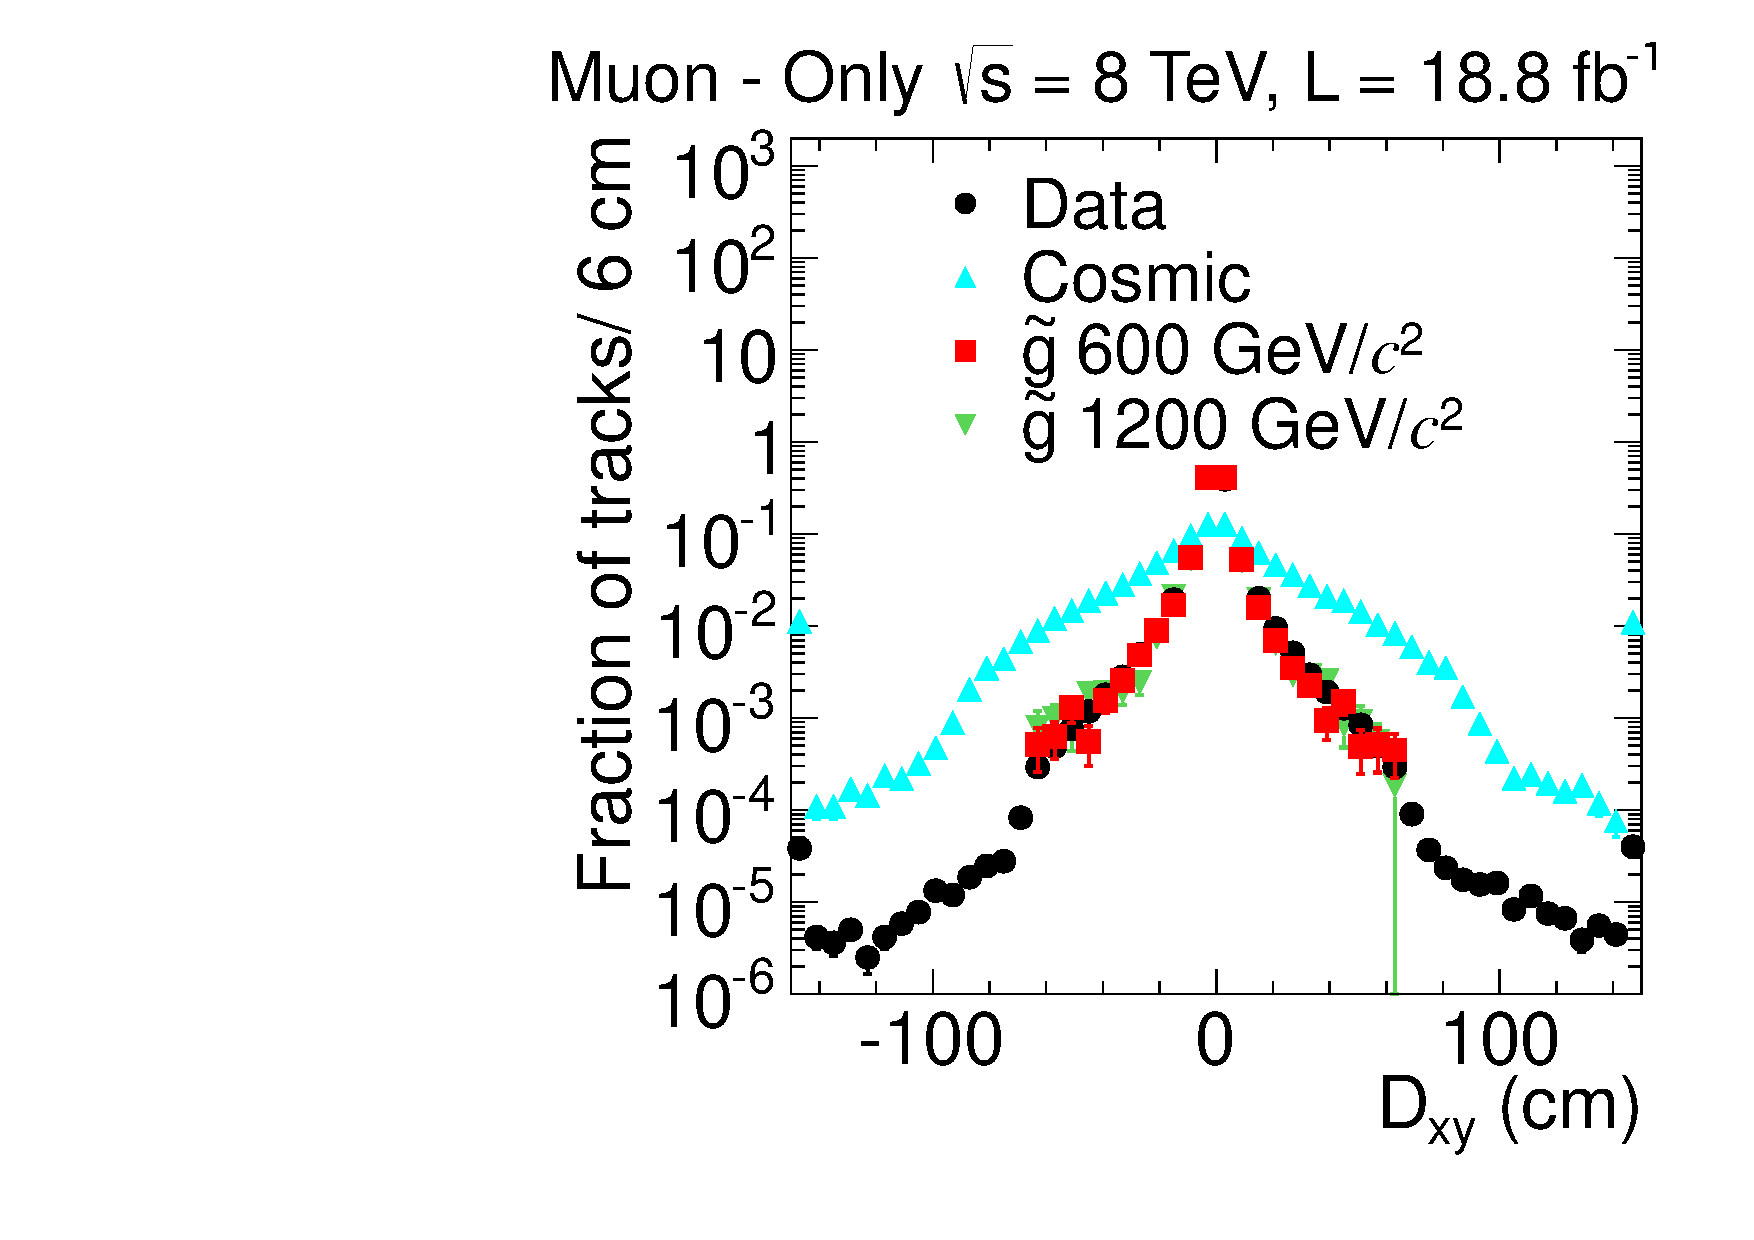
\includegraphics[clip=false, trim=0.0cm 0cm 0.0cm 0cm, width=0.48\textwidth]{figures/muonly/Selection_Comp_8TeV_Cosmic_Dxy_BS}
  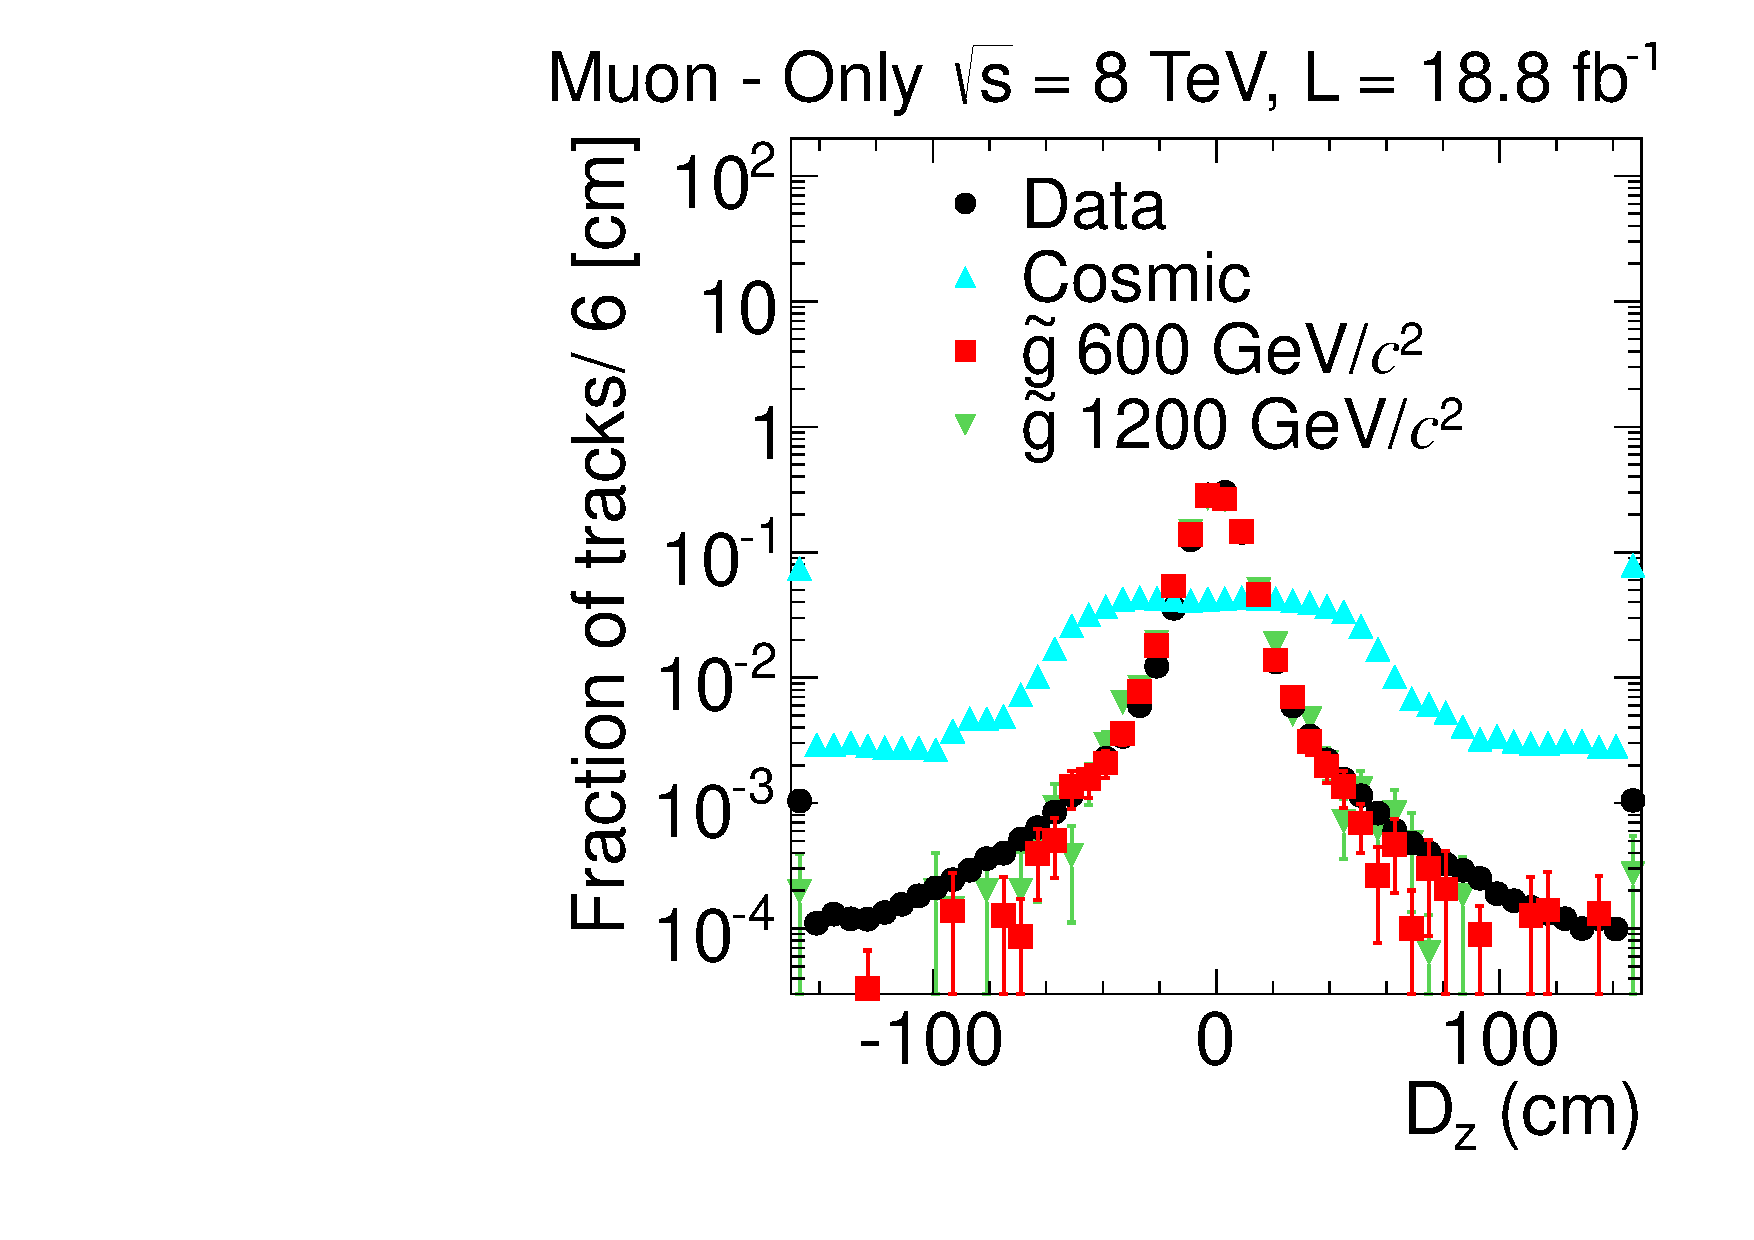
\includegraphics[clip=false, trim=0.0cm 0cm 0.0cm 0cm, width=0.48\textwidth]{figures/muonly/Selection_Comp_8TeV_Cosmic_Dz_BS} \\
  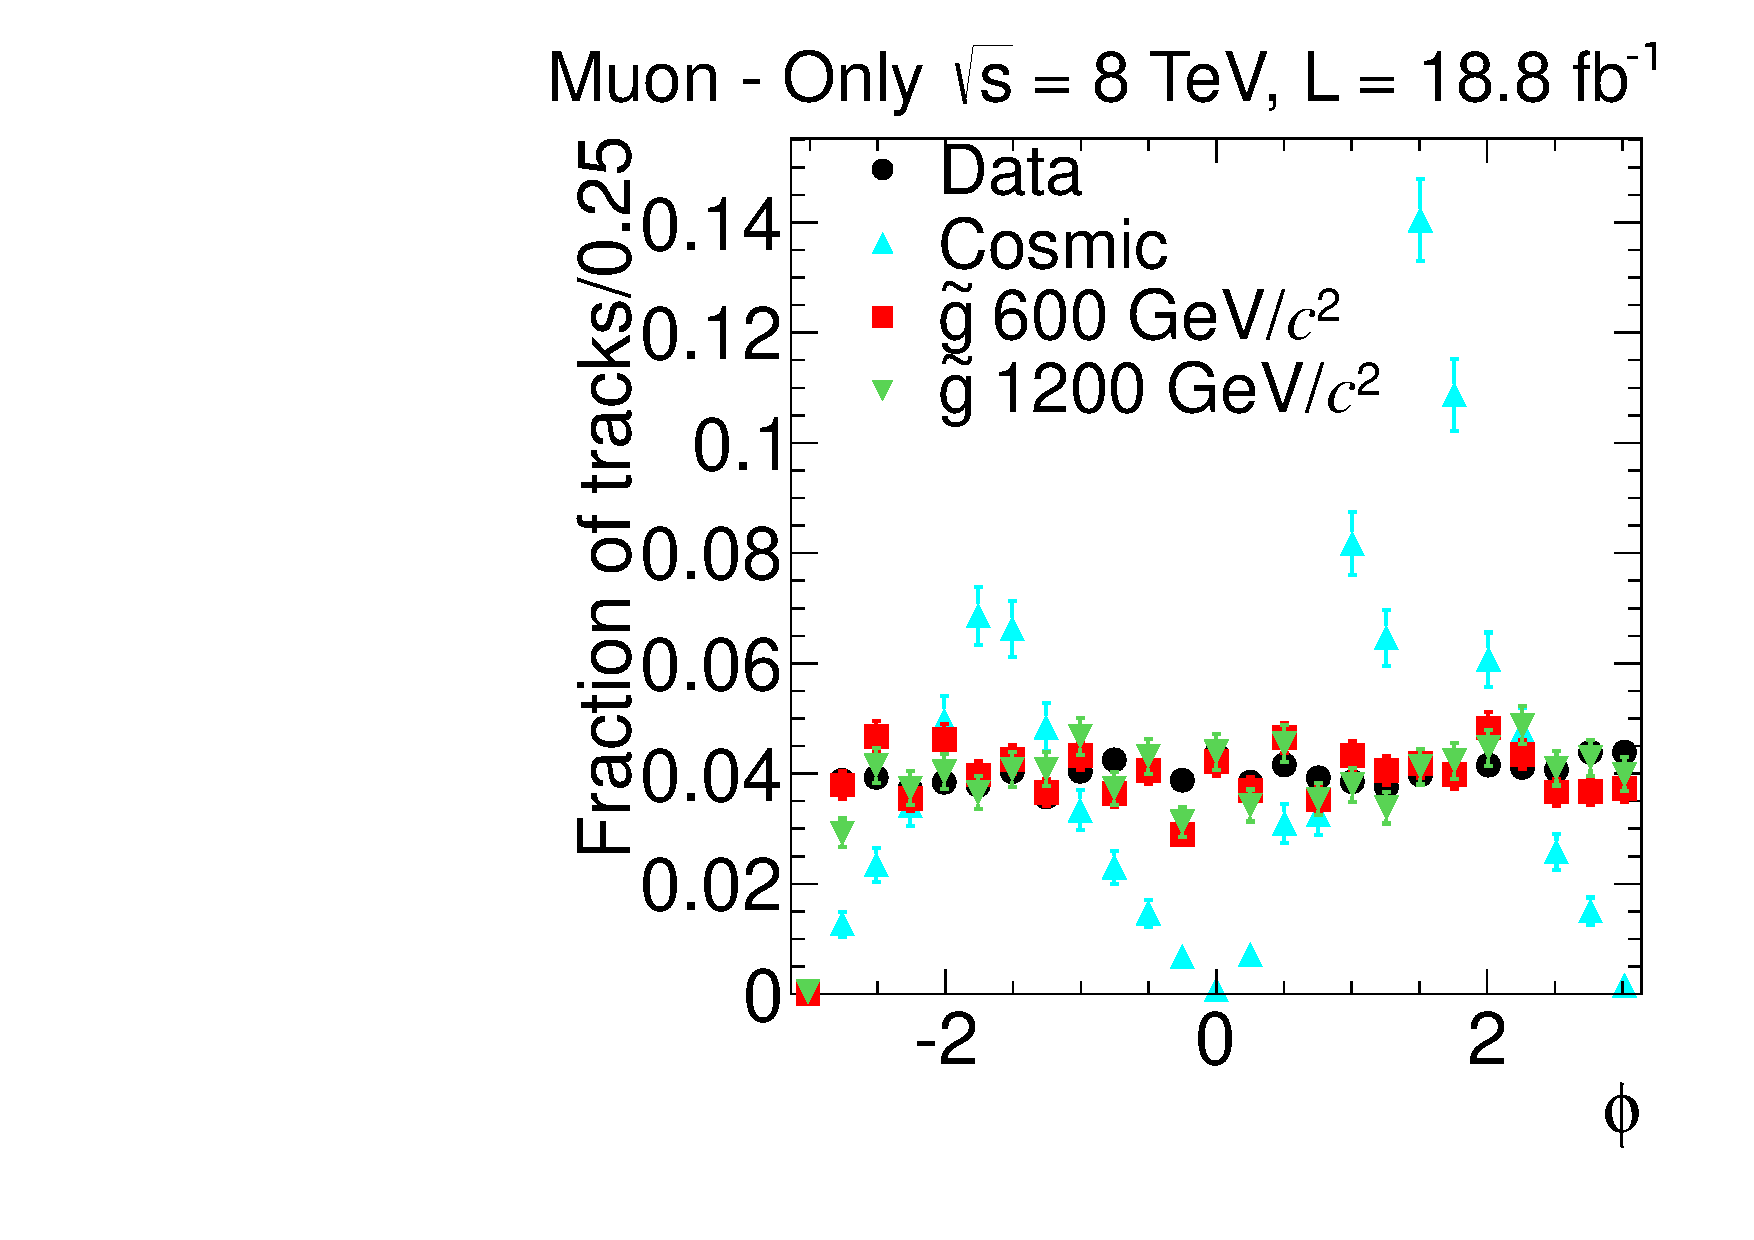
\includegraphics[clip=false, trim=0.0cm 0cm 0.0cm 0cm, width=0.48\textwidth]{figures/muonly/Selection_Comp_8TeV_Cosmic_Phi_BS}
  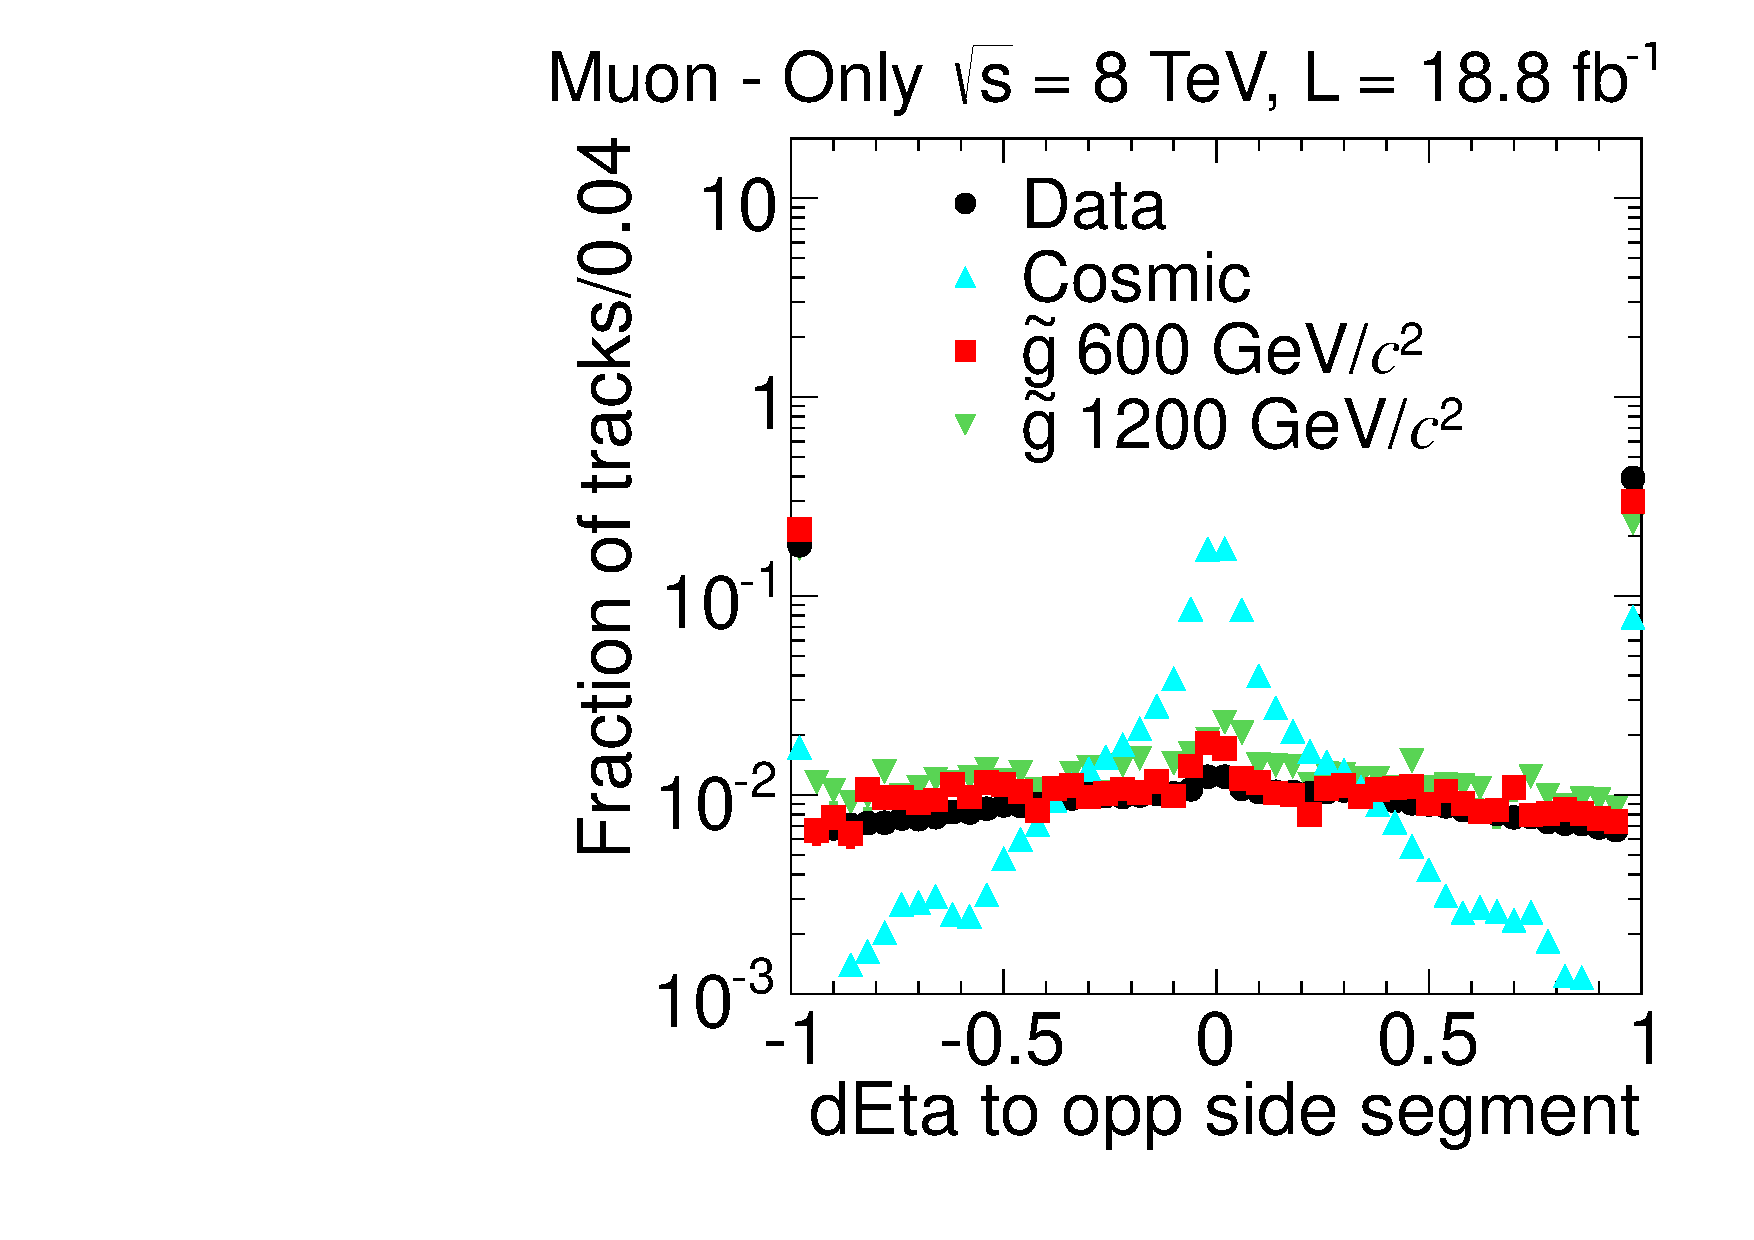
\includegraphics[clip=false, trim=0.0cm 0cm 0.0cm 0cm, width=0.48\textwidth]{figures/muonly/Selection_Comp_8TeV_Cosmic_SegMinEtaSep_BS}
  \caption[Distribution of transverse and longitudinal displacement, $\phi$, and $\eta$ separation to muon segments
in the \muononly\ analysis for data, cosmic-ray muon control sample, and signal MC samples.]
{Distribution of various preselection variables in the \muononly\ analysis for data, cosmic-ray muon control sample, and signal MC samples.
Top row: Distribution of transverse (left) and longitudinal displacement (right).
Bottom row: Distribution of the $\phi$ of the track (left) and the $\eta$ separation of the track to muon segments (right). The rightmost bin in the
$\eta$ separation plot includes tracks where no segments were found.}
    \label{fig:MuOnlyPreselC}
\end{figure}

\subsection{Preselection for \tktof\ \label{sec:tktofpreselection}}

The \tktof\ analysis applies cuts on the inner tracker track, which has a much better $p_T$ and impact parameter resolution than the muon system track.
The track is required to have $p_T > 45$~GeV and  $|\eta| < 2.1$ to match the trigger level requirements. 
Quality cuts are applied as low quality background tracks can have mismeasured momentum and potentially high fluctuations in \dedx.
The inner track is required to have at least eight hits in the inner tracker with at least two coming from the pixel detector. At least 80\% of the hits associated with the track
must be considered valid. As in~\cite{Chatrchyan:2012sp}, a cleaning procedure is applied to the hits before calculating \dedx\ that is 
intended to remove anomalous energy loss from overlapping tracks, nuclear interactions, and hard $\delta$-rays.
There must be at least six measurements passing this cleaning.
Figure~\ref{fig:TkMuPreselA} shows these variables for data and signal MC samples.

\begin{figure}
\centering
  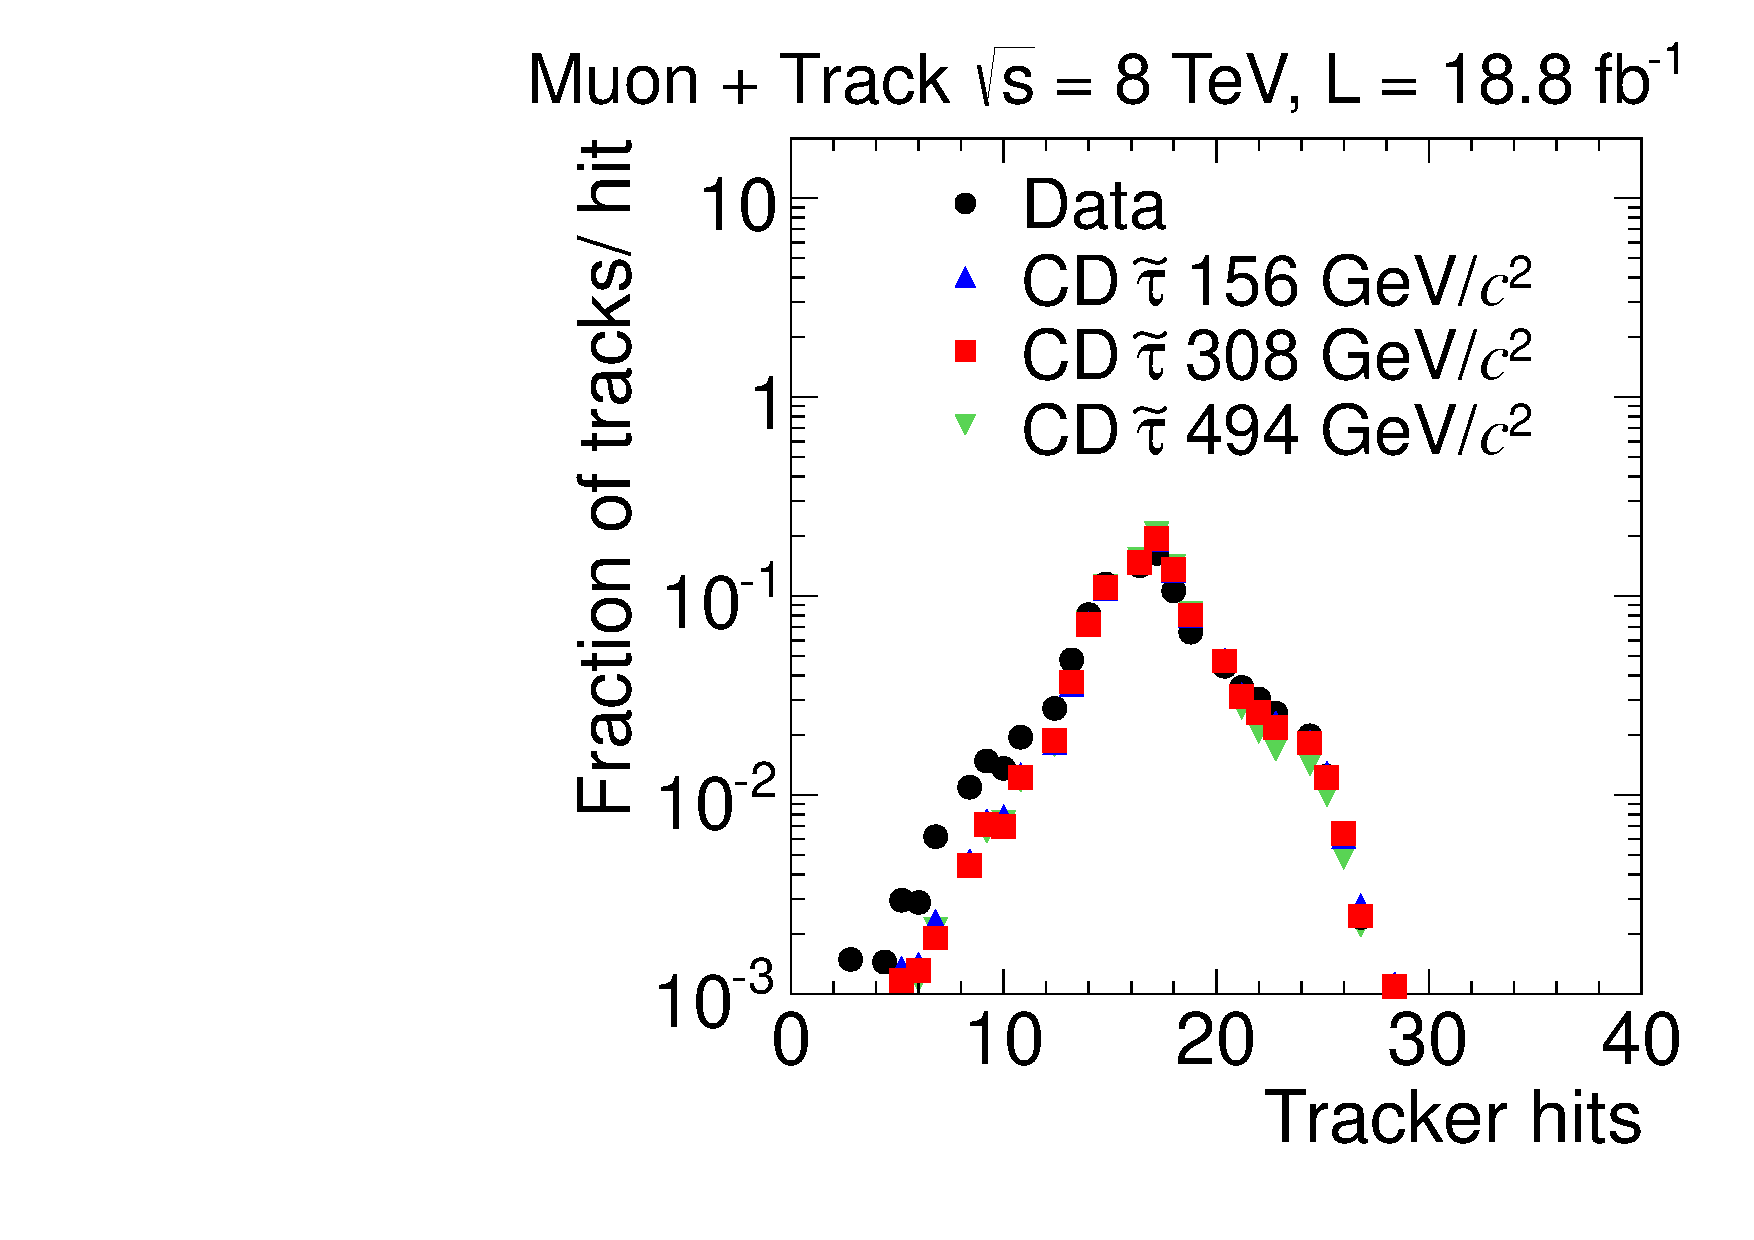
\includegraphics[clip=false, trim=0.0cm 0cm 0.0cm 0cm, width=0.48\textwidth]{figures/tkmu/Selection_Comp_8TeV_GMStau_NOH_BS}
  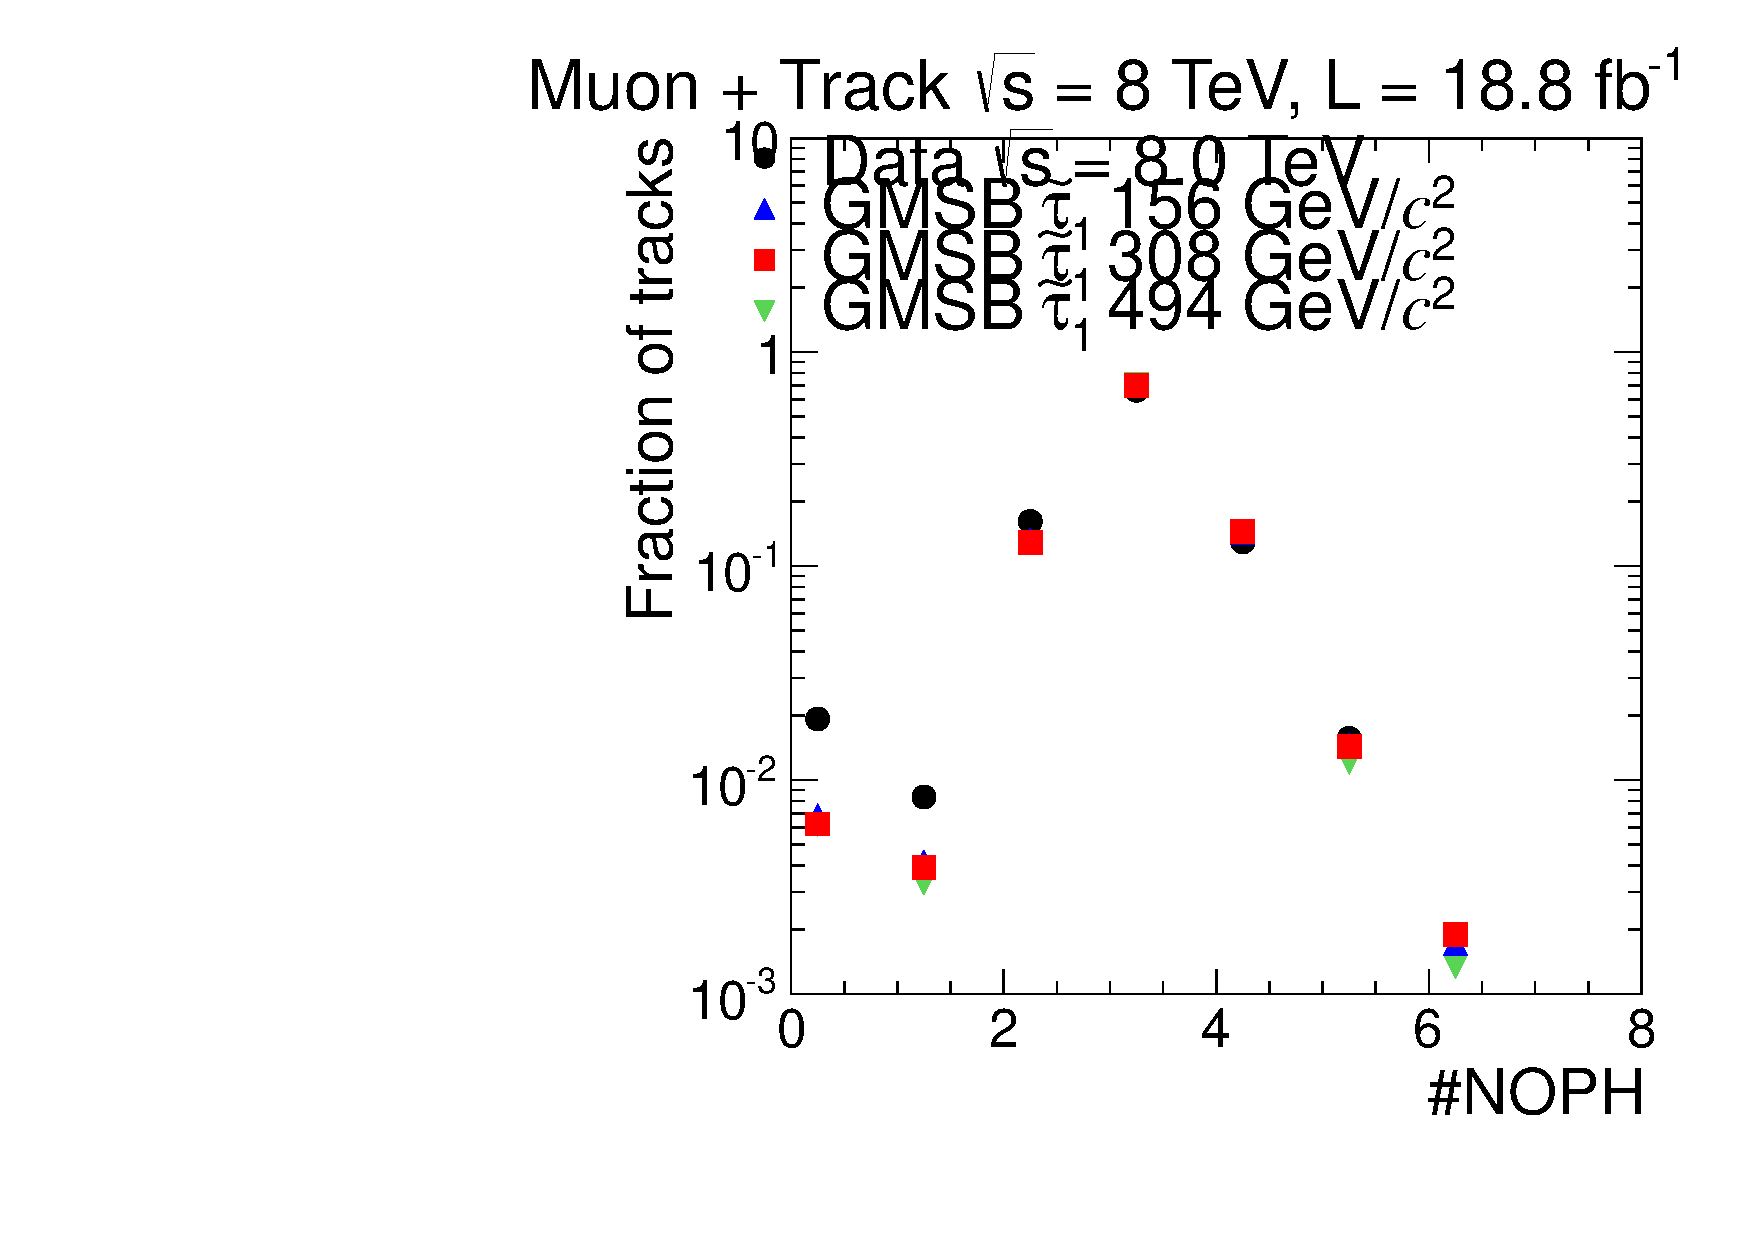
\includegraphics[clip=false, trim=0.0cm 0cm 0.0cm 0cm, width=0.48\textwidth]{figures/tkmu/Selection_Comp_8TeV_GMStau_NOPH_BS} \\
  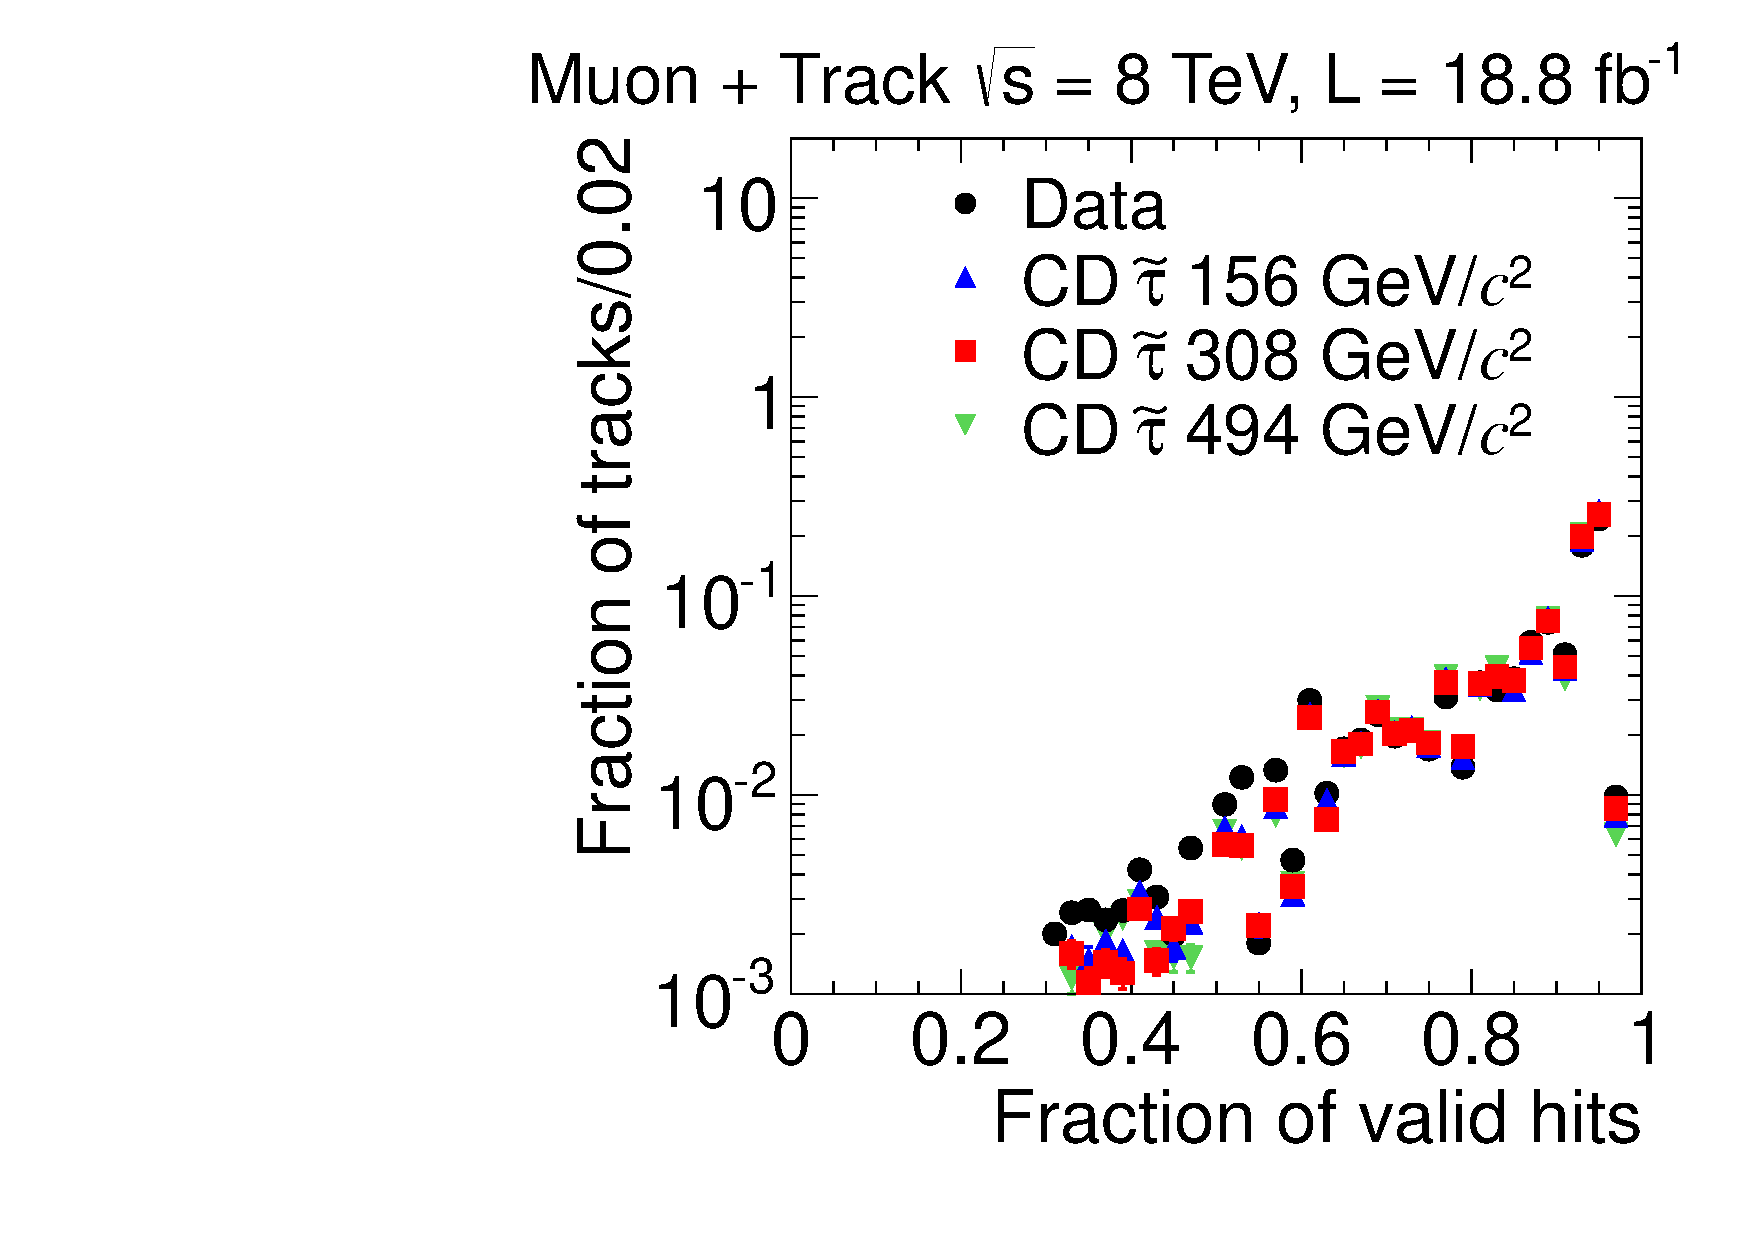
\includegraphics[clip=false, trim=0.0cm 0cm 0.0cm 0cm, width=0.48\textwidth]{figures/tkmu/Selection_Comp_8TeV_GMStau_NOHFraction_BS}
  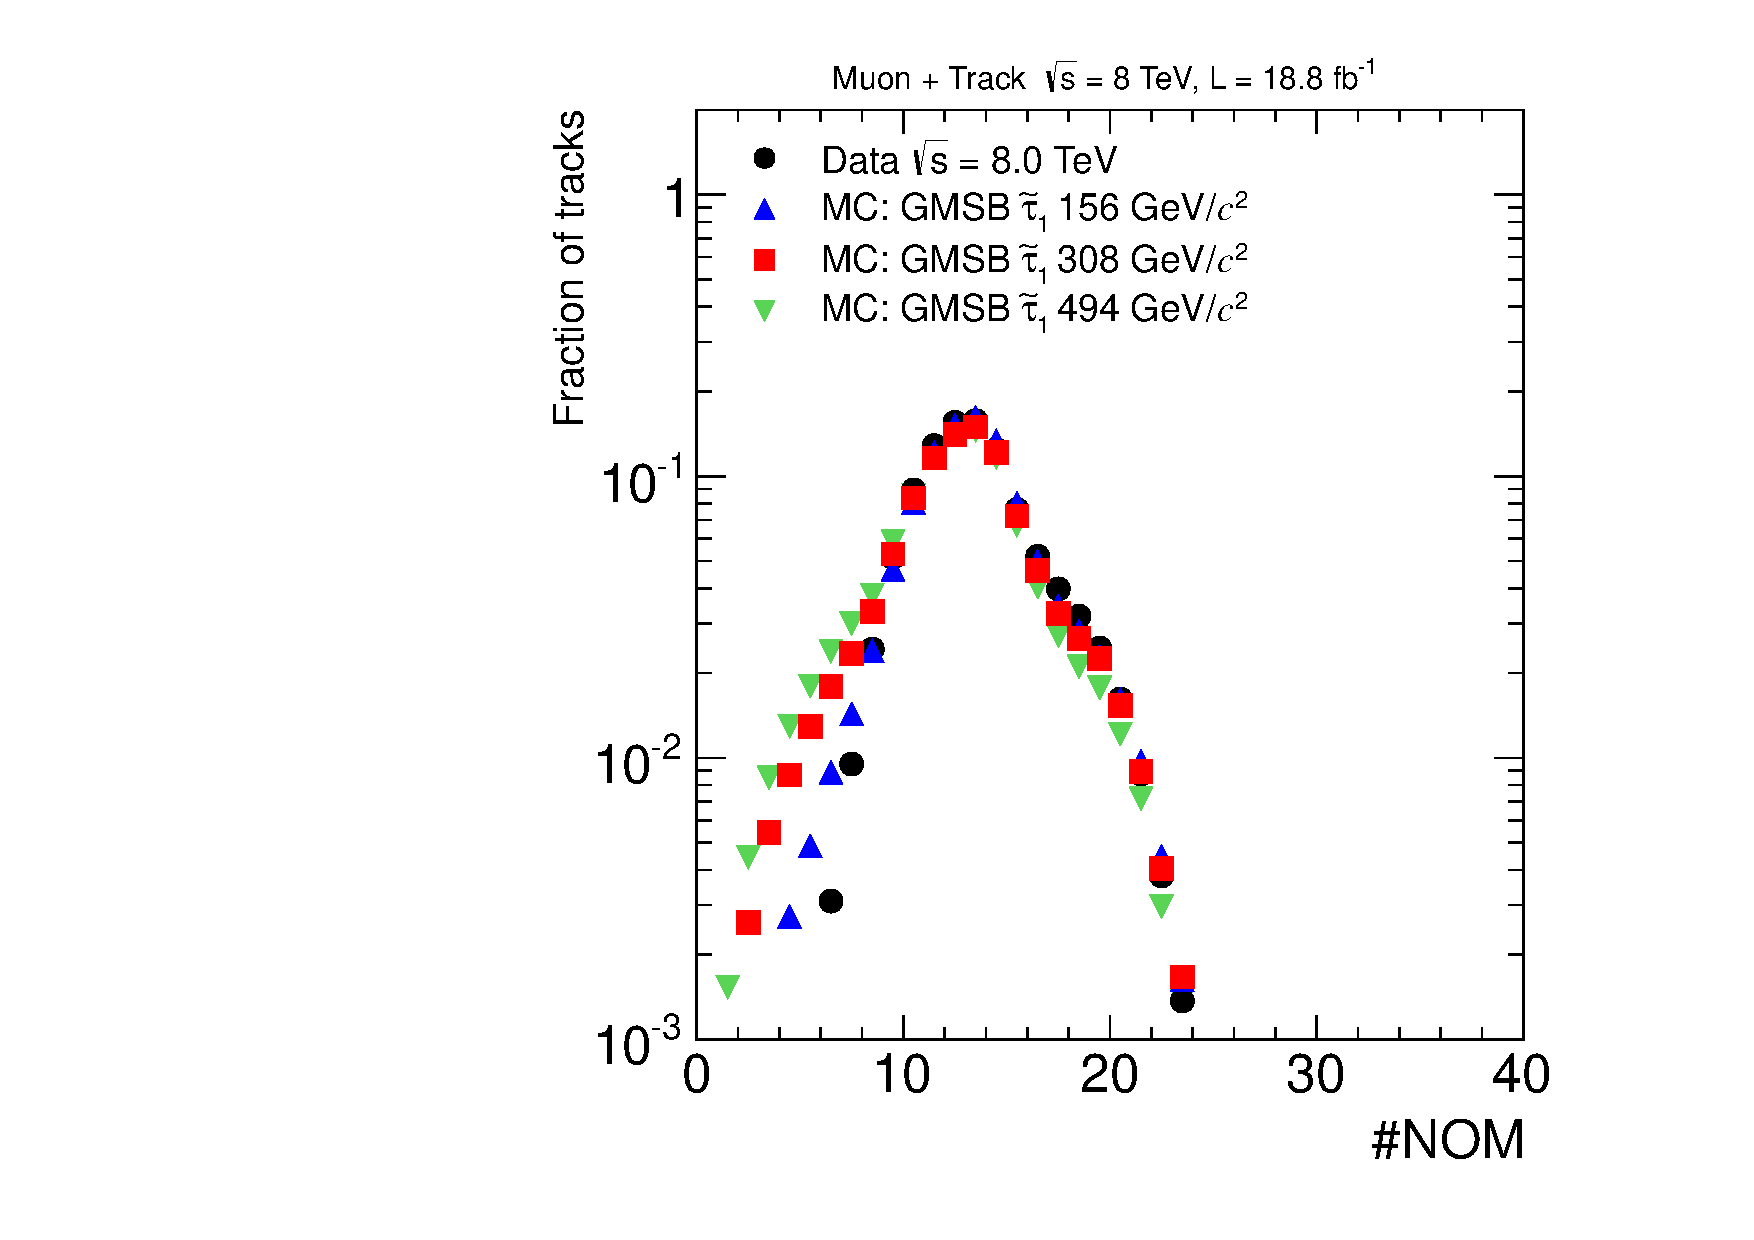
\includegraphics[clip=false, trim=0.0cm 0cm 0.0cm 0cm, width=0.48\textwidth]{figures/tkmu/Selection_Comp_8TeV_GMStau_NOM_BS}
  \caption[Distribution of number of tracker and pixel hits, fraction of valid tracker hits, and number of \dedx\ measurements in the \tktof\ analysis for data and signal MC samples.]
{Distribution of various preselection variables in the \tktof\ analysis for data and signal MC samples.
Top row: Number of tracker (left) and pixel (right) hits.
Bottom row: Fraction of valid tracker hits (left) and number of measurements used for the \dedx\ calculation (right).}
    \label{fig:TkMuPreselA}
\end{figure}

The relative uncertainty on the track $p_T$ ($\sigma_{p_T}/p_T$) must be less than 0.25 and the $\chi^2$ per degree of freedom must be less than five.
While cosmic-ray muons are expected to be a negligible background in the \tktof\ analysis, loose cuts are placed on the impact parameter of the track;
these cuts are nearly 100\% efficient for signal particles.
The displacement of the track with respect to the primary vertex
with the smallest longitudinal displacement must be less than 0.5~cm in both the transverse and longitudinal directions.
Figure~\ref{fig:TkMuPreselB} shows the $p_T$ uncertainty, $\chi^2$ per degree of freedom, and $d_z$ and $d_{xy}$ displacement for data and signal MC samples.

\begin{figure}
\centering
  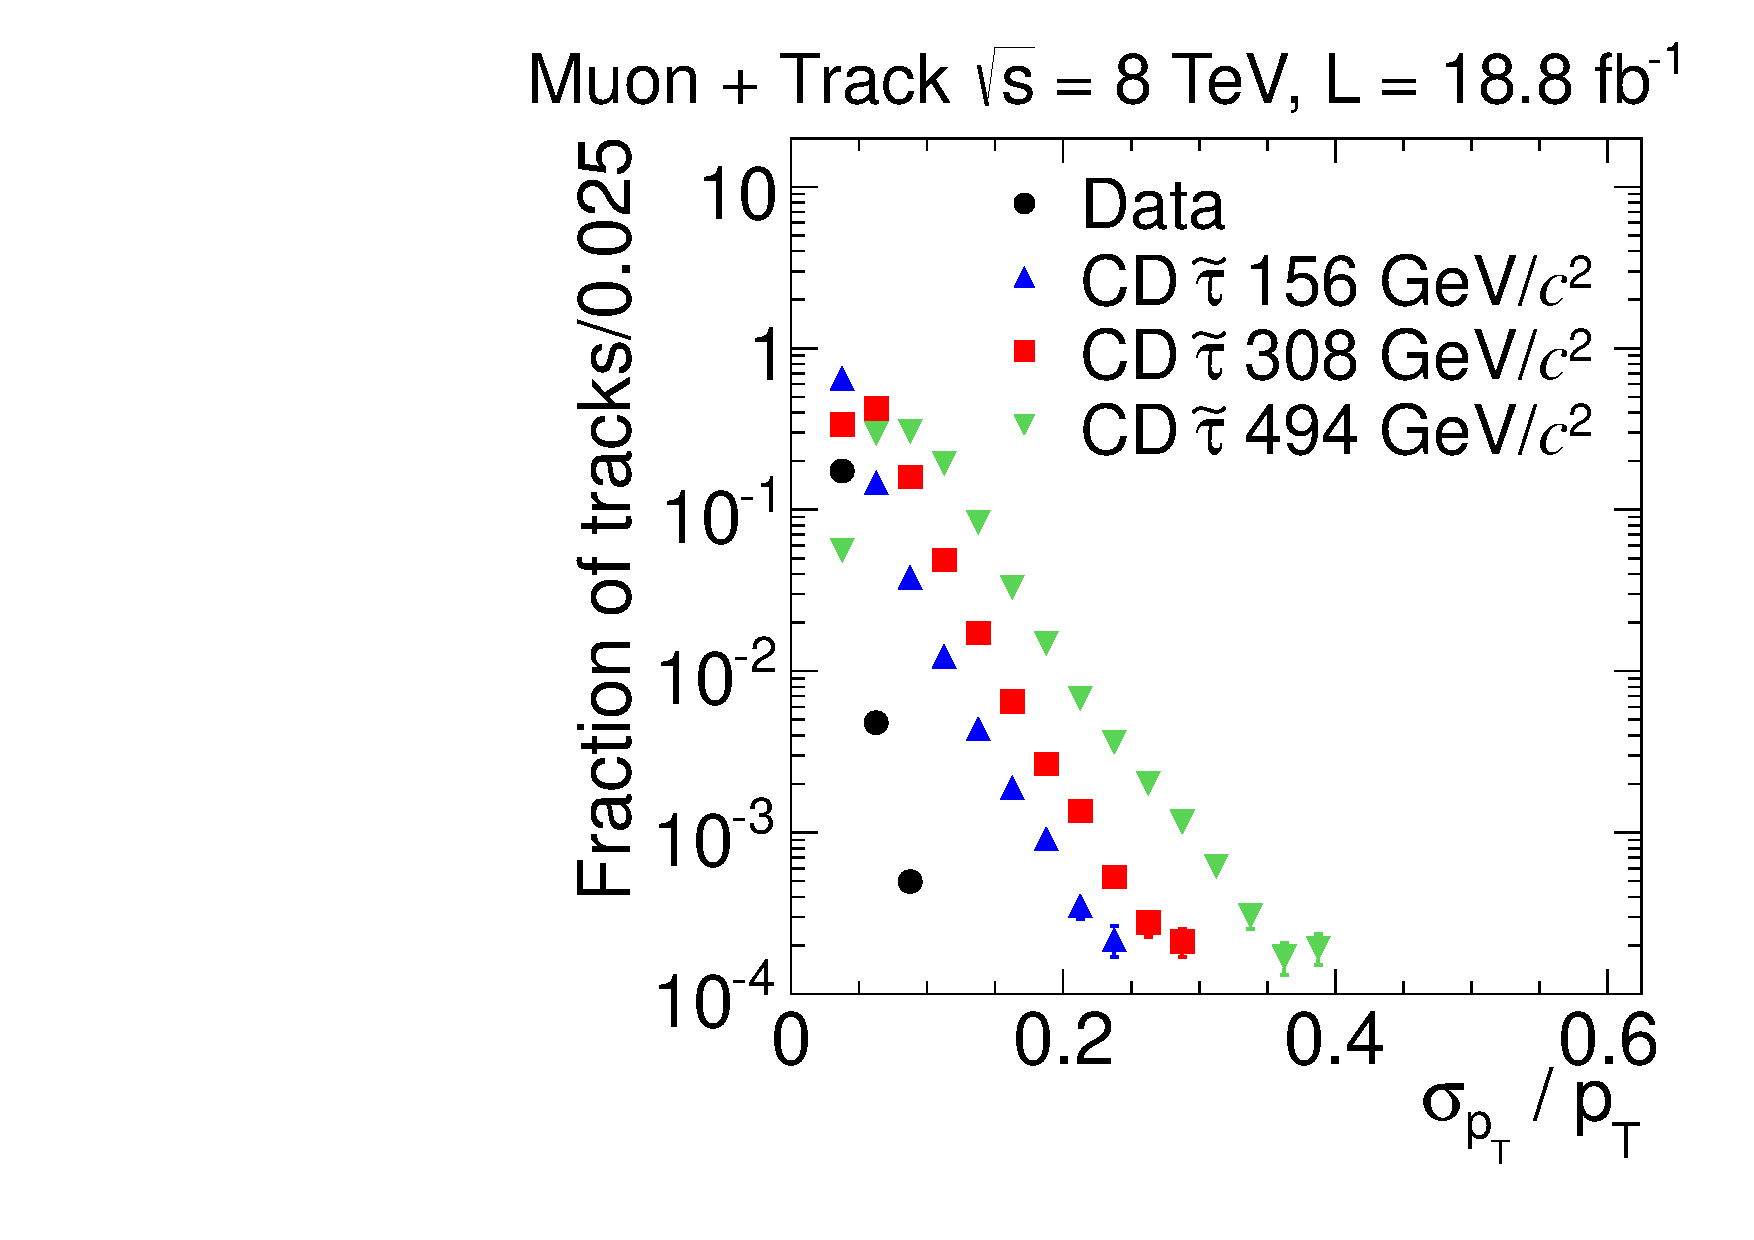
\includegraphics[clip=false, trim=0.0cm 0cm 0.0cm 0cm, width=0.48\textwidth]{figures/tkmu/Selection_Comp_8TeV_GMStau_Pterr_BS}
  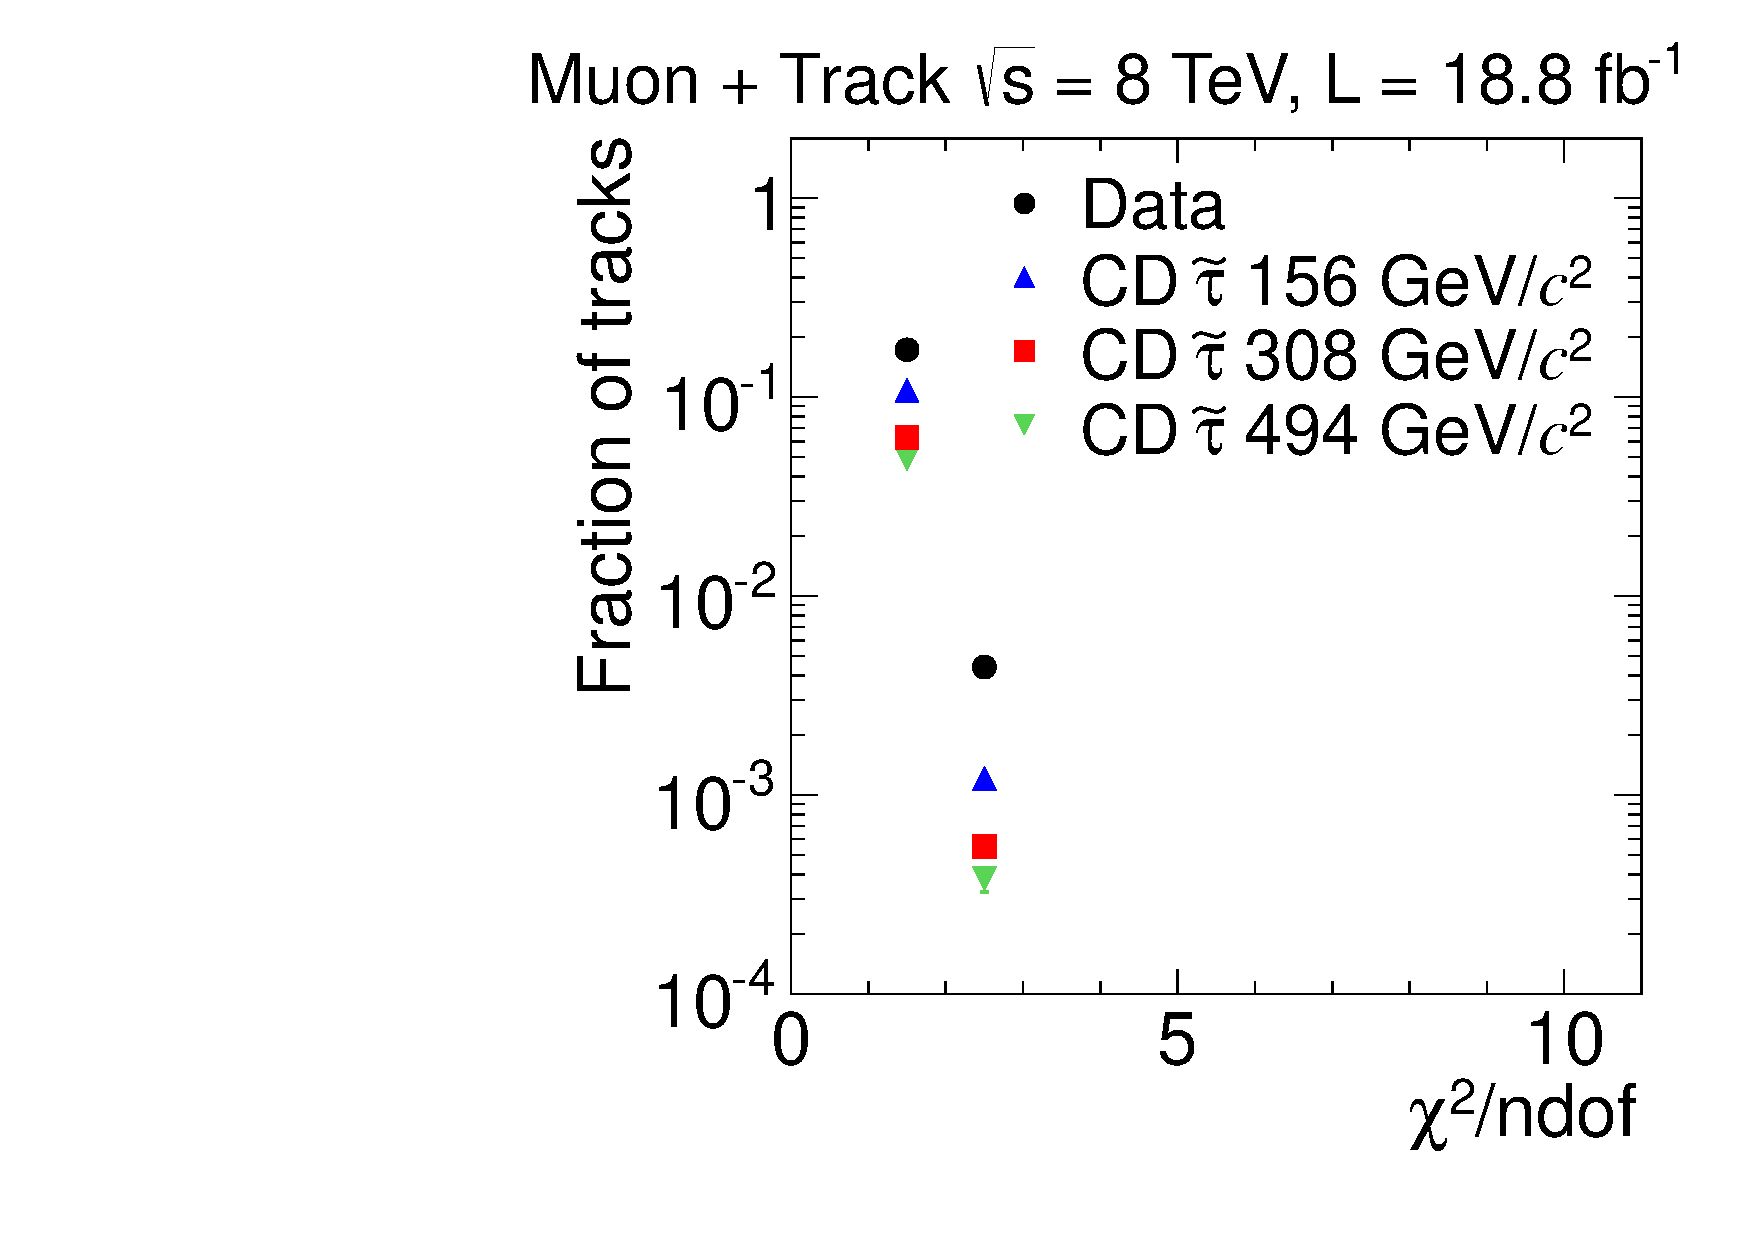
\includegraphics[clip=false, trim=0.0cm 0cm 0.0cm 0cm, width=0.48\textwidth]{figures/tkmu/Selection_Comp_8TeV_GMStau_Chi2_BS} \\
  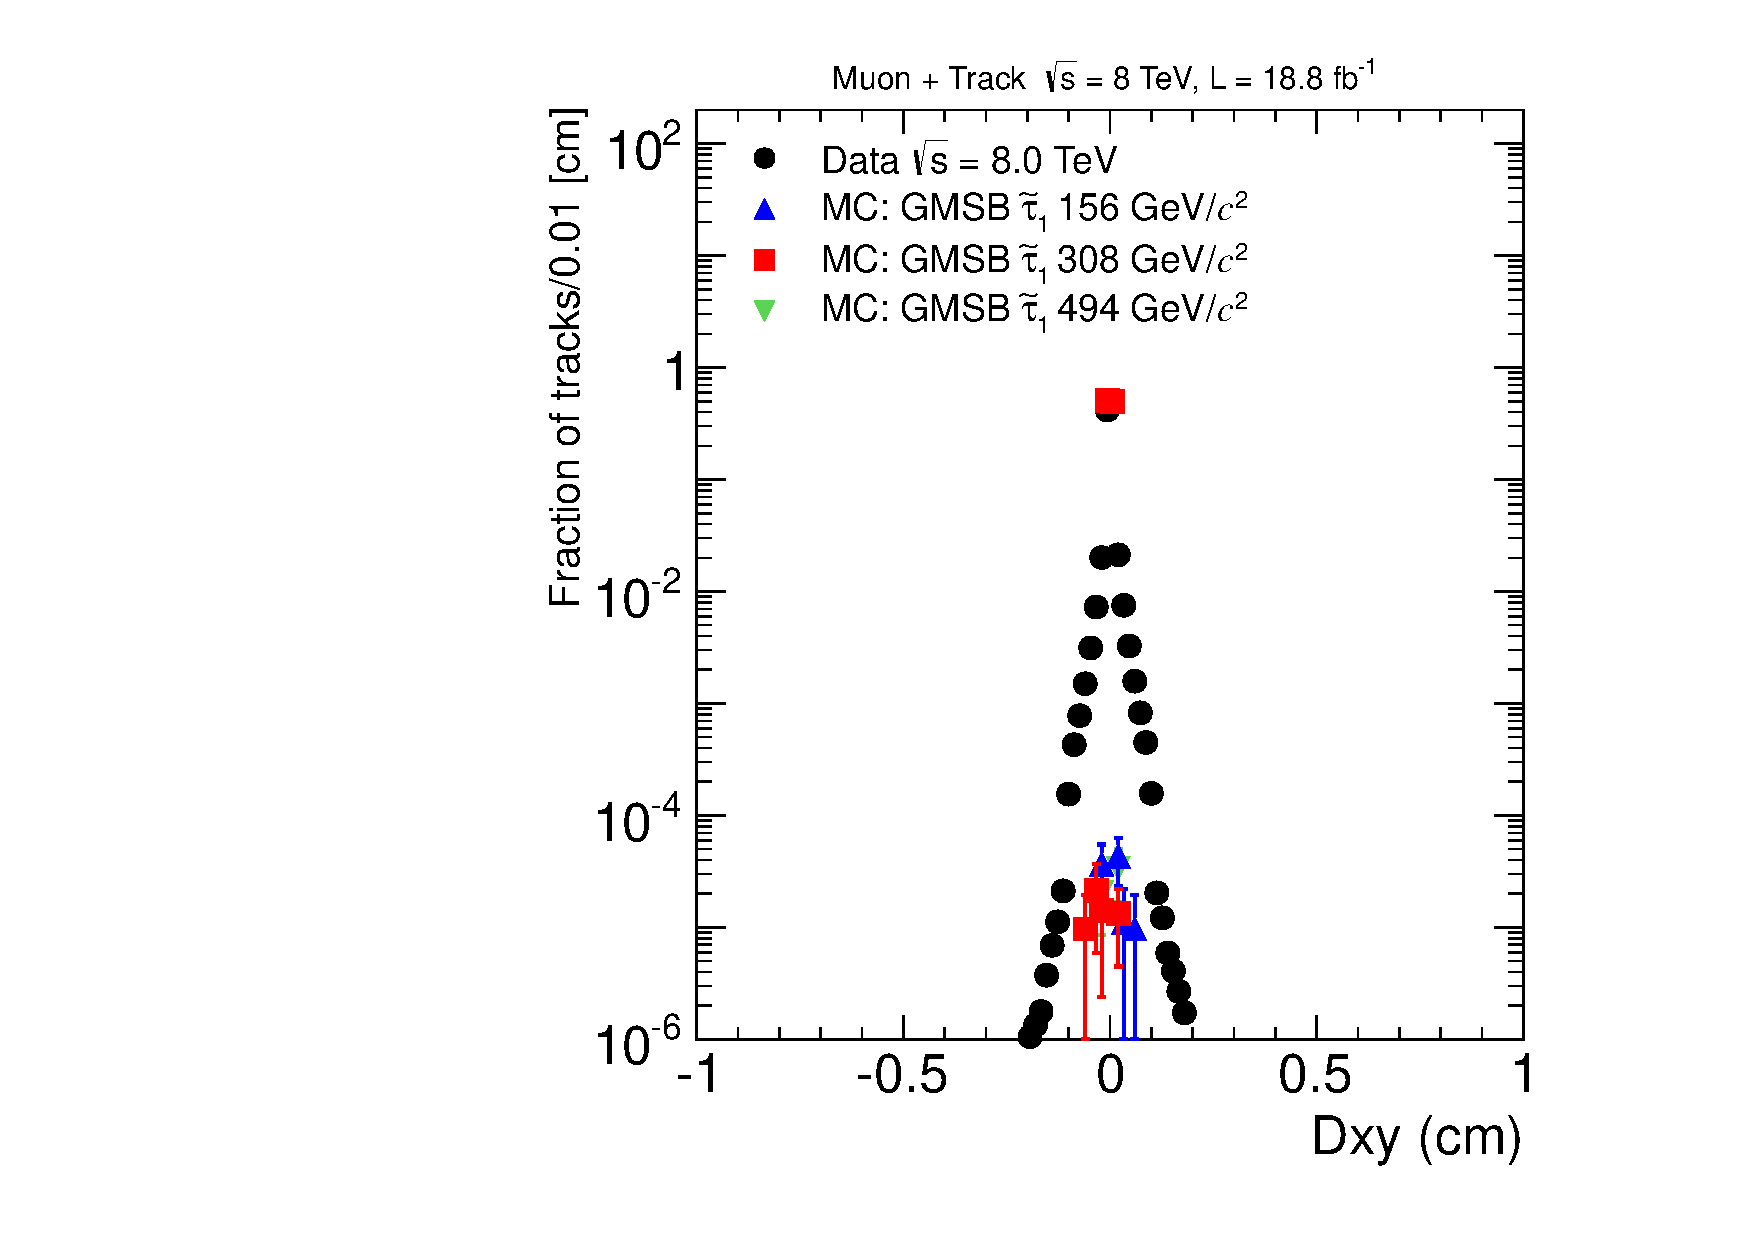
\includegraphics[clip=false, trim=0.0cm 0cm 0.0cm 0cm, width=0.48\textwidth]{figures/tkmu/Selection_Comp_8TeV_GMStau_Dxy_BS}
  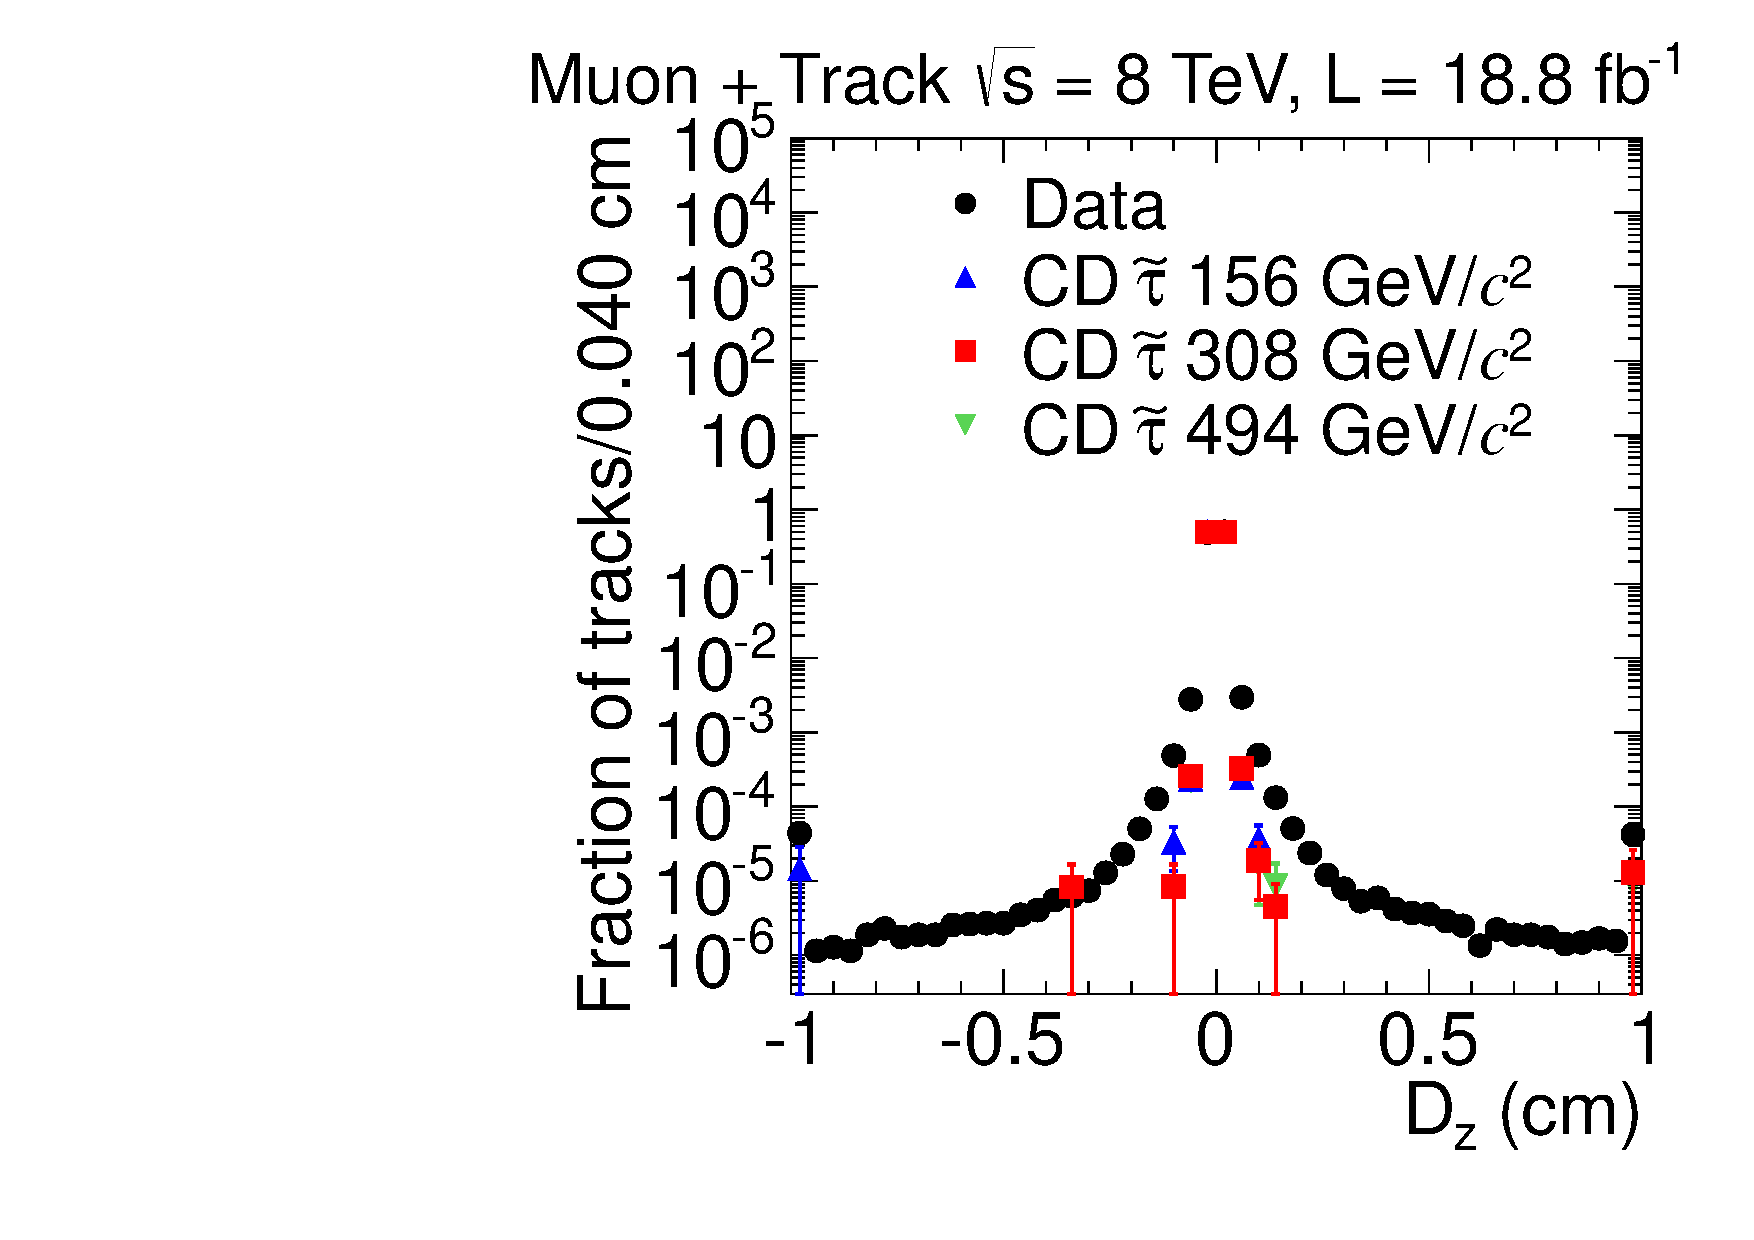
\includegraphics[clip=false, trim=0.0cm 0cm 0.0cm 0cm, width=0.48\textwidth]{figures/tkmu/Selection_Comp_8TeV_GMStau_Dz_BS}
  \caption[Distribution of relative \pt\ uncertainty, $\chi^2$ per degree of freedom, and transverse and longitudinal
displacement in the \tktof\ analysis for data and signal MC samples.]
{Distribution of various preselection variables in the \tktof\ analysis for data and signal MC samples.
Top row: Relative $p_T$ uncertainty (left) and $\chi^2$ per degree of freedom (right).
Bottom row: Displacement in the transverse (left) and longitudinal (right) directions.}
    \label{fig:TkMuPreselB}
\end{figure}

Isolation cuts are also applied in the \tktof\ analysis. Isolated means that there not be high energy particles near the track.
This is required to reduce the background from jets where overlapping tracks could give
anomalously high \dedx\ values. The isolation cuts are kept very loose as the goal is not to find isolated particles but just to reject very high energy jets.
Specifically, the sum of the momentum of the tracks within 0.3 in $\eta-\phi$ 
space of the track (excluding the track itself) is required to be less than 50 GeV. Additionally, the total
amount of energy measured in the calorimeter within a radius of 0.3 in $\eta-\phi$ space to the track divided by the track momentum must be less than 0.3.

Additionally, the \tktof\ analysis uses the same cuts on the \invbeta\ uncertainty and number of measurements as the \muononly\ analysis.
Figure~\ref{fig:TkMuPreselC} shows the isolation and \invbeta\ variables for data and signal MC samples.

\begin{figure}
\centering
  \includegraphics[clip=false, trim=0.0cm 0cm 0.0cm 0cm, width=0.48\textwidth]{figures/tkmu/Selection_Comp_8TeV_GMStau_IsolT_BS}
  \includegraphics[clip=false, trim=0.0cm 0cm 0.0cm 0cm, width=0.48\textwidth]{figures/tkmu/Selection_Comp_8TeV_GMStau_IsolE_BS} \\
  \includegraphics[clip=false, trim=0.0cm 0cm 0.0cm 0cm, width=0.48\textwidth]{figures/tkmu/Selection_Comp_8TeV_GMStau_TOFError_BS}
  \includegraphics[clip=false, trim=0.0cm 0cm 0.0cm 0cm, width=0.48\textwidth]{figures/tkmu/Selection_Comp_8TeV_GMStau_nDof_BS}
  \caption[Distribution of tracker and calorimeter isolation as well as the \invbeta\ measurement number of degrees of freedom and uncertainty
in the \tktof\ analysis for data and signal MC samples.]
{Distribution of various preselection variables in the \tktof\ analysis for data and signal MC samples.
Top row: Sum momentum of tracks within 0.3 (left) and calorimeter energy within 0.3 divided by track momentum (right).
Bottom row: Distribution of the \invbeta\ measurement uncertainty (left) and the number of degrees of freedom (right).}
    \label{fig:TkMuPreselC}
\end{figure}

\subsection{Preselection for \tkonly\ and \multi\ \label{sec:otherpreselection}}

The \tkonly\ analysis applies the same preselection as the \tktof\ analysis except the cuts on the timing measurement are not applied, as the tracks
are not required to be reconstructed in the muon system. 
%The \fract\ analysis uses preselection like \tkonly\ but inverting the \ih\ requirement
%to be less than 2.8 and requiring no tracks with \pt\ greater than 45 GeV to have an opening angle with the track greater than 2.8 radians.

The \multi\ analysis applies
the same selection criteria as the \tktof\ analysis except the cut on relative isolation less than 0.3 and the cleaning of the hits used for the \dedx\ calculation
is not done. The cleaning procedure is not applied because the amount of charge deposited is proportional to $Q^2$ meaning that even a $Q=2e$ HSCP will
deposit four times as much charge as a $Q=1e$ HSCP. As the tracker saturates for a energy loss approximately three times that expected for a MIP, many of the hits from $Q>1e$ HSCP
will be saturated; this can confuse the cleaning procedure. Additionally, as the high charge samples deposit so much charge, 
there will still be good signal/background separation even with longer tails in the \dedx\ distribution.
Figure~\ref{fig:Multi} shows the number of measurements passing the cleaning for multiply charged samples.
% and the opening angle described above for fractionally charged samples.

\begin{figure}
\centering
%  \includegraphics[clip=false, trim=0.0cm 0cm 0.0cm 0cm, width=0.48\textwidth]{figures/fract/Selection_Comp_8TeV_DY_OpenAngle_BS}
  \includegraphics[clip=false, trim=0.0cm 0cm 0.0cm 0cm, width=0.48\textwidth]{figures/multi/Selection_Comp_8TeV_DY_QG_NOM_BS}
  \caption{Distribution of number of \dedx\ measurements passing cleaning for samples of three different charges
    \label{fig:Multi}}
\end{figure}

\subsection{Summary of Preselection \label{sec:summarypreselection}}

The preselection criteria applied on the track in the muon system used in the \muononly, \tktof, and \multi\ analyses are summarized in Table~\ref{tab:preselectionSA}.
The preselection criteria applied on the track in the inner tracker used in the \tktof, \tkonly, and \multi\ analyses are summarized in Table~\ref{tab:preselectionTk}.

%\begin{table}
% \begin{center}
%  \caption{Preselection criteria used in the various analyses}
%     \label{tab:preselection}
%  \begin{tabular}{|l|c|c|c|c|} \hline
%                                            & Muon               & Muon+ & {\em multiple}            & Track       \\
%                                            & Only               & track & {\em charge}              & Only        \\ \hline
%   Track Type                               & Muon               & \multicolumn{2}{c|}{Inner + muon} & Inner       \\ \hline
%   $|\eta|$                                 & \multicolumn{4}{c|}{$< 2.1$}                                         \\ \hline
%   $p_T$ (GeV)                              & $> 80$             & \multicolumn{3}{c|}{$> 45$}                     \\ \hline
%   $d_z$ and $d_{xy}$ (cm)                  & $< 15$             & \multicolumn{3}{c|}{$< 0.5$}                    \\ \hline
%   \# DT or CSC Stations                    & $> 1$              & \multicolumn{3}{c|}{/}                          \\ \hline
%   Opp. segment $|\eta|$ difference         & $> 0.1$            & \multicolumn{3}{c|}{/}                          \\ \hline
%   $|\phi|$                                 & $< 1.2$ OR $> 1.9$ & \multicolumn{3}{c|}{/}                          \\ \hline
%   $|\delta t|$ to other beam crossing (ns) & $> 5$              & \multicolumn{3}{c|}{/}                          \\ \hline
%   \# TOF Measurements                      & \multicolumn{3}{c|}{$> 7$}                             & /           \\ \hline
%   $\sigma_{1/\beta}$                       & \multicolumn{3}{c|}{$< 0.07$}                          & /           \\ \hline
%   $1/\beta$                                & \multicolumn{3}{c|}{$> 1$}                             & /           \\ \hline
%   $\sigma_{p_T}/p_T$                       & /                  & \multicolumn{3}{c|}{$< 0.25$}                   \\ \hline
%   Track $\chi^2/d.o.f$                     & /                  & \multicolumn{3}{c|}{$< 5$}                      \\ \hline
%   \# Pixel Hits                            & /                  & \multicolumn{3}{c|}{$> 1$}                      \\ \hline
%   \# Tracker Hits                          & /                  & \multicolumn{3}{c|}{$> 7$}                      \\ \hline
%   Frac. Valid Hits                         & /                  & \multicolumn{3}{c|}{$> 0.8$}                    \\ \hline
%   \# \dedx\ Measurements                   & /                  & \multicolumn{3}{c|}{$> 5$}                      \\ \hline
%   \ih\ (MeV/cm)                            & /                  & \multicolumn{3}{c|}{ $> 3.0$}                   \\ \hline
%   \dedx\ Strip Shape Test                  & /                  & yes     & no                        & yes       \\ \hline
%   $\Sigma p_T^{trk} (\Delta R < 0.3)$ (GeV)& /                  & \multicolumn{3}{c|}{$< 50$}                     \\ \hline
%   $E_{cal}(\Delta R < 0.3)/p$              & /                  & $< 0.3$ & /                         & $< 0.3$   \\ \hline
%  \end{tabular}
% \end{center}
%\end{table}

\begin{table}
 \begin{center}
  \caption{Summary of preselection criteria on muon system qualities used in the various analyses as defined in the text.
     \label{tab:preselectionSA}}
  \begin{tabular}{|l|c|c|c|} \hline
                                            & \muononly\ & \tktof\  &  $|Q|>1e$    \\ \hline
   \# TOF measurements                      & \multicolumn{3}{c|}{$> 7$}   \\ \hline
   $\sigma_{1/\beta}$                       & \multicolumn{3}{c|}{$< 0.07$}\\ \hline
   $1/\beta$                                & \multicolumn{3}{c|}{$> 1$}   \\ \hline
   $|\eta|$                                 & $< 2.1$              & \multicolumn{2}{c|}{$-$} \\ \hline
   $p_T$ ($GeV/c$)                            & $> 80$      & \multicolumn{2}{c|}{$-$} \\ \hline
   $d_z$ and $d_{xy}$ (cm)                  & $< 15$      & \multicolumn{2}{c|}{$-$} \\ \hline
   \# DT or CSC stations                         & $> 1$      & \multicolumn{2}{c|}{$-$} \\ \hline
   Opp. segment $|\eta|$ difference              & $> 0.1$    & \multicolumn{2}{c|}{$-$} \\ \hline
   $|\phi|$                                      & $< 1.2$ OR $> 1.9$    & \multicolumn{2}{c|}{$-$} \\ \hline
   $|\delta t|$ to other beam crossing (ns)      & $>5$    & \multicolumn{2}{c|}{$-$} \\ \hline
  \end{tabular}
 \end{center}
\end{table}

\begin{table}
 \begin{center}
  \caption{Summary of preselection criteria on the silicon tracker qualities used in the various analyses as defined in the text.
     \label{tab:preselectionTk}}
  \begin{tabular}{|l|c|c|c|} \hline
                                            & \tktof\ & \tkonly\  &  $|Q|>1e$    \\ \hline
   $|\eta|$                                 & \multicolumn{3}{c|}{$< 2.1$}                            \\ \hline
   $p_T$ ($GeV/c$)                            & \multicolumn{3}{c|}{$> 45$}               \\ \hline
   $d_z$ and $d_{xy}$ (cm)                  & \multicolumn{3}{c|}{$< 0.5$}              \\ \hline
   $\sigma_{p_T}/p_T$                       & \multicolumn{3}{c|}{$< 0.25$}             \\ \hline
   Track $\chi^2/{n_d}$           & \multicolumn{3}{c|}{$< 5$}                    \\ \hline
   \# Pixel hits                            & \multicolumn{3}{c|}{$> 1$}                \\ \hline
   \# Tracker hits                          & \multicolumn{3}{c|}{$> 7$}                \\ \hline
   Frac. Valid hits                         & \multicolumn{3}{c|}{$> 0.8$}              \\ \hline
   $\Sigma p_{T}^{trk} (\Delta R < 0.3)$ ($GeV/c$) & \multicolumn{3}{c|}{$< 50$}             \\ \hline
   \# \dedx\ measurements                   & \multicolumn{3}{c|}{$> 5$}                \\ \hline
   \dedx\ strip shape test                  & \multicolumn{2}{c|}{yes}       & no       \\ \hline
   $E_{cal}(\Delta R < 0.3)/p$              & \multicolumn{2}{c|}{$< 0.3$}   & $-$      \\ \hline
  \end{tabular}
 \end{center}
\end{table}

The total preselection efficiency is shown in Tables~\ref{tab:preselectionEff} and ~\ref{tab:preselectionEffA} for the SUSY and modified DY samples, respectively.
The efficiencies are presented with respect to HSCP reconstructed as a track in CMS.
The inefficiency for the \muononly\ analysis mostly arises from the cuts used to suppress the background from cosmic-ray muons.
The other analyses lose efficiency due to quality requirements on the inner track and \dedx\ measurement
which are necessary to constrain the background from misreconstructed tracks.
Additionally, as CMS reconstruction generally assumes signatures of SM particles, HSCP tracks can have a lower quality than a SM particle would.
The requirements are set trying to balance keeping the signal efficiency high while maintaining a low background contamination of the signal region.


\begin{table}
 \begin{center}
  \caption[Preselection efficiency for a few benchmark SUSY samples in the \muononly, \tktof, and \tkonly\ analyses]
{Preselection efficiency for a few benchmark SUSY samples in each analysis.  
This efficiency is with respect to the reconstructed HSCP track (i.e. muon system track for the \muononly\ analysis and muon system plus inner tracker 
for the \tktof\ analysis).
The fraction of glueballs assumed for the gluino samples is given in parentheses at the end of the signal name.}
     \label{tab:preselectionEff}
   \begin{tabular}{|l|c|c|c|} \hline
Model         & \muononly\        & \tktof\        & \tkonly\  \\ \hline
%         & muon-           & track        & track  \\
%Model                    & only           & +muon        & only   \\ \hline
%Gluino 500    & \multirow{2}{*}{44\%} & \multirow{2}{*}{-}    & \multirow{2}{*}{-}  \\
%GeV (1.0)     &                         &                       &                  \\ \hline
%Guino 1000    & \multirow{2}{*}{40\%} & \multirow{2}{*}{-}    & \multirow{2}{*}{-} \\
%GeV (1.0)     &                         &                       &                  \\ \hline
%Gluino 500    & \multirow{2}{*}{44\%} & \multirow{2}{*}{60\%}    & \multirow{2}{*}{70\%} \\
%GeV (0.1)     &                         &                       &                     \\ \hline
%Gluino 1000   & \multirow{2}{*}{43\%} & \multirow{2}{*}{42\%} & \multirow{2}{*}{51\%} \\
%GeV (0.1)     &                         &                       &                     \\ \hline
%Gluino(CS)    & \multirow{2}{*}{-}    & \multirow{2}{*}{-}    & \multirow{2}{*}{64\%} \\
%5500 GeV (0.1) &                       &                       &                       \\ \hline
%Gluino(CS)    & \multirow{2}{*}{-}    & \multirow{2}{*}{-}    & \multirow{2}{*}{47\%} \\
%1000 GeV(0.1) &                         &                       &                     \\ \hline
%Stop 600      & \multirow{2}{*}{48\%} & \multirow{2}{*}{53\%} & \multirow{2}{*}{61\%} \\
%GeV           &                         &                       &                     \\ \hline
%Stop (CS)     & \multirow{2}{*}{56\%} & \multirow{2}{*}{-}    & \multirow{2}{*}{56\%} \\
%600 GeV       &                         &                       &                     \\ \hline
%CD Stau     & \multirow{2}{*}{-}    & \multirow{2}{*}{76\%}    & \multirow{2}{*}{78\%} \\
%370 GeV       &                         &                       &                     \\ \hline%


Gluino 500 GeV (1.0)   & 44\% & -    & -  \\
%GeV (1.0)     &     	      	      	&     	      	      	&     	      	   \\ \hline
Guino 1000 GeV (1.0)   & 40\% & -    & - \\ 
%GeV (1.0)     &     	      	      	&     	      	      	&     	      	   \\ \hline
Gluino 500 GeV (0.1)   & 44\% & 60\%    & 70\% \\
%GeV (0.1)     &     	      	      	&     	      	      	&     	      	      \\ \hline
Gluino 1000 GeV (0.1)  & 43\% & 42\% & 51\% \\
%GeV (0.1)     &     	      	      	&     	      	      	&     	      	      \\ \hline
Gluino(CS) 500 GeV (0.1)   & -    & -    & 64\% \\
%500 GeV (0.1) &                       &                       &                       \\ \hline
Gluino(CS) 1000 GeV (0.1)   & -    & -    & 47\% \\
%1000 GeV(0.1) &     	      	      	&     	      	      	&     	      	      \\ \hline
Stop 600 GeV     & 48\% & 53\% & 61\% \\
%GeV           &     	      	      	&     	      	      	&     	      	      \\ \hline
Stop (CS) GeV    & 56\% & -    & 56\% \\
%600 GeV       &     	      	      	&     	      	      	&     	      	      \\ \hline
CD Stau 370 GeV    & -    & 76\%    & 78\% \\
%370 GeV       &     	      	      	&     	      	      	&     	      	      \\ \hline
\hline
   \end{tabular}
 \end{center}
\end{table}


\begin{table}
 \begin{center}
  \caption
[Preselection efficiency for a few benchmark modified DY samples in the \tktof, \tkonly, and \multi\ analyses.]
{Preselection efficiency for a few benchmark modified DY samples in each analysis.
This efficiency is with respect to the reconstructed HSCP track (i.e. muon system plus inner track for the \multi\ analysis and inner track for the \tkonly\ analysis).}
     \label{tab:preselectionEffA}
   \begin{tabular}{|l|c|c|c|} \hline
%              & track        & track        & {\em multiple} \\
%Model         & +muon        & only         & {\em charge}          \\ \hline
%%DY Q2o3       & \multirow{2}{*}{15\%}    & \multirow{2}{*}{17\%} & \multirow{2}{*}{-} \\
%%400 GeV       &                          &                       &                    \\ \hline
%DY $Q = 1e$         & \multirow{2}{*}{72\%}    & \multirow{2}{*}{76\%} & \multirow{2}{*}{75\%} \\
%600 GeV       &                          &                       &                       \\ \hline
%DY $Q = 3e$         & \multirow{2}{*}{-}    & \multirow{2}{*}{-}    & \multirow{2}{*}{71\%} \\
%600 GeV       &                          &                       &                       \\ \hline
%DY $Q = 5e$         & \multirow{2}{*}{-}    & \multirow{2}{*}{-}    & \multirow{2}{*}{50\%} \\
%600 GeV       &                          &                       &                       \\ \hline
%DY $Q 7e$         & \multirow{2}{*}{-}       & \multirow{2}{*}{-}    & \multirow{2}{*}{37\%} \\
%600 GeV       &                          &                       &                       \\ \hline

Model     & \tktof\    & \tkonly\        & \multi\ \\ \hline
DY $Q = 1e$ 600 GeV        & 72\%    & 76\% & 75\% \\
DY $Q = 3e$ 600 GeV        & -    & -    & 71\% \\
DY $Q = 5e$ 600 GeV        & -    & -    & 50\% \\
DY $Q = 7e$ 600 GeV        & -       & -    & 37\% \\
\hline
   \end{tabular}
 \end{center}
\end{table}


The distributions of $p_T$ and \invbeta\ for the \muononly\ analysis for data, cosmic-ray muon control sample, and various signal models is 
shown in Figure~\ref{fig:MuOnlySelVar} after applying the preselection requirements. Figure~\ref{fig:TkMuSelVar} shows the $p_T$, \invbeta, and \dedx\
distributions after applying the \tktof\ preselection cuts for data and various signal models.

\begin{figure}
\centering
  \includegraphics[clip=false, trim=0.0cm 0cm 0.0cm 0cm, width=0.48\textwidth]{figures/muonly/Selection_Comp_8TeV_Cosmic_Pt_BS}
  \includegraphics[clip=false, trim=0.0cm 0cm 0.0cm 0cm, width=0.48\textwidth]{figures/muonly/Selection_Comp_8TeV_Cosmic_TOF_BS} \\
  \caption[Distribution of \invbeta\ and \pt\ in the \muononly\ analysis for data, cosmic-ray muon control sample, and signal MC samples]
{Distribution of selection variables for data, cosmic-ray muon control sample, and signal MC samples.
Left: Distribution of $p_T$. Right: Distribution of \invbeta.}
    \label{fig:MuOnlySelVar}
\end{figure}

\begin{figure}
\centering
  \includegraphics[clip=false, trim=0.0cm 0cm 0.0cm 0cm, width=0.48\textwidth]{figures/tkmu/Selection_Comp_8TeV_GMStau_Pt_BS}
  \includegraphics[clip=false, trim=0.0cm 0cm 0.0cm 0cm, width=0.48\textwidth]{figures/tkmu/Selection_Comp_8TeV_GMStau_TOF_BS} \\
  \includegraphics[clip=false, trim=0.0cm 0cm 0.0cm 0cm, width=0.48\textwidth]{figures/tkmu/Selection_Comp_8TeV_GMStau_Is_BS}
  \includegraphics[clip=false, trim=0.0cm 0cm 0.0cm 0cm, width=0.48\textwidth]{figures/tkmu/Selection_Comp_8TeV_GMStau_Im_BS}
  \caption[Distribution of selection variables in the \tktof\ analysis for data and signal MC samples.]
{Distribution of section variables for data and signal MC samples.
Top row: Distribution of $p_T$ (left) and \invbeta\ (right).
Bottom row: Distribution of \ias\ (left) and \ih\ (right).}
    \label{fig:TkMuSelVar}
\end{figure}

\subsection{Tag and Probe Studies \label{sec:TagProbe}}
The study of the agreement between data and MC simulation for numerous muon qualities is done by the Muon POG of CMS.
The group provides scale factors for correcting MC samples to match data.
For all of the analyses except for \muononly\  it is sufficient to use results obtained from this group as the muon qualities
those analyses use are common within CMS.
However, as the \muononly\ analysis uses numerous variables which are unique to it, the results from the muon POG are not applicable to it.

For this reason, additional studies were performed to test the agreement of MC simulation with data.
The efficiency of the selections was checked with a tag-and-probe technique~\cite{2012JInst...7P0002T} using muons from Z boson decays.
% Z bosons decay to a particle and its anti-particle with the invariant mass of the particle--anti-particle
%pair equal to the mass of the Z boson they were created from.
The tag-and-probe procedure proceeds by requiring one muon, the ``tag'' muon, be found with a stringent selection while the other muon, the ``probe'' muon,
is required to be found with only a loose selection using only the silicon tracker. The efficiency to pass the preselection in the \muononly\ analysis
can then be estimated as the fraction of of the probes that pass the preselection. The background from processes other than Z bosons is small and is subtracted by
a simultaneous fit to the tag-probe invariant mass distributions of signal and background around the Z boson mass.
The efficiency estimated in data is compared with that found in MC samples. Scale factors are used to correct the MC samples for any discrepancy observed between the efficiencies.
The MC sample used does not contain any production from background processes.

The tag muon is required to pass the tight selection (see Section.~\ref{sec:timingintro}) recommended by the Muon POG and to match to an object that triggered the read out of CMS. 
The last requirement assures that no bias is introduced in the efficiency measurement by the need for the event to have been read out.
Additionally, the tag must pass the requirements of a skim that was used to reduce the data size to a level
making processing reasonable. The skim requirements are at least three \dedx\ measurements and \ih\ $> 3.0$ or \ih\ $< 2.8$.

A set of probe candidates is defined as tracks reconstructed in the inner tracker with no requirement
of muon system activity. The probes are required to have $p_T > 40$ GeV, $|\eta| < 2.1$, and the opposite charge of the tag muon.
The invariant mass of the tag-probe pair is then required to be within 10 GeV of the mass of the Z boson, 91 GeV.
The invariant mass distribution of the tag-probe pairs is fit using the
sum of two Voigtians (the convolution of a Lorentzian and a Gaussian) to represent the signal and an exponential for the background.

%The fit is found to agree well with the data.
%Figures~\ref{fig:MuOnlyTagProbeFitData} and ~\ref{fig:MuOnlyTagProbeFitMC} show sample fits to data and MC, respectively.
%It can be seen that the fits match well.
%The efficiency is extracted from these fits using a procedure from the muon POG.

%\begin{figure}
% \begin{center}
%  \includegraphics[clip=true, trim=0.0cm 7.0cm 0.0cm 0.0cm, width=0.95\textwidth]{figures/muonly/FitCanvasDataPtBin0}
% \end{center}
% \caption[Example fits to invariant mass distributions
%in the tag-and-probe procedure for the \muononly\ analysis for data.]
%{Example fits to invariant mass distributions
%in the tag-and-probe procedure for the \muononly\ analysis for data.
%Top left: Mass distribution and fit for probes passing the preselection. Top right: Mass distribution and fit for probes failing the preselection.
%Bottom left: Mass distribution and fit for all probes. Bottom right: Parameters extracted from the fit.}
%    \label{fig:MuOnlyTagProbeFitData}
%\end{figure}

%\begin{figure}
% \begin{center}
%  \includegraphics[width=0.95\textwidth]{figures/muonly/FitCanvasMCEtaBin6}
% \end{center}
% \caption[Example fits to invariant mass distributions
%in the tag-and-probe procedure for the \muononly\ analysis for MC.]
%{Same as Fig.~\ref{fig:MuOnlyTagProbeFitData} but for MC.}
%    \label{fig:MuOnlyTagProbeFitMC}
%\end{figure}

Figure~\ref{fig:MuOnlyTagProbeEff} shows the efficiency for the probes
to pass the preselection, except for the selection on $p_T$, against the probe
$p_T$, $\eta$, and the number of primary vertices in the event.
Overall the efficiency is approximately 75\% in data and 80\% in the MC sample.
The efficiency is mostly flat versus $p_T$ and number of vertices but does depend
on $\eta$.  The MC simulation is scaled by an $\eta$ dependent scale factor to correct for the discrepancy.

\begin{figure}
 \begin{center}
  \includegraphics[clip=false, trim=0.0cm 0cm 0cm 0cm, width=0.44\textwidth]{figures/muonly/pteff_Comp}
  \includegraphics[clip=false, trim=0.0cm 0cm 0cm 0cm, width=0.44\textwidth]{figures/muonly/etaeff_Comp}
  \includegraphics[clip=false, trim=0.0cm 0cm 0cm 0cm, width=0.44\textwidth]{figures/muonly/PVeff_Comp}
 \end{center}
 \caption[Efficiency to pass preselection cuts for the \muononly\ analysis as a function of \pt, $\eta$, and number of primary vertices]
{Efficiency to pass preselection cuts for the \muononly\ analysis.
Top row: As a function of $p_T$ (left) and $\eta$ (right)
Bottom row: As a function of number of primary vertices.}
   \label{fig:MuOnlyTagProbeEff}
\end{figure}

\section{Background Predictions \label{BackPred}}
All of the analyses count the number of tracks passing threshold values on some grouping of the $p_T$, \invbeta, 
and \ias\ variables. The \tktof\  and \tkonly\ analyses also place a requirement on the mass of the track as described below. There are two sources
of background considered in the analyses. 

The first is muons, or for the \tkonly\ analysis any charged SM particle, from the collisions in the LHC. Muons can pass the thresholds on the selection variables
for a variety of reasons.
All muons at the LHC will be traveling at very nearly the speed of light,
but finite detector resolution results in a smearing of the measured time of hits. This can cause muons to have a high measured \invbeta.
While muons in the momentum region of interest all deposit approximately
the same amount of energy in the tracker on average, the amount deposited in each interaction is subject to large variations. This can lead to muons
with a high \dedx\ value. Detector resolution can also contribute to muons with high \dedx.
Additionally, collision muons can have large reconstructed momentum, either due to true high momentum or detector mismeasurement
promoting a low momentum muon to a high reconstructed momentum. Detector mismeasurement is especially important for the momentum measured in the muon system.

Collision muons are predicted by exploiting the lack of correlation between the selection variables for muons through the $ABCD$ method.
In the $ABCD$ method, multiple bins are defined by whether the track passes thresholds on the selection variables. In the normal two dimensional version
of the $ABCD$ method, two selection variables are used and four regions are defined. The $A$ region has tracks failing both of the thresholds on the selection
variables, the $B$ ($C$) region fails only the threshold on the first (second) of the selection variables, and the $D$ region,
the signal region, passes the threshold on both selection
variables. The number of background muons in the $D$ region can be predicted as $B \times C / A$, where the letters represent the number of tracks in the regions.
This prediction holds as long as the probability for a background
muon to pass the threshold on one of the variables is independent of whether it passes the threshold of the other. Tests of the correlation between the selection variables are
given below.

The four different analyses use different combinations of the selection variables defined in Sec.~\ref{sec:SelVar}. 
With three different selection variables (\pt, \invbeta, \dedx), eight different bins are defined.
In order to simplify the nomenclature in this section, Table~\ref{tab:BinNames} 
defines the names of the bins (ranging from $A$-$H$) and whether they pass or fail the thresholds on the selection variables. For all
the selection variables passing means having a value above the threshold. If a selection variable
is not used in an analysis then it is taken to have passed. 

Only the \tktof\ analysis applies a threshold on all three selection variables and as such is the only one to use all eight bins.
An extended three-dimensional version of the $ABCD$ method is then used to make the prediction as is described in the \tktof\ subsection below.
The other three analyses use only the four bins where the unused variable is said to have passed. These analyses use the traditional two-dimensional $ABCD$ method
though the names of the bins may be different.
For all the analyses the D region is always the signal region. 

In order to perform systematic studies, the analyses that use \invbeta\ reverse the preselection requirement on \invbeta\ greater than one. This creates a group of tracks
measured as going faster than the speed of light, making it signal free. As the \invbeta\ distribution is close to symmetrical for background muons,
this region is very good for testing the background prediction. New bins are defined as in Table~\ref{tab:BinNames} but now \invbeta\ is said to have passed
if the value is below the threshold. The bins are referred to with a prime to denote that they are from the control region, so the new ``signal'' region would
be referred to as $D^{\prime}$.


\begin{table}
 \begin{center}
  \caption[Bin naming convention for background regions]
{Bin naming convention.  The signal region is always the D region.}
     \label{tab:BinNames}
  \begin{tabular}{|c|c|c|c|} \hline
   Name & $p_T$ & \invbeta\   & \dedx\  \\ \hline
   A    & Fail      & Fail            & Pass           \\ \hline
   B    & Fail      & Pass            & Pass           \\ \hline
   C    & Pass      & Fail            & Pass           \\ \hline
   D    & Pass      & Pass            & Pass           \\ \hline
   E    & Fail      & Fail            & Fail           \\ \hline
   F    & Fail      & Pass            & Fail           \\ \hline
   G    & Pass      & Fail            & Fail           \\ \hline
   H    & Pass      & Pass            & Fail           \\ \hline
  \end{tabular}
 \end{center}
\end{table}

The second source of background, important only for the \muononly\  analysis,
%and \fract\ analyses, 
is muons from cosmic-rays. 
As discussed in Section~\ref{sec:SM} muons from cosmic-rays
are constantly passing through CMS. Cosmic-ray muons will arrive to the muon system asynchronously with collisions in the LHC. Depending on exactly
when the cosmic-ray muon arrives in the muon system relative to collisions in the LHC this can give rise to a particle with a large \invbeta\ measurement.
The distribution of $p_T$ for cosmic-ray muons falls off at high momentum slower than for collision muons, as evidenced in Figure~\ref{fig:MuOnlySelVar} (left).
As cosmic-ray muons have different \invbeta and \pt\ distributions than collision muons they will not be accurately predicted with the same method used to predict
the collision-muon background in the \muononly\ analysis. A dedicated method using the cosmic-ray muon control sample is described below.

Cosmic-ray muons are not considered for the analyses that look for high-ionizing tracks as
out-of-time particles are not centered in the tracker's charge collection window.
This results in only a portion of their ionization energy loss being collected and their reconstructed \dedx\ being smaller than a collision muon.
Thus, cosmics have the signature of anomalously low reconstructed \dedx~\cite{CMS:2012xi} opposite of the signature for an HSCP.
%This combined with the impact parameter requirements applied at preselection makes cosmic-ray muons negligible for the analyses looking for high \dedx\ in the tracker.

For all the analyses, the expected background in the signal region is estimated by multiple different predictions.
The details on how the different predictions are found for each analysis are given in the corresponding subsection below.
The spread of the different background predictions can be used to estimate the systematic uncertainty for each analysis.

The following variables are defined:
\begin{equation}
\centering
\begin{split}
S^{syst+stat}_{N} &= \sqrt{\sum_i \left( x_i - \langle x \rangle  \right) ^2/(N-1)} \\
S^{stat}_{N} &= \sqrt{\sum_i \left( \sigma _i \right) ^2/N} \\
S^{syst} &= \sqrt{S_{syst+stat}^2-S_{stat}^2} \\
\end{split}
\label{eq:variance}
\end{equation}
where N is the number of background estimates made,
the sum is over N, $x_i$ is the value of the $i^{th}$ background estimate,
and $\sigma_i$ is the statistical uncertainty on
the $i^{th}$ background estimate. The first quantity is an estimator of the
standard deviation of the background estimates, which takes both statistical
and systematic contributions. The second quantity is adopted as an
estimator of the contribution of the statistical uncertainties
to the standard deviation. Finally, the last equation gives the systematic uncertainty on the background prediction assuming
the statistical and systematic uncertainties add in quadrature to give the standard deviation.

\subsection{Prediction for \muononly\ analysis \label{sec:MuOnlyPred}}

The collision muon  background in the \muononly\ analysis is predicted with the selection criteria of \invbeta\ and \pt\ in the $ABCD$  method.
%by exploiting the lack of correlation between the selection variables for background particles. 
The expected number of background tracks in the signal region $D$ (see Table~\ref{tab:BinNames}) is predicted as $B \times C / A$. 
%Tracks are divided into four groups based on whether they
%have $p_T$ and \invbeta\ values greater than the thresholds placed on these selection criteria. 
%The four groups are referred to as $A$,$B$,$C$, and $D$. The $A$ group contains tracks that have $p_T$ and \invbeta\ values lower than both selection thresholds
%while the $B$($C$) group contains tracks that have only the $p_T$ (\invbeta) below its threshold. The groups containing the tracks with \invbeta\
%below the its threshold only contains tracks with $1 < $\invbeta\ $< $ threshold. Tracks with \invbeta\ $< 1$ are used to evaluate how well the prediction performs.
%The $D$ group contains tracks passing both thresholds and is considered the signal region. 

%The predicted number of collision muons in the signal region is found via the relation $B \times C / A$. This relation is accurate so long as the ratio of tracks
%passing the \invbeta\ cut is the same regardless of whether the $p_T$ cut is passed, the statement is also true reversing the roles of \invbeta\ and $p_T$.
The $ABCD$ method only works if the probability to pass one of the thresholds is independent of the other variable.
However, it has been observed that a correlation exists between the $p_T$ and \invbeta\ measurements based on whether the track is in the barrel or forward
region of the detector as well as the number of DT or CSC stations containing valid hits. 
Six bins are created defined by the $\eta$ of the track, greater or less than 0.9; and the number of stations, 2, 3, or 4.
The distributions of \pt\ and \invbeta\ in the six regions is shown in Figure~\ref{fig:SelVarBinned}.
The predicted number of tracks in each bin is predicted separately and the total number of predicted background tracks is the sum of the six predictions.

\begin{figure}
\centering
  \includegraphics[clip=false, trim=0.0cm 0cm 0.0cm 0cm, width=0.48\textwidth]{figures/muonly/Selection_Data8TeV_Pt_Binned_BS}
  \includegraphics[clip=false, trim=0.0cm 0cm 0.0cm 0cm, width=0.48\textwidth]{figures/muonly/Selection_Data8TeV_TOF_Binned_BS}
\caption[Distribution of $p_T$ and \invbeta\ for data in different prediction regions in the \muononly\ analysis]
{Distribution of $p_T$ and \invbeta\ for data for six different regions depending on whether the track is in the barrel (Bar)
or forward (For) region of CMS and number of muon stations (Sta) used in the fit.}
    \label{fig:SelVarBinned}
\end{figure}

After the binning the correlation is small enough not to bias the background prediction as can be seen in Figs.~\ref{fig:MuOnlyControl} and~\ref{fig:MuOnlyControl4}.

\begin{figure}
\begin{center}
\includegraphics[clip=false, trim=0.0cm 0cm 0.0cm 0cm, width=0.48\textwidth]{figures/muonly/Control_Data8TeV_Pt_TOFSpectrum_Binned_0}
\includegraphics[clip=false, trim=0.0cm 0cm 0.0cm 0cm, width=0.48\textwidth]{figures/muonly/Control_Data8TeV_Pt_TOFSpectrum_Binned_3} \\
\includegraphics[clip=false, trim=0.0cm 0cm 0.0cm 0cm, width=0.48\textwidth]{figures/muonly/Control_Data8TeV_Pt_TOFSpectrum_Binned_1}
\includegraphics[clip=false, trim=0.0cm 0cm 0.0cm 0cm, width=0.48\textwidth]{figures/muonly/Control_Data8TeV_Pt_TOFSpectrum_Binned_4}
\caption[Distribution of \invbeta\
for different momentum regions for two and three station tracks in the \muononly\ analysis.]
{Distribution of \invbeta\ 
for different momentum regions for four of the six different bins that are used to make the prediction.
The left column shows the barrel region while the right column
shows the forward region.  The top (bottom) row are for 2 (3) stations.}
\label{fig:MuOnlyControl}
\end{center}
\end{figure}

\begin{figure}
\begin{center}
\includegraphics[clip=false, trim=0.0cm 0cm 0.0cm 0cm, width=0.48\textwidth]{figures/muonly/Control_Data8TeV_Pt_TOFSpectrum_Binned_2}
\includegraphics[clip=false, trim=0.0cm 0cm 0.0cm 0cm, width=0.48\textwidth]{figures/muonly/Control_Data8TeV_Pt_TOFSpectrum_Binned_5}
\caption[Distribution of \invbeta\
  for different momentum regions for four station tracks in the \muononly\ analysis.]
{Distribution of \invbeta\
for different momentum regions for four station tracks.
The  left column shows the barrel region while the right column
shows the forward region.}
\label{fig:MuOnlyControl4}
\end{center}
\end{figure}

To predict the cosmic-ray-muon background, sidebands in the $|\delta_z|$ distribution and the pure cosmic-ray muon sample (see Section~\ref{sec:samples}) are used.
The number of tracks, $N$, in a sideband region of $|\delta_z|$ are counted. The tracks are required to pass the full selection except the $|\delta_z|$ requirement 
is changed from $0 < |\delta_z| <$~15~cm to $70 < |\delta_z| <$~120~cm and
the requirements on $\phi,$ segment $\eta$ separation, and $p_T$ are removed to increase the number of cosmic-ray muons in the sideband region. 
Additionally the tracks
are required not to be reconstructed in the silicon tracker to decrease the contamination from collision muons. 
Then, the pure cosmic-ray sample is used to calculate the ratio, $R$, of tracks in the $|\delta_z|$ sideband region 
relative to the signal region with the same offline requirements as in the main data sample. 

The number of cosmic-ray muons passing the final selection in the main data sample can then be predicted as 
\begin{equation}
\begin{split}
P_{Cosmic} = N \times R.
\end{split}
\label{eq:CosmicPred}
\end{equation}
Numerous effects cancel in this ratio making the prediction robust. The number of cosmic-ray muons in any of the regions can be expressed as 
$C = F \times T \times \epsilon$, where C is the number of cosmic-ray muons observed, F is the flux of cosmic-ray muons per second, T is the amount of time that CMS was collecting data, and $\epsilon$ is the efficiency of the detector to reconstruct and select cosmic-ray muons in the region including detector acceptance effects. 

The number of cosmic-ray muons expected in the signal region can be written as
\begin{equation}
\begin{split}
P_{Cosmic} = F \times T_{Main} \times \epsilon_{Main}^{Signal}
\end{split}
\label{eq:CosmicSignal}
\end{equation}
and the number N in the sideband region as 
\begin{equation}
\begin{split}
N = F \times T_{Main} \times \epsilon_{Main}^{Sideband}
\end{split}
\label{eq:CosmicSide}
\end{equation}
with Main referring to the samples gathered with the main analysis triggers
and Signal and Sideband representing the $|d_z|$ signal and sideband regions, respectively.
The ratio R can be expressed as
\begin{equation}
\begin{split}
R = F \times T_{Control} \times \epsilon_{Control}^{Signal} / (F \times T_{Control} \times \epsilon_{Control}^{Sideband}) = \epsilon_{Control}^{Signal} / \epsilon_{Control}^{Sideband}\\
\end{split}
\label{eq:CosmicRatio}
\end{equation}
where Control refers to the pure cosmic-ray muon control sample.

Putting this all together and canceling numerous factors, it can be seen that Eq.~\ref{eq:CosmicPred} holds so long as the relationship
%\begin{equation}
%\begin{split}
%& F \times T_{Main} \times \epsilon_{Main}^{Signal} = F \times T_{Main} \times \epsilon_{Main}^{Sideband} \times \epsilon_{Control}^{Signal} / \epsilon_{Control}^{Sideband} \\
%\end{split}
%\label{eq:CosmicDetail}
%\end{equation}
%where Main and Control differentiate between the main triggers used in the analysis from the cosmic control trigger, respectively,
% and signal and sideband represent the signal region and $|d_z|$ sideband, respectively. 
%After the cancellation of numerous factors this equation reduces to 

%\begin{equation}
%\epsilon_{Main}^{Signal} = \epsilon_{Main}^{Sideband} \times \epsilon_{Control}^{Signal} / \epsilon_{Control}^{Sideband}
%\label{eq:ReducedCosmicPred}
%\end{equation}
%It is clear that as long as the relationship
\begin{equation}
\epsilon_{Main}^{Signal}/ \epsilon_{Main}^{Sideband} = \epsilon_{Control}^{Signal} / \epsilon_{Control}^{Sideband}
\label{eq:ReducedCosmicPredRatio}
\end{equation}
is accurate. The only difference between the two ratios is that one is using events collected with the main triggers while the
other is using the cosmic-ray muon control trigger. As the offline requirements on tracks reinforce the trigger selection,
the two samples are very similar.
Thus the prediction of the number of cosmic-ray muons in the signal region should be robust. Note that the relationship does not require the efficiency
in the cosmic-ray muon control sample to be the same as in the main sample. Only that the ratio of the efficiencies in the signal and sideband regions
be the same in the two samples.

As previously mentioned, the background prediction is checked using tracks with \invbeta\ less than one. This region is useful as it is background dominated
and provides a good approximation of background tracks in the signal region as the \invbeta\ distribution is roughly symmetrical about one for background tracks.
The background prediction procedure described above is repeated but instead looking for high \pt\ tracks with \invbeta\ below some threshold.
This is the same procedure that would be taken to look for particles that travel faster than the speed of light.
As described above, the bins in the low \invbeta\ region are given a prime so the new ``signal'' region is labelled $D^{\prime}$.
% can be predicted as
%$C^{\prime} \times B^{\prime}/A^{\prime}$. 
Figure~\ref{fig:PredFlipPt230} shows the number of predicted and observed tracks in $D^{\prime}$ for different $p_T$
and \invbeta\ thresholds. The predicted number of tracks includes the prediction for both collision muons and cosmic-ray muons.
Good agreement is seen between the observed and predicted number of tracks. 

\begin{figure}
\centering
  \includegraphics[clip=false, trim=0.0cm 0cm 0.0cm 0cm, width=0.48\textwidth]{figures/muonly/Prediction_Data8TeV_NPredVsNObs_Flip}
  \caption[Number of predicted and observed tracks in the \invbeta\ $<$ 1 region in the \muononly\ analysis]
{Number of predicted and observed tracks passing thresholds on \pt\ and \invbeta. The tracks are required to be above the \pt\ threshold and below the \invbeta\ threshold.
Two representative $p_T$ thresholds are shown. Threshold for \invbeta\ set by x-axis.
Figure is cumulative as tracks passing the selection with tight thresholds will also pass for loose thresholds.}
    \label{fig:PredFlipPt230}
\end{figure}

To determine the systematic uncertainty on the predicted collision background, the \invbeta\ less than one region is used once again. The predicted number of tracks
in the signal region D can be predicted by three different formulae, the main one of $B \times C/A$ as well as 
$B \times C^{\prime}/A^{\prime}$ and $B \times D^{\prime}/B^{\prime}$. The $B$ region contains tracks with \invbeta\ above the final selection threshold and
\pt\ below its threshold. The ratios $C/A$, $C^{\prime}/A^{\prime}$, and $D^{\prime}/B^{\prime}$ give the fraction of tracks to be above the threshold on \pt\
in the region with \invbeta\ between one and the final threshold; the region with \invbeta\ between a value less than one, for example 0.8, and one;
and the region with \invbeta\ below
the same less than one value, respectively. Thus the different predictions can be used to evaluate how the fraction of background tracks to pass the \pt\ threshold depends on
their \invbeta.
%The first of the additional predictions would be sensitive to any shift in the \invbeta\ distribution due to the $p_T$ requirement while the second would be
%sensitive to any effect on the resolution due to the $p_T$ requirement. 
Figure~\ref{fig:MuOnlycorrelation} shows the number of predicted tracks from the three predictions for different \invbeta\ and $p_T$ thresholds.

\begin{figure}
\begin{center}
\includegraphics[clip=false, trim=0.0cm 0cm 0.0cm 0cm, width=0.48\textwidth]{figures/muonly/Data8TeVCollisionPrediction_TOF110}
\includegraphics[clip=false, trim=0.0cm 0cm 0.0cm 0cm, width=0.48\textwidth]{figures/muonly/Data8TeVCollisionPrediction_TOF120}
\caption[Distributions of the number of predicted tracks with different prediction formulae for different sets of thresholds in the \muononly\ analysis.]
{Distributions of the number of predicted tracks and their statistical uncertainty with different prediction formulae for different sets of thresholds.
The $p_{T}$ threshold is defined by the x-axis.
Figures are cumulative as tracks passing the selection with tight thresholds will also pass for loose thresholds.
Left: $1/\beta>1.1$ ($<0.9$ for low $1/\beta$ regions). Right: $1/\beta>1.2$ ($<0.8$ for low $1/\beta$ regions).}
\label{fig:MuOnlycorrelation}
\end{center}
\end{figure}

The systematic uncertainty is extracted from the three predictions
through Eq.~\ref{eq:variance} with N=3.
Fig.~\ref{fig:MuOnlyUnc} shows the variation of
$S_{syst+stat}/\langle x \rangle $, $S_{stat}/ \langle x \rangle $ and $S_{syst}/ \langle x \rangle $
as a function of the $p_T$ threshold. The statistical uncertainty due to the number of tracks in the $B$ group is not subtracted as it is completely correlated
between the three predictions. From the last plot
the systematic uncertainty on the expected background in the signal
region is estimated to be 20\%.

\begin{figure}
\begin{center}
\includegraphics[clip=false, trim=0.0cm 0cm 0.0cm 0cm, width=0.48\textwidth]{figures/muonly/Data8TeVCollisionStat}
\includegraphics[clip=false, trim=0.0cm 0cm 0.0cm 0cm, width=0.48\textwidth]{figures/muonly/Data8TeVCollisionStatSyst} \\
\includegraphics[clip=false, trim=0.0cm 0cm 0.0cm 0cm, width=0.48\textwidth]{figures/muonly/Data8TeVCollisionSyst}
\caption[Statistical and systematic uncertainties in the background prediction for different sets of thresholds in the \muononly\ analysis.]
{Relative uncertainty on the collision-muon background prediction in the \muononly\ analysis.
Two different \invbeta\ thresholds are plotted. Threshold on \pt\ set by the $x$-axis.
Plots show $S^{syst+stat}_{3}/\langle x \rangle$ (top left), $S^{stat}_{3}\langle x \rangle$ (top right), and $S^{syst}_{3}\langle x \rangle$ (bottom)
where $\langle x \rangle$ is the average predicted background.
The uncertainty variables are defined in Equation~\ref{eq:variance}.
%Ratio of the square root of the quadratic
%mean of the statistical (stat.) uncertainties of the three possible background
%estimations to the mean of these estimations vs
%the $p_T$ selection. Top right: Ratio of the standard deviation to the mean of the three
%background estimations vs the $p_T$ selection. Bottom: Ratio of the
%square root of the difference between the variance and the quadratic
%mean of the statistical uncertainties of the three possible background
%estimations and the mean vs the $p_T$ selection, taken as an estimate of the relative systematic (syst) uncertainty.
}
\label{fig:MuOnlyUnc}
\end{center}
\end{figure}

The systematic uncertainty on the cosmic-ray-muon background is determined by
modifying the $d_z$ range used to define the control sample.  Predictions
can also be made from tracks with $30 < |d_z| < 50$~cm, $50 < |d_z| < 70$~cm, and
120~cm~$< |d_z|$.  Table~\ref{tab:CosmicPred} shows the number of predicted cosmic-ray muons
for each $|d_z|$ region using the final selection defined in Section~\ref{sec:Optim}
The statistical uncertainty from the number of tracks in the signal region in the
pure cosmic-ray muon sample is not included in the uncertainties listed as it is correlated
between the three predictions.
Equation~\ref{eq:variance} with N=4 is used to calculate the systematic uncertainty.
The relative systematic uncertainty is found to be 80\%.

\begin{table}
 \begin{center}
  \caption{Predicted numbers of cosmic-ray muon tracks for the \muononly\ analysis.}
     \label{tab:CosmicPred}
  \begin{tabular}{|l|c|c|} \hline
   $|d_z|$ Region            & Prediction  \\ \hline
   $30 < |dz| < 50$~cm  & 3.1 $\pm$ 0.5   \\ \hline
   $50 < |dz| < 70$~cm  & 2.6 $\pm$ 0.7   \\ \hline
   $70 < |dz| < 120$~cm & 3.2 $\pm$ 1.0   \\ \hline
   120~cm~$< |dz|$      & 3.8 $\pm$ 0.7   \\ \hline
  \end{tabular}
 \end{center}
\end{table}

\subsection{Prediction for \tktof\ analysis}

The \tktof\ analysis uses three selection variables, $p_T$, \invbeta, and \ias. With three selection variables an extended three dimensional version of the 
$ABCD$ method is used to predict the collision-muon background. An additional requirement on the reconstructed mass of the track
is also applied and the prediction of the background mass spectrum is described below. 
For each signal point, the reconstructed mass of tracks must be above the average reconstructed mass of the signal minus two sigma of the mass
distribution (both determined from MC) and below 2 TeV.
As discussed above, the cosmic-ray-muon background is negligible
for the \tktof\ analysis. 

To test if the selection variables are uncorrelated, the distribution of one of the variables is plotted for numerous ranges of one of the other variables.
If the variables are uncorrelated then the distributions should all be the same. 
The distributions are shown in Fig.~\ref{fig:correlation} and the variables are found to be sufficiently uncorrelated.

\begin{figure}%[tbhp!]
\begin{center}
\includegraphics[clip=false, trim=0.0cm 0cm 0.0cm 0cm, width=0.48\textwidth]{figures/tkmu/Control_Data8TeV_Pt_TOFSpectrum}
\includegraphics[clip=false, trim=0.0cm 0cm 0.0cm 0cm, width=0.48\textwidth]{figures/tkmu/Control_Data8TeV_Is_TOFSpectrumLog}
\includegraphics[clip=false, trim=0.0cm 0cm 0.0cm 0cm, width=0.48\textwidth]{figures/tkmu/Control_Data8TeV_Pt_IsSpectrum}
\caption[Distribution of selection variables in the \tktof\ analysis for different ranges of the other variables]
{Top row: Measured \invbeta\ distributions for several momentum ranges (left)
and \ias\ ranges (right). Bottom row:  Measured \ias\ distributions for several momentum  ranges.
}
\label{fig:correlation}
\end{center}
\end{figure}

%Four new groups are defined, $E$, $F$, $G$, and $H$. The D region still represents
%the signal region where the track passes the thresholds on all three selection variables. The $B$, $C$, and $H$ regions pass two of the thresholds and fail \invbeta,
%$p_T$, and $\dedx,$ respectively. The $A$, $F$, and $G$ groups contain tracks passing only the \dedx, \invbeta, and $p_T$ thresholds, respectively.
Since the \tktof\ analysis employs three selection variables it uses all eight bins defined in Table~\ref{tab:BinNames}.
With eight bins, the number of predicted tracks in the signal region, $D$, can be found via seven different equations utilizing the various bins.
The predictions can be divided into three groups characterized by the amount of statistical uncertainty they have.
The prediction $A\times F\times G/E^2$ has the smallest statistical uncertainty as it uses only the bins with at most one of the selection thresholds being passed.
For this reason it is selected to determine the background estimate in the search.
The predictions $A\times H / E$, $G\times B / E$, and $F\times C / E$ all use one of the bins where two of the thresholds have been passed.
This results in them having a slightly larger statistical unceretainty (approximately a factor of 2--5 depending on the thresholds used).
These predictions are used to determine the systematic uncertainty on the background prediction.
The predictions $H\times C / G$, $C\times B / A$, and $H\times B / F$ include two of the bins that have tracks passing two of the thresholds giving it a much larger
statistical uncertainty (factor of ten larger). These predictions are not used in the analysis.

As with the \muononly\ analysis the prediction is checked with tracks in the \invbeta\ less than one region. Again the predicted number of tracks in
$D^{\prime}$ is estimated following the same procedure as for the signal region except changing the \invbeta\ requirement to be lower than some threshold,
i.e. $D^{\prime} = A^{\prime}\times F^{\prime}\times G^{\prime} / E^{\prime 2}$.
Figure~\ref{fig:PredFlipTkTOF} shows the predicted and observed number of tracks in the $D^{\prime}$ region for various thresholds. Good agreement is seen
even with a tight selection.

\begin{figure}
\begin{center}
\includegraphics[clip=false, trim=0.0cm 0cm 0.0cm 0cm, width=0.48\textwidth]{figures/tkmu/Pred_Flip_I010_Pt55_Data8TeV}
\includegraphics[clip=false, trim=0.0cm 0cm 0.0cm 0cm, width=0.48\textwidth]{figures/tkmu/Pred_Flip_I020_Pt85_Data8TeV}
\caption[Number of observed and predicted tracks in the \invbeta\ $<$ 1 region in the \tktof\ analysis.]
{Number of observed and predicted tracks and their statistical error in the $D^\prime$ region for $p_T>55$~GeV, $I_{as}>0.1$ (left)
and $p_T>85$~GeV, $I_{as}>0.2$ (right) in the \tktof\ analysis. Threshold on $1/\beta$ defined by the x-axis.
Figures are cumulative as tracks passing the selection with tight thresholds will also pass for loose thresholds.}
\label{fig:PredFlipTkTOF}
\end{center}
\end{figure}

In addition to the requirements on the selection variables, the \tktof\ analysis also applies a requirement on the estimated mass of the track as determined from 
Equation~\ref{eq:MassFromHarmonicEstimator}. In order to do this the mass spectrum of background tracks in the signal region must be predicted.
The background mass spectrum is predicted using the \dedx\ and momentum distributions taken from control regions. While the signal region is defined by thresholds on \ias\ and
$p_T$ (as well as \invbeta), the mass prediction uses \ih\ and $p$ so it is these distributions that must be taken from the control regions. 

It has been found that the probability for background tracks to pass the threshold on \ias\ is dependent on the $\eta$ of the track.
The probability to pass the \invbeta\ threshold has a small $\eta$
dependence while the probability to pass the $p_T$ threshold has almost no $\eta$ dependence. These effects can be seen in Figure~\ref{fig:etacorrelation} which shows the $\eta$
distribution of tracks which
pass or fail the various thresholds. 

\begin{figure}
\begin{center}
\includegraphics[clip=false, trim=0.0cm 0cm 0.0cm 0cm, width=0.48\textwidth]{figures/tkmu/Selection_Data8TeV_EtaRegionsPtTOF_016}
\includegraphics[clip=false, trim=0.0cm 0cm 0.0cm 0cm, width=0.48\textwidth]{figures/tkmu/Selection_Data8TeV_EtaRegionsTOFdEdx_016} \\
\includegraphics[clip=false, trim=0.0cm 0cm 0.0cm 0cm, width=0.48\textwidth]{figures/tkmu/Selection_Data8TeV_EtaRegionsPtdEdx_016}
\end{center}
\caption[Distribution for data of the track $\eta$ for various combinations of being above or below selection thresholds in the \tktof\ analysis]
{Distribution for data of the track $\eta$ for various combinations of being above or below selection thresholds of
50 GeV for $p_T$, 1.05 for \invbeta, and 0.05 for \ias.
Top left: Combinations of flipping $p_T$ and \invbeta\ thresholds. Top Right: Combinations of flipping \invbeta\ and \ias\ thresholds.
Bottom: Combinations of flipping $p_T$ and \ias\ thresholds. For all plots the variable not flipped is required to be below the threshold.}
\label{fig:etacorrelation}
\end{figure}

This is found to have only a small effect on the total number of predicted tracks but does bias the predicted mass spectrum which uses $p$ instead of \pt.
%As discussed above the
%\dedx\ variables have a strong $\eta$ dependence. While this issue does not have a large effect on the total number of predicted tracks is does affect the mass distribution.
The $p_T$ distribution of background tracks is roughly the same for different values of $\eta$ 
however this implies that the $p$ distribution does vary, as momentum can be written
as a function of only $p_T$ and $\eta$. To correct for this a reweighting procedure is done such that the tracks
used to determine the $p$ distribution match the $\eta$ distribution of tracks used to obtain the $I_h$ distribution.

%The prescription for determining the predicted background mass shape was done by another scientist working on CMS and is simply reproduced here.
The $p$ (\ih) distribution
is taken from the $G$ ($A$) region where only the $p_T$  (\ias), value is above threshold and the other two are below. The mass distribution is then predicted by performing
approximately 100 pseudo-experiments. The $i^{th}$ pseudo-experiment is done through multiple steps. First a value of $E_{i}$ ($F_i$) is drawn from a Poisson
distribution with a mean equal to the observed number of tracks in the $E$ ($F$) regions in data.
Next, a binned distribution is created from the $p$ of tracks in the $G$ region. A value of $n_{ij}$, where j represents the bin of the $p$ distribution, is drawn for
each $p$ bin from a Poisson distribution with mean equal to the number of tracks observed in that bin in data. A value of $G_i$ is then found as the sum over j of the
$n_{ij}$. A similar procedure is done in the $A$ region for determining the \ih\ distribution. Before the distribution is found, weight factors are attached to all of
the tracks in the $A$ region so that the $\eta$ distribution of tracks in the $A$ region matches that observed in the $G$ region as necessitated by the conversation
above. Next, a value of $m_{ik}$ is found for each bin of the reweighted \ih\ distribution. A value of $A_i$ is then found by summing $m_{ik}$ over k.
The predicted number of background tracks in the signal region for a given j--k bin in the $p$ -- \dedx\ plane, $D_{ijk}$, is then found via the relation

\begin{equation}
D_{ijk} = (A_i \times F_i \times G_i / E_{i}^{2}) \times (n_{ij}/G_i) \times (m_{ik}/A_i) = F_i \times n_{ij} \times m_{ik} / E_{i}^{2}
\label{eq:MassPrediction}
\end{equation}

The predicted tracks in $D_{ijk}$ are taken to have a mass equal to the mass coming from Equation~\ref{eq:MassFromHarmonicEstimator} with the $p$ and \ih\ values
determined by the bin that $j$ and $k$ represent in the $p$ and \ih\ distributions, respectively. The mass distribution for the $i^{th}$ pseudo-experiment is then
found by summing $D_{ijk}$, with its representative mass, over $j$ and $k$.

The value in each mass bin is then found as the average of the value in all the pseudo-experiments. The statistical error is taken as the standard deviation of the values from
the pseudo-experiments.

As the \invbeta\ value of tracks is not currently used in the mass estimation the predicted and observed mass spectrums in the \invbeta\ $<$ 1 region can be
found by only changing the groups that the tracks be drawn from be the regions with a prime (e.g. $A^\prime$). Using the \invbeta\ $<$ 1 region allows for checking
the predicted mass distribution in a background dominated region even when applying tight thresholds. The predicted and observed mass distributions are shown in 
Figure~\ref{fig:FlipMassDistribution} with both loose and tight thresholds on the selection variables.

\begin{figure}
 \begin{center}
  \includegraphics[clip=false, trim=0.0cm 0cm 0.0cm 0cm, width=0.48\textwidth]{figures/tkmu/RescaleNoRatio_Mass_Flip_8TeV_LooseNoSMMC}
  \includegraphics[clip=false, trim=0.0cm 0cm 0.0cm 0cm, width=0.48\textwidth]{figures/tkmu/RescaleNoRatio_Mass_Flip_8TeV_TightNoSMMC}
 \end{center}
 \caption[Observed and predicted mass spectrum for tracks in the \invbeta\ $<$ 1 region in the \tktof\ analysis.]
{Observed and predicted mass spectrum for tracks in the $D^\prime$ region in the \tktof\ analysis.
Left: Thresholds of $p_T > 55$ GeV, $I_{as} > 0.1$ and $1/\beta < 0.95$.
Right: Thresholds of $p_T > 85$ GeV, $I_{as} > 0.1$ and $1/\beta < 0.8$.
The error bands are only statistical.}
\label{fig:FlipMassDistribution}
\end{figure}

The systematic uncertainty on the background prediction for the \tktof\ analysis is evaluated by using the multiple different predictions possible when using the
three dimensional variation of the $ABCD$ method. As mentioned above, in addition to the chosen prediction of $A\times F\times G/E^2$, 
there are three more equations that can be used to predict the amount of background in the signal region with relatively small statistical uncertainty.
Those three are $A \times H/E$, $B \times G/E$, and $F \times C/E$.
%The chosen prediction includes the bin where all the variables are below the threshold ($E$) and the three where exactly one threshold is passed ($F$, $G$, and $G$).
%The three additional predictions include the group where all the thresholds are failed, one of the bins where exactly one threshold is passed,
%and one of the bins where exactly two of the thresholds are passed.

The three additional background predictions each test the correlation between two of the three selection variables. Here the prediction $A \times H/E$ is used as an example but
the argument is the same for the other predictions. Comparing $A \times H/E$ with the chosen background prediction of $A\times F\times G/E^2$ it can be seen that
the difference is replacing $F\times G/E$ with $H$. The $E$ group fails all three thresholds, the $F$ and $G$ groups pass only the \invbeta\ and $p_T$ thresholds,
respectively, and the $H$ group passes the \invbeta\ and $p_T$ thresholds but not \dedx. If \invbeta\ and $p_T$ are uncorrelated then the equation $F\times G/E$ should
predict the number of tracks in the $H$ region. So a comparison of the two predictions will test how well the assumption that the variables are uncorrelated works.
Likewise, the prediction $B \times G/E$ ($F \times C/E$) tests for possible correlation between $p_T$ and \dedx\ (\invbeta\ and \dedx).

The number of predicted tracks coming from the four predictions is shown in Figure~\ref{fig:TkMuMultPred}. The spread of the four predictions is used to extract 
the systematic through Equation~\ref{eq:variance} with N=4. The statistical and systematic uncertainties are shown in Figure~\ref{fig:TkMuUnc}. From the last plot
and the agreement in the predicted mass spectrum a conservative systematic uncertainty of 20\% is taken.

\begin{figure}
 \begin{center}
  \includegraphics[clip=false, trim=0.0cm 0cm 0.0cm 0cm, width=0.48\textwidth]{figures/tkmu/Systematics_Data8TeV_TOF_Value}
  \includegraphics[clip=false, trim=0.0cm 0cm 0.0cm 0cm, width=0.48\textwidth]{figures/tkmu/Systematics_Data8TeV_P_Value} \\
  \includegraphics[clip=false, trim=0.0cm 0cm 0.0cm 0cm, width=0.48\textwidth]{figures/tkmu/Systematics_Data8TeV_I_Value}
 \end{center}
 \caption[Number of predicted tracks from four different background predictions in the \tktof\ analysis]
{Number of predicted tracks from four different background predictions in the \tktof\ analysis. 
Figures are cumulative as tracks passing the selection with tight thresholds will also pass for loose thresholds.
Top Left: $p_T$ and \ias\ threshold of 50 GeV and 0.05, respectively.
Threshold on \invbeta\ set by x-axis. Top Right: Threshold on \invbeta\  and \ias\ of 1.05 and 0.05, respectively. Threshold on $p_T$ set by x-axis.
Bottom: Threshold on \invbeta\ and $p_T$ of 1.05 and 50 GeV, respectively. Threshold on \ias\ set by x-axis. }
\label{fig:TkMuMultPred}
\end{figure}

\begin{figure}
\begin{center}
\includegraphics[clip=false, trim=0.0cm 0cm 0.0cm 0cm, width=0.48\textwidth]{figures/tkmu/Systematics_Data8TeV_pT_Stat}
\includegraphics[clip=false, trim=0.0cm 0cm 0.0cm 0cm, width=0.48\textwidth]{figures/tkmu/Systematics_Data8TeV_pT_Sum} \\
\includegraphics[clip=false, trim=0.0cm 0cm 0.0cm 0cm, width=0.48\textwidth]{figures/tkmu/Systematics_Data8TeV_pT_Syst}
\caption[Statistical and systematic uncertainty in the background prediction for different sets of thresholds in the \tktof\ analysis.]
{
Relative uncertainty on the background prediction in the \tktof\ analysis.
Three different sets of \invbeta\ and \dedx\ thresholds are plotted. Threshold on \pt\ set by the $x$-axis.
Plots show $S^{syst+stat}_{4}/\langle x \rangle$ (top left), $S^{stat}_{4}\langle x \rangle$ (top right), and $S^{syst}_{4}\langle x \rangle$ (bottom)
where $\langle x \rangle$ is the average predicted background.
The uncertainty variables are defined in Equation~\ref{eq:variance}.
%Calculation of uncertainty in the \tktof\ analysis.
%Top left: Ratio of the square root of the quadratic
%mean of the statistical uncertainties of the three possible background
%estimations to the mean of these estimations vs
%the $p_T$ threshold. Top right: Ratio of the standard deviation to the mean of the three
%background estimations vs $p_T$. Right: Ratio of the
%square root of the difference between the variance and the quadratic
%mean of the statistical uncertainties  of the three possible background
%estimations and the mean vs $p_T$.
}
\label{fig:TkMuUnc}
\end{center}
\end{figure}

\subsection{Prediction for \tkonly\ analysis}

The prediction for the \tkonly\ analysis is the same as the \tktof\ analysis except only the variables $p_T$ and \ias\ are used in a traditional two
dimensional ABCD method. 
The signal region, $D$, is predicted as $H \times B / F$ (see Table~\ref{tab:BinNames}).
The systematic uncertainty on the background prediction for the \tkonly\ analysis is taken as the same as in the \tktof\ analysis.

\subsection{Prediction for \multi\ analysis}

The \multi\ analysis employs a two dimensional ABCD method using the variables \invbeta\ and \ias\ without a mass requirement. No mass requirement is applied as the mass
estimation assumes Q=1e and the large amount of saturation of the tracker readout (see Section~\ref{sec:otherpreselection}) prevents correcting for the charge.
%Once again the \invbeta\ less than one region can be used to perform systematic studies.
No \pt\ requirement above the one applied at preselection is used in the \multi\ analysis because the reconstructed \pt\ of
multiply charged particles is underestimated by a factor of 1/Q. This makes the separation between signal and background in the \pt\ spectrum small and a
higher threshold would remove similar fractions of signal and background.

The signal region, D, is predicted as $H \times C / G$ (see Table~\ref{tab:BinNames}).
The background prediction is checked by using 
the control region with \invbeta\ $< 1$ as was done for the \muononly\ analysis.
Figure~\ref{fig:MultiPred} shows the predicted and observed number of tracks for various \invbeta\ and \ias\ thresholds in the $D^{\prime}$ region: good agreement is observed.

\begin{figure}
 \begin{center}
%  \includegraphics[clip=false, trim=0.0cm 0cm 0.0cm 0cm, width=0.48\textwidth]{figures/multi/Prediction_Data8TeV_NPredVsNObsLinear_Flip}
  \includegraphics[clip=false, trim=0.0cm 0cm 0.0cm 0cm, width=0.48\textwidth]{figures/multi/Prediction_Data8TeV_NPredVsNObs_Flip}
 \end{center}
 \caption[Predicted and observed number of tracks in the \invbeta\ $<$ 1 region for different sets of thresholds in the \multi\ analysis.]
{Predicted and observed number of tracks in the \multi\ analysis in the $D^{\prime}$ region for different \invbeta\ thresholds with the x-axis indicating the \ias\ threshold.
Figure is cumulative as tracks passing the selection with tight thresholds will also pass for loose thresholds.
}
\label{fig:MultiPred}
\end{figure}

The systematic uncertainty for the \multi\ analysis is determined by the same method as the \muononly\ analysis except replacing \pt\ for \ias. 
Two additional predictions are made using the tracks in the \invbeta\ $< 1$ region.
Figure~\ref{fig:mCHAMPcorr} shows the predicted number of tracks for various \invbeta\ and \dedx\ thresholds for the three predictions.

\begin{figure}%[tbhp!]
 \begin{center}
 \includegraphics[clip=false, trim=0.0cm 0cm 0.0cm 0cm, width=0.48\textwidth]{figures/multi/Data8TeVCollisionPrediction_TOF105}
 \includegraphics[clip=false, trim=0.0cm 0cm 0.0cm 0cm, width=0.48\textwidth]{figures/multi/Data8TeVCollisionPrediction_TOF115}
 \end{center}
 \caption[Distribution of the number of predicted tracks from different predictions in the \multi\ analysis]
{Distribution of the number of predicted tracks and their
   statistical error computed for the \multi\ analysis using
   different regions for two values of the $1/\beta$ threshold. The \ias\ threshold is defined by the x-axis.
Figures are cumulative as tracks passing the selection with tight thresholds will also pass for loose thresholds.
Left: $1/\beta>1.05$ ($<0.95$ for low $1/\beta$ regions). Right: $1/\beta>1.15$ ($<0.85$ for low $1/\beta$ regions).}
 \label{fig:mCHAMPcorr}
\end{figure}

The spread in the three predictions is then used to determine the systematic uncertainty through Equation~\ref{eq:variance} with N=3.
Fig.~\ref{fig:mCHAMPcorr2} shows the variation of the statistical and systematic uncertainties as a function of the $I_{as}$ threshold.
From the last plot a 20\% systematic uncertainty is taken on the background estimate for the \multi\ analysis.

\begin{figure}
 \begin{center}
 \includegraphics[clip=false, trim=0.0cm 0cm 0.0cm 0cm, width=0.48\textwidth]{figures/multi/Data8TeVCollisionStat}
 \includegraphics[clip=false, trim=0.0cm 0cm 0.0cm 0cm, width=0.48\textwidth]{figures/multi/Data8TeVCollisionStatSyst} \\
 \includegraphics[clip=false, trim=0.0cm 0cm 0.0cm 0cm, width=0.48\textwidth]{figures/multi/Data8TeVCollisionSyst}
\end{center}
\caption[Statistical and systematic uncertainty in the background prediction for different sets of thresholds in the \multi\ analysis]
{
Relative uncertainty on the background prediction in the \multi\ analysis.
Two different \invbeta\ thresholds are plotted. Threshold on \ias\ set by the $x$-axis.
Plots show $S^{syst+stat}_{3}/\langle x \rangle$ (top left), $S^{stat}_{3}\langle x \rangle$ (top right), and $S^{syst}_{3}\langle x \rangle$ (bottom)
where $\langle x \rangle$ is the average predicted background.
The uncertainty variables are defined in Equation~\ref{eq:variance}.
%Calculation of uncertainty in the \multi\ analysis.
%Top left: Ratio of the square root of the quadratic
%mean of the statistical uncertainties of the three possible background
%estimations to the mean of these estimations vs
%the \ias\ threshold. Top right: Ratio of the standard deviation to the mean of the three
%background estimations vs \ias. Right: Ratio of the
%square root of the difference between the variance and the quadratic
%mean of the statistical uncertainties  of the three possible background
%estimations and the mean vs \ias.
}
\label{fig:mCHAMPcorr2}
\end{figure}


\section{Statistical Technique \label{sec:stats}}
CMS has a Statistics Committee which provides advice on statistics issues as well tools which can be used to perform statistical calculations.
Tools developed in the search for the Higgs Boson were used
in this analysis to get the significance of any observed excess and if no excess is observed to place bounds on the signal cross-section.
More information about the tools and statistical technique can be found in~\cite{Chatrchyan:2013lba}.

One of the tools calculates the significance of a signal by taking in the predicted background with its uncertainty and the observed data.
The tool calculates a test statistic, $q_0$ comparing the likelihood that observed data came from background only or signal plus background.
Then the probability of observing a test statistic at least as large as $q_0$ is found.
The smaller the probability the less likely the observed data came from background only.
The probability is returned in the form of a one-sided Gaussian sigma. For a given sigma, x, the probability p is found from Equation~\ref{eq:sigma},
\begin{equation}
p = \int_x^{\infty} \frac{1}{\sqrt{2\pi}}e^{\frac{-x^2}{2}} \mathrm{d} x.
\label{eq:sigma}
\end{equation}
the function being integrated over is a normalized gaussian with unit variance. Particle physics has a convention that one claims a discovery when the significance
is greater than five sigma and evidence when it is greater than three. A five sigma discovers means that there is a one in 3.5 million probability that
observed data come from background only.

This tool can also be used find the expected reach of the analysis. The expected reach of the analysis is defined as the signal cross-section
for which there is a 50\% chance of being able to claim a discovery.
This is of particular interest when designing the analysis to determine optimum thresholds on the selection variables.

Another tool returns the expected and observed limits on the signal cross-section. The tool is passed the different sources of background with their uncertainties,
the signal efficiency with its uncertainty, and finally the integrated luminosity with its uncertainty. The tool then proceeds to calculate the cross section limits with
a hybrid CLs approach~\cite{Read:451614} using a profile likelihood technique~\cite{Cowan:2010js} with the predicted background, signal efficieny, and integrated luminosity
as nuisance parameters using lognormal pdfs~\cite{Eadie,James}. The uncertainty on the predicted background is discussed in Section~\ref{BackPred} and the
signal efficiency uncertainty is discussed in Section~\ref{sec:SystUnc}. The uncertainty on integrated luminosity is 4.4\%~\cite{SMP-12-008}.

\section{Cut Optimization \label{sec:Optim}}
All of the analyses calculate the predicted and observed number of tracks for numerous different sets of thresholds on the selection variables.
Some of the sets of thresholds have only a small number of tracks in the control regions which are used to make the background prediction.
Low statistics in the control region can make the background prediction unreliable and potentially biased if signal tracks make up a large portion of the control region.
To prevent this, only thresholds that have at least 25 tracks in all control regions are considered. 

The number of predicted and observed events for a few sets of thresholds for the \muononly\ and \tktof\ analyses are shown in Figure~\ref{fig:PredPt230}. 
Similar plots are shown for the \tkonly\ and \multi\ analyses in Figure~\ref{fig:PredMF}.
The observed and predicted mass spectrum with a loose thresholds of $p_T > 55$ GeV, $I_{as}>0.05$ and $1/\beta>1.05$ is shown in Figure~\ref{fig:MassDistribution} (left)
for the \tktof\ analysis. Figure~\ref{fig:MassDistribution} (right) shows the same for the \tkonly\ analysis with thresholds of $p_T > 55$ GeV and $I_{as}>0.1$.

\begin{figure}
\centering
  \includegraphics[clip=false, trim=0.0cm 0cm 0.0cm 0cm, width=0.48\textwidth]{figures/muonly/Prediction_Data8TeV_NPredVsNObs}
  \includegraphics[clip=false, trim=0.0cm 0cm 0.0cm 0cm, width=0.48\textwidth]{figures/tkmu/Prediction_Data8TeV_NPredVsNObs}
  \caption[Number of predicted and observed events for two different thresholds in the \muononly\ and \tktof\ analyses.]
{Number of predicted and observed events for two different thresholds. 
Left: For the \muononly\ analysis. Threshold for \invbeta\ set by X-axis.
Right: For the \tktof\ analysis. The loose threshold is defined as \pt\ $>$ 55 GeV/$c$ and \invbeta\ $>$ 1.075.
The tight threshold is defined as \pt\ $>$ 80 GeV/$c$ and \invbeta\ $>$ 1.125.  Threshold for \ias\ set by X-axis.}
    \label{fig:PredPt230}
\end{figure}

\begin{figure}
\centering
  \includegraphics[clip=false, trim=0.0cm 0cm 0.0cm 0cm, width=0.48\textwidth]{figures/tkonly/Prediction_Data8TeV_NPredVsNObs}
  \includegraphics[clip=false, trim=0.0cm 0cm 0.0cm 0cm, width=0.48\textwidth]{figures/multi/Prediction_Data8TeV_NPredVsNObs}
  \caption[Number of predicted and observed events for two different thresholds in the \tkonly\ and \multi\ analyses.]
{Number of predicted and observed events for two different $p_T$ thresholds. Threshold for \ias\ set by X-axis.
Left: For the \tkonly\ analysis. Right: For the \multi\ analysis.}
    \label{fig:PredMF}
\end{figure}

\begin{figure}
 \begin{center}
  \includegraphics[clip=false, trim=0.0cm 0cm 0.0cm 0cm, width=0.48\textwidth]{figures/tkmu/RescaleNoRatio_Mass_8TeV_LooseNoSMMC}
  \includegraphics[clip=false, trim=0.0cm 0cm 0.0cm 0cm, width=0.48\textwidth]{figures/tkonly/RescaleNoRatio_Mass_8TeV_LooseNoSMMC}
 \end{center}
 \caption[Observed and predicted mass spectrum for tracks in the signal region with loose thresholds in the \tktof\ and \tkonly\ analyses.]
{Observed and predicted mass spectrum for tracks in the $D$ region with loose thresholds.
Left: For the \tktof\ analysis with thresholds of $p_T > 55$ GeV, $I_{as}>0.05$ and $1/\beta>1.05$.
Right: For the \tkonly\ analysis with thresholds of $p_T > 55$ GeV and $I_{as}>0.1$
The error bands are only statistical.}
\label{fig:MassDistribution}
\end{figure}

The thresholds on the selection variables are set trying to optimize two quantities: the expected reach and cross-section limit.
The two variables give the power of the analysis for two different hypotheses. Expected reach is concerned with the likelihood of finding a signal if it does exist, while the
expected limit is concerned with excluding the signal if it does not exist.

When optimizing the expected reach it is necessary to be careful not to optimize to
a region with very small predicted background at the expense of signal efficiency. 
The reason is that for very small predicted background it is possible to have a five sigma
significance with only one or two observed events. For example, one observed event will give a five sigma significance for a predicted background of $2.87\times10^{-7}$.
However, a single event is normally not enough to claim discovery of new physics.
To protect against this, the definition of the expected reach is modified to be at least as large as
the cross-section which is expected to give at least five events, as recommended by the CMS statistics committee.

Most of the time, the two variables agree as to which thresholds are better however in some
conditions the variables will disagree. One such case is analyses that have little predicted background and high efficiency for the signal to pass the thresholds on the
selection variables. This is the case for high mass samples in the \tktof\  and \tkonly\ analyses.
Once the expected cross-section limit falls below the point where more than 50\% of the time zero events would be observed in the background only hypothesis,
the expected cross-section limit no longer improves
by decreasing the expected background. Any loss of efficiency caused by raising the threshold on the selection variables will cause the expected cross-section limit to be optimized
at this crossover point. The crossover occurs at approximately 0.6 predicted events with the uncertainties used in the analyses. 

The expected reach continues to improve by making the predicted background smaller until a five sigma significance would be found with fewer than five events. At this
point the requirement that at least five events be found for a discovery sets the expected reach.
This occurs at approximately 0.1 predicted events. 

Thus how low the predicted background can be is set differently when optimizing for discovery or limit setting.
When the optimization for the best expected reach is used for these cases, the
effect on the expected cross-section limit is usually small as the signal efficiency does not decrease much when raising the thresholds. However
when the optimization from the expected limit is used, the expected reach can get noticeably worse as more events are needed to claim a discovery.
% as twice? as many events are needed. This can be seen in
%Figs.~\ref{fig:ReachLimitRatio} and~\ref{fig:LimitReachRatio} which show the ratio of the expected cross-section limit when optimizing for the best best expected reach
%relative to when optimizing for the best expected cross-section limit and the ratio of the expected reach when optimizing for the best expected cross-section limit
%relative to when optimizing for the best expected reach. 
For this reason, combined with the fact that the main goal of these analyses is to discover new physics, priority
is given to the expected reach when trying to optimize the threshold values.

%\begin{figure}
%\begin{center}
%\includegraphics[clip=true, trim=0.0cm 0cm 3.0cm 0cm, width=0.44\textwidth]{figures/tkmu/Pred_I010_Pt55_Data8TeV}
%\includegraphics[clip=true, trim=0.0cm 0cm 3.0cm 0cm, width=0.44\textwidth]{figures/tkmu/Pred_I020_Pt80_Data8TeV}
%\caption{Number of observed and predicted events and their statistical error in the $D$ region for $p_T>55, I_{as}>0.1$ (left)
%and $p_T>80, I_{as}>0.2$ (right). Threshold on $1/\beta$ defined by the x-axis
%\label{fig:ReachLimitRatio}}
%\end{center}
%\end{figure}

%\begin{figure}
%\begin{center}
%\includegraphics[clip=true, trim=0.0cm 0cm 3.0cm 0cm, width=0.44\textwidth]{figures/tkmu/Pred_I010_Pt55_Data8TeV}
%\includegraphics[clip=true, trim=0.0cm 0cm 3.0cm 0cm, width=0.44\textwidth]{figures/tkmu/Pred_I020_Pt80_Data8TeV}
%\caption{Number of observed and predicted events and their statistical error in the $D$ region for $p_T>55, I_{as}>0.1$ (left)
%and $p_T>80, I_{as}>0.2$ (right). Threshold on $1/\beta$ defined by the x-axis
%\label{fig:LimitReachRatio}}
%\end{center}
%\end{figure}

The thresholds are optimized in a two step process. First the set of thresholds which give the best expected reach for each mass/model point is determined. However, this leads
to numerous different selections being used which are often very similar and give about the same discriminating power. This is troublesome for two reasons. 

The first is that using multiple different selections increases the risk of a statistical fluctuation of the background causing a spurious signal. 
To account for this a correction
must be applied to the obtained local significance such that the value is correctly set to the probability of finding the signal in any of the used sets of thresholds. This
means that the global expected reach could be improved by using fewer sets of thresholds even if it comes with the price of making the local expected reach worse.

The second reason is that the analysis becomes much more difficult to understand as there are multiple different sets of thresholds being used as well as multiple predicted and 
observed events. This complexity brings with it little additional gain in the expected reach or cross section limit and unnecessary complexity is not something that
is desired in an analysis. No matter how robust an analysis is, if it can not be 
understood by others then it can not have an impact on the scientific community at large.

For these reasons a second step is taken attempting to make the thresholds the same for the various mass/model points. If the harm to mass/model points in having the
same thresholds is too large, then using more than one set of thresholds is possible. 
However this was found not to be necessary and a single cut value is used in all analyses. 

The final thresholds used as well as the number of
observed and predicted events is shown in Table~\ref{tab:finalsel}. 
The number of observed events is found to be consistent with the expected background.
The largest excess for any of the selections shown in the table is 1.0 sigma in the \tkonly\ analysis with no mass cut.
The predicted and observed mass distributions for the \tkonly\ and \tktof\ analyses
with the final thresholds are shown in Figure~\ref{fig:TightMassDistribution}. 

\begin{table}
 \caption[Results of the final selections for predicted background and
   observed number of events in all of the analyses.]
{Results of the final selections for predicted background and
   observed number of events. Results for representative mass cuts are given for the \tkonly\ and \tktof\ analyses. Uncertainties are statistical and systematic.
   \label{tab:finalsel}}
 \begin{center}
 \begin{tabular}{|l|c|c|c|c|cc|} \hline
%                        & \multicolumn{4}{c|}{~}                                         & \multicolumn{2}{c|}{Numbers of events} \\
                        & \multicolumn{4}{c|}{\textbf{Selection criteria}}               & \multicolumn{2}{c|}{Number of events}  \\ \hline
                        & $p_T $                  & \multirow{2}{*}{\ias}      & \multirow{2}{*}{\invbeta}  & Mass      & \multirow{2}{*}{Pred.} & \multirow{2}{*}{Obs.} \\
                        & ($GeV/c$)               &                            &                            & $GeV/c^2$ &                &                    \\ \hline
\muononly\              & $> 230$                 &  -                         & $> 1.40$                   &    -      & $5.6\pm2.9$    & $3$  \\ \hline
\multirow{4}{*}{\tktof} & \multirow{4}{*}{$> 70$} & \multirow{4}{*}{$> 0.125$} & \multirow{4}{*}{$> 1.225$} & $>   0$   & $43.5\pm8.7$   & $42$ \\
                        &                         &                            &                            & $> 100$   & $5.6\pm1.1$    & $7$  \\
                        &                         &                            &                            & $> 200$   & $0.56\pm0.11$  & $0$  \\
                        &                         &                            &                            & $> 300$   & $0.090\pm0.02$ & $0$  \\ \hline
\multirow{4}{*}{\tkonly}& \multirow{4}{*}{$> 70$} & \multirow{4}{*}{$> 0.4$}   & \multirow{4}{*}{$-$}       & $>   0$   & $32.5\pm6.5$   & $41$ \\
                        &                         &                            &                            & $> 100$   & $26.0\pm5.2$   & $29$ \\
                        &                         &                            &                            & $> 200$   & $3.1\pm0.6$    & $3$  \\
                        &                         &                            &                            & $> 300$   & $0.55\pm0.11$  & $1$  \\
                        &                         &                            &                            & $> 400$   & $0.15\pm0.03$  & $0$ \\ \hline
$|Q|>1e$                &           $>45$         &       $> 0.500$            &        $> 1.200 $          &    $-$    & $0.52\pm 0.11$ & $1$ \\ \hline
%$|Q|<1e$                & $> 125$                 & $>0.275$                   &            $-$             &    $-$    & $0.99\pm0.24$  & $0$ \\ \hline

 \end{tabular}
 \end{center}
\end{table}

\begin{figure}
 \begin{center}
  \includegraphics[clip=false, trim=0.0cm 0cm 0.0cm 0cm, width=0.48\textwidth]{figures/tkmu/RescaleNoRatio_Mass_8TeV_TightNoSMMC}
  \includegraphics[clip=false, trim=0.0cm 0cm 0.0cm 0cm, width=0.48\textwidth]{figures/tkonly/RescaleNoRatio_Mass_8TeV_TightNoSMMC}
 \end{center}
 \caption[Observed and predicted mass spectrum for tracks in the signal region with the final selection thresholds in the \tktof\ and \tkonly\ analyses.]
{Observed and predicted mass spectrum for tracks in the $D$ region in the \tktof\ analysis with the tight selection.
The error bands are only statistical. Left: For the \tktof\ analysis. Right: For the \tkonly\ analysis.}
\label{fig:TightMassDistribution}
\end{figure}

\section{Signal Efficiency Systematic Uncertainties \label{sec:SystUnc}}

The signal efficiency for all the analyses is determined from MC. To assess how well MC matches data, numerous studies were performed using control samples.

\subsection{Trigger Efficiency Uncertainty}


The uncertainty on the muon trigger efficiency can come from numerous different effects. 
A 5\% difference in the muon trigger efficiency has been observed between data and MC~\cite{2012JInst...7P0002T}.
An additional uncertainty important to slow moving particles is the timing synchronization in the muon system. As an HSCP arrives in the muon system
closer to the switching of the assigned bunch crossing window, a discrepancy in the modeling of the timing synchronization in MC would have a larger effect than for SM particles.
The timing of the trigger system is set at the local system level with the
exact segmentation differing between the three muon subsystems.
%For the CSCs, the timing is set by the chamber that the particle passes through.
%The average trigger timing  with respect to the LHC clock of each of the trigger timing components for each muon subsystem was measured from data, for the CSCs this means
%a relative timing was found for each chamber.

To determine the size of the effect, the average and RMS of the synchronization of the trigger timing components with respect to the LHC clock
for each subsystem was measured.
A normalized gaussian distribution was then created for each subsystem with the mean and width equal to the measured values.
Then, each trigger timing component was
assigned a shift value drawn from the gaussian representing the muon subsystem to which it belongs. The simulation of the detector electronics was then repeated
for signal MC samples, with
the time of the simulated hits in the detector shifted by the value associated with the portion of the detector the hit is in. Then the reconstruction and trigger
simulation steps were redone. 
%The effect on the efficiency for each of the triggers used in the analyses plus the logical OR of the triggers is shown in
%Fig.~\ref{fig:MuSynch} (left) for the samples expected to display the largest effect.
%From the rightmost bin,
Multiple samples were evaluated including the highest mass samples which would have the largest effect.
The largest efficiency change was 4\% and this is taken as the uncertainty for all samples that use the muon trigger.

%\begin{figure}
%\centering
%  \includegraphics[clip=true, trim=0.0cm 0cm 2.8cm 0cm, width=0.44\textwidth]{figures/syst/syst_8TeVMatchedSAEffLost}
%  \includegraphics[clip=true, trim=0.0cm 0cm 0cm 0.0cm, width=0.44\textwidth]{figures/syst/summaryEffLossMET55}
%\caption{Relative change in trigger efficiency seen after applying uncertainties for various signals.
%Left: Shifting the synchronization of the muon trigger system as a function of different triggers. The last bin on the X-axis is for the logical OR of the three triggers.
%Right: Adjusting the jet energy scale and recalculating MET. From left to right bins have only JEC applied, only JEU applied, and both JEC and JEU applied.
%    \label{fig:MuSynch}}
%\end{figure}

%Fractionally charged particles have additional systematic uncertainty because their smaller energy depositions mean their hits may not be above thresholds in the muon system
%and tracks will not be found. This simulation of muon system electronics and gas gain can affect this reconstruction efficiency. This was modelled by shifting
%the gain in the muon system by 25\%~\cite{GasGain}. This variation resulted in a signal efficiency change of 15\% (3\%) for $Q = e/3$ ($2e/3$).

Also contributing to the trigger uncertainty is the accuracy of PFMET in the trigger in MC. The uncertainty on the PFMET is dominated by the uncertainty on
the measurement of jet energies. A group within CMS studies the agreement between data and MC for jets. For both data and MC,
the group releases corrections to the energy scale of jets (JEC) which can be applied after reconstruction to give the best measurement of the energy of the jet. The corrections
come with corresponding uncertainties (JEU). The jets used for calculating the PFMET at trigger level are not corrected.

To determine the systematic uncertainty, the jets in the signal MC are adjusted by both the JEC and JEU and the MET is recalculated.
The jets are corrected by the MC JEC and then by the inverse of the data JEC.
This results in the MC jets having the same properties as uncorrected jets in data.
The JEU are applied by decreasing the energy of each jet by its uncertainty.
%Figure~\ref{fig:MuSynch} shows the efficiency change when applying the JEC and JEU, both individually and together. 
The JEC are found to increase the efficiency slightly while the JEU decrease it by approximately 1\%.
Conservatively, no scale factor is applied on the trigger efficiency and a 1\% uncertainty is taken on the MET trigger for all samples.

The total systematic uncertainty on trigger efficiency is found by combining the above effects. 
The muon trigger is dominant for all samples except for the charge suppressed samples where the muon trigger does not have any efficiency.
For those samples, the trigger efficiency uncertainty comes only from the MET uncertainty.

%The evaluation of trigger uncertainties requires the creation of new samples which take a large
%amount of time and computing resources to create, making it not feasible to evaluate them for all mass and model points, individually. Instead, the uncertainties were evaluated
%for a few representative points including the samples expected to have the largest effect. Then the remaining signal points were assigned one of the evaluated
%uncertainties, always being conservative and assigning the uncertainty from a signal point which would have a larger effect.

\subsection{Uncertainty on Selection Variables}

The uncertainty on the \invbeta\ measurement is studied using muons from the decay of Z bosons. Muons are required to pass a tight selection provided by the muon POG to
give a pure muon sample. Additionally the event must have a pair of oppositely charged muons with an invariant mass of $M_Z \pm 10$~GeV. Only the two muons forming the combination
are used. If more than one such pair exists, the pair with invariant mass closest to $M_Z$ is used. An uncertainty of 0.005 is taken on the \invbeta\ measurement
from the disagreement between data and MC. This uncertainty is evaluated separately for all samples and is found
to be less than 7\% for all considered signals.

The uncertainty due to the $p_T$ measurement is determined by varying the $1/p_T$ value by a prescription from the muon POG~\cite{2012JInst...7P0002T}. For the \muononly\
analysis the $1/p_T$ of the muon system track is shifted up by 10\%, this means that the \pt\ will decrease.
For the other analyses the $1/p_T$ of the inner track is adjusted by the Equation

\begin{equation}
 \frac{1}{p_T\prime} = \frac{1}{p_T} + \delta_{K_T}(q, \phi, \eta)
\end{equation}

\begin{equation}
 \delta_{K_T}(q, \phi, \eta) = A + B\eta^2 + qC\sin(\phi - \phi_0)
\end{equation}
where A = 0.236 TeV$^{-1}$, B = -0.135 TeV$^{-1}$,
C = 0.282 TeV$^{-1}$, and $\phi_0$ = 1.337. The shifts were found to have a less than 10\% effect on the efficiency to pass the final selection for all signals.

The effect of the uncertainty on \dedx\ was evaluated with low momentum protons. Protons with $p$ less than  about 2~GeV will have speed appreciably lower than the
speed of light and thus will appear similar to signal particles. A comparison of data and MC yields an uncertainty of 0.05 on \ias\ and 5\% on \ih. %These uncertainties,
When propagated to the final selection for singly charged particles, these uncertainties give efficiency changes of less than 13\% for low mass samples
and less than 7\% for masses above 200~GeV/$c^2$. Multiply charged particles have sufficient
separation between signal and background that the uncertainty is negligible.

%For fractionally charged particles the uncertainty on \dedx\ also affects the track reconstruction efficiency as if the energy is too low the hits will not be reconstructed.
%To evaluate this 

\subsection{Other Uncertainties on Signal Efficiency}

The systematic uncertainty on muon~\cite{2012JInst...7P0002T} and track~\cite{CMS-PAS-TRK-10-002} reconstruction were both found to be less than 2\%.
A 1\% uncertainty recommended by the muon POG is applied on the correction factors used in the \muononly\ analysis described in Section~\ref{sec:TagProbe}.

The uncertainty on the number of proton-proton collisions per bunch crossing is found by varying by 6\% the 
proton-proton cross-section used to determine the weights for MC events (see end of Sec.~\ref{sec:samples}).
This leads to an uncertainty of less than 4\% for all samples.

Multiply charged particles deposit a large amount of energy in the calorimeter and if the particle does not have enough energy it may come to a stop in the calorimeter.
This is particularly important for high charge, low mass samples, because if the particle has enough energy to pass through the calorimeter then it will
be traveling at a high speed and be unlikely to pass the threshold on \invbeta. Uncertainty on the amount of detector material, determined mostly by the
HCAL, affects the number of HSCP that will stop. There is a conservative 5\% uncertainty on the material budget as measured by energy loss of cosmic ray muons
passing through CMS~\cite{2010JInst...5T3021C}. Shifting the material density by this amount for a few signal samples has at most a 20\% effect. This 20\% uncertainty is
conservatively taken for all multiply charged samples.

\subsection{Total Signal Efficiency Uncertainty}

The total systematic uncertainty for each signal point is found by adding the above effects in quadrature.
Figure~\ref{fig:MuOnlyUncSource} shows the different sources of signal efficiency systematic uncertainty and their quadratic sum
for the various signal models considered in the \muononly\ analysis.
Figure~\ref{fig:TkMuStauUncSource} and~\ref{fig:TkMuRHadUncSource} shows the same for the \tktof\ analysis for stau and $R-hadron$ models, respectively.
Figure~\ref{fig:TkOnMCUncSource} shows the sources of systematic uncertainty for a few of the samples in the \tkonly\ and \multi\ analyses.

\begin{figure}[ht]
\centering
  \includegraphics[clip=false, trim=0.0cm 0cm 0.0cm 0cm, width=0.48\textwidth]{figures/muonly/MoGluino_f100Uncertainty}
  \includegraphics[clip=false, trim=0.0cm 0cm 0.0cm 0cm, width=0.48\textwidth]{figures/muonly/MoGluino_f50Uncertainty} \\
  \includegraphics[clip=false, trim=0.0cm 0cm 0.0cm 0cm, width=0.48\textwidth]{figures/muonly/MoGluino_f10Uncertainty}
  \includegraphics[clip=false, trim=0.0cm 0cm 0.0cm 0cm, width=0.48\textwidth]{figures/muonly/MoStopUncertainty}
\caption[Relative signal efficiency change seen for the various sources of uncertainty in the \muononly\ analysis]
{Relative signal efficiency change seen for the various sources of uncertainty in the \muononly\ analysis.
Top row: Gluino with $f=1.0$ (left) and $f=0.5$ (right).
Bottom row: Gluino with $f=0.1$ (left) and stop (right)}
    \label{fig:MuOnlyUncSource}
\end{figure}

\begin{figure}[ht]
\centering
  \includegraphics[clip=false, trim=0.0cm 0cm 0.0cm 0cm, width=0.48\textwidth]{figures/tkmu/MuGMStauUncertainty}
  \includegraphics[clip=false, trim=0.0cm 0cm 0.0cm 0cm, width=0.48\textwidth]{figures/tkmu/MuPPStauUncertainty} \\
\caption[Relative signal efficiency change seen for the various sources of uncertainty for stau models in the \tktof\ analysis]
{Relative signal efficiency change seen for the various sources of uncertainty for stau models in the \tktof\ analysis.
CD (left) and DP (right) models.}
    \label{fig:TkMuStauUncSource}
\end{figure}

\begin{figure}[ht]
\centering
  \includegraphics[clip=false, trim=0.0cm 0cm 0.0cm 0cm, width=0.48\textwidth]{figures/tkmu/MuGluino_f50Uncertainty}
  \includegraphics[clip=false, trim=0.0cm 0cm 0.0cm 0cm, width=0.48\textwidth]{figures/tkmu/MuGluino_f10Uncertainty}\\
  \includegraphics[clip=false, trim=0.0cm 0cm 0.0cm 0cm, width=0.48\textwidth]{figures/tkmu/MuStopUncertainty}
\caption[Relative efficiency change seen for the various sources of uncertainty for $R-hadron$ models in the \tktof\ analysis]
{Relative efficiency change seen for the various sources of uncertainty for $R-hadron$ models in the \tktof\ analysis.
Top row: Gluino with $f=0.5$ (left) and $f=0.1$ (right).
Bottom row: Stop}
    \label{fig:TkMuRHadUncSource}
\end{figure}

\begin{figure}[ht]
\centering
  \includegraphics[clip=false, trim=0.0cm 0cm 0.0cm 0cm, width=0.48\textwidth]{figures/tkonly/TkGluinoN_f10Uncertainty}
  \includegraphics[clip=false, trim=0.0cm 0cm 0.0cm 0cm, width=0.48\textwidth]{figures/tkonly/TkStopNUncertainty}\\
  \includegraphics[clip=false, trim=0.0cm 0cm 0.0cm 0cm, width=0.48\textwidth]{figures/multi/HQDY_Q4Uncertainty}
  \includegraphics[clip=false, trim=0.0cm 0cm 0.0cm 0cm, width=0.48\textwidth]{figures/multi/HQDY_Q7Uncertainty}\\
\caption[Relative signal efficiency change seen for the various sources of uncertainty for some of the models considered in the \tkonly\ and \tktof\ analyses]
{Relative signal efficiency change seen for the various sources of uncertainty.
Top row: Charge suppressed Gluino with $f=0.1$ (left) and charge suppressed stop (right) in the \tkonly\ analysis.
Bottom row: Q = 4e (left) and 7e (right) in the \multi\ analysis.}
    \label{fig:TkOnMCUncSource}
\end{figure}

The total signal efficiency uncertainty for all considered models is shown in
Figure~\ref{fig:TotalUnc} for the four analyses. The signal efficiency uncertainty used for each signal point is what is shown in this figure.
For all analyses except for the \multi\ analysis, the uncertainty is less than 15\% for all signal points and less than 10\% for a large majority of signal points.
The large uncertainty on the amount of detector material results in the uncertainty for the multiply charged particles to be between 20\% and 30\%.

\begin{figure}[ht]
\centering
  \includegraphics[clip=false, trim=0.0cm 0cm 0.0cm 0cm, width=0.48\textwidth]{figures/muonly/MOUncertainty}
  \includegraphics[clip=false, trim=0.0cm 0cm 0.0cm 0cm, width=0.48\textwidth]{figures/tkmu/MuUncertainty}
  \includegraphics[clip=false, trim=0.0cm 0cm 0.0cm 0cm, width=0.48\textwidth]{figures/tkonly/TkUncertainty}
  \includegraphics[clip=false, trim=0.0cm 0cm 0.0cm 0cm, width=0.48\textwidth]{figures/multi/HQUncertainty}
\caption[Total signal efficiency uncertainty for all considered models]
{Total signal efficiency uncertainty for all considered models.
Top:  For the \muononly\ (left) and \tktof\ (right) analyses.
Bottom:  For the \tkonly\ (left) and \multi\ (right) analyses.}
    \label{fig:TotalUnc}
\end{figure}



\section{Final Results}
No large excess was observed over the expected background for any of the used selection points.
The largest excess is 1.7 sigma observed in the \tkonly\ analysis with
a mass cut of 190 GeV. Considering the numerous different mass cuts used in the \tktof\ and \tkonly\ analysis this is consistent with a background only interpretation.
Therefore, limits are placed on the production rate of various models of new physics. The statistical method of determining the limits is discussed in
Section~\ref{sec:stats}. Figure~\ref{fig:Exclusion} shows the cross-section limit at 95\% confidence level (CL) in the analyses for all considered models.

\begin{figure}
\centering
  \includegraphics[clip=true, trim=0.0cm 0cm 2.8cm 0cm, width=0.44\textwidth]{figures/muonly/MOExclusionLog}
  \includegraphics[clip=true, trim=0.0cm 0cm 2.8cm 0cm, width=0.44\textwidth]{figures/tkmu/MuExclusionLog} \\
  \includegraphics[clip=true, trim=0.0cm 0cm 2.8cm 0cm, width=0.44\textwidth]{figures/tkonly/TkExclusionLog}
  \includegraphics[clip=true, trim=0.0cm 0cm 2.8cm 0cm, width=0.44\textwidth]{figures/multi/HQExclusionLog}
\caption[Cross-section limits obtained from 8~TeV data for all considered models in the analyses]
{Cross-section limits obtained from 8~TeV data for all considered models in the \muononly\ (top left), \tktof\ (top right), \tkonly\ (bottom left), and \multi\ analyses.}
    \label{fig:Exclusion}
\end{figure}

The CMS results for all the analyses except for \muononly\ combine the 8~TeV data collected in 2012 with 7~TeV data collected in 2011.
The combined result places limits on
the relative signal strength, $\sigma/\sigma_{th}$. The 7~TeV results are simply added here without further description.
The limit on the relative cross-section
for the analyses is shown in Figure~\ref{fig:RelExclusion}. For the \muononly\ analysis the limit on signal strength uses only 8~TeV data.

\begin{figure}
\centering
  \includegraphics[clip=true, trim=0.0cm 0cm 2.8cm 0cm, width=0.44\textwidth]{figures/muonly/MOExclusionRelLog}
  \includegraphics[clip=true, trim=0.0cm 0cm 2.8cm 0cm, width=0.44\textwidth]{figures/tkmu/MuExclusionRelLog} \\
  \includegraphics[clip=true, trim=0.0cm 0cm 2.8cm 0cm, width=0.44\textwidth]{figures/tkonly/TkExclusionRelLog}
  \includegraphics[clip=true, trim=0.0cm 0cm 2.8cm 0cm, width=0.44\textwidth]{figures/multi/HQExclusionRelLog}
\caption[Limits on the relative signal strength, $\sigma/\sigma_{th}$, set by the analyses]
{Limits on the relative signal strength, $\sigma/\sigma_{th}$,  set by the \muononly\ (top left), \tktof\ (top right), \tkonly\ (bottom left), and \multi\ analyses.
The \muononly\ limit uses only 8~TeV data while the others use a combination of 7 and 8~TeV.}
    \label{fig:RelExclusion}
\end{figure}

Table~\ref{tab:SummaryMuOnly} has the observed and expected limits for all the signal points in the \muononly\ analysis as well as the signal efficiency. 
Table~\ref{tab:SummaryTkTOF} shows the same for the \tktof\ analysis. Tables~\ref{tab:SummaryTkOnly} and~\ref{tab:SummaryMulti} show the efficiency
and observed and expected limits for some of the signal points in the \tkonly\ and \multi\ analyses, respectively.

\begin{center}
\begin{longtable}{|c|ccc|cc|}
\caption[Summary table of results for all the considered signal points for the \muononly\ analysis.]
{Summary table of results for all the considered signal points for the \muononly\ analysis.
The signal efficiency and observed and expected limits on the cross section (in $pb$) at $\sqrt{s} = 8$~TeV are presented.
Also the observed and expected limits on the signal strength at $\sqrt{s} = 8$~TeV.
  \label{tab:SummaryMuOnly}}  \\
\hline
Mass  & \multicolumn{3}{c|}{$\sigma (pb)$} & \multicolumn{2}{c|}{$\mu = \sigma/\sigma_{TH}$} \\
(GeV$/c^2$) & \multicolumn{3}{c|}{$\sqrt{s}=8TeV$} & \multicolumn{2}{c|}{$\sqrt{s} = 8$~TeV} \\
      & Eff. & Obs. & Exp. & Obs. & Exp. \\
\hline
\endfirsthead
\multicolumn{6}{c}%
{\tablename\ \thetable\ -- \textit{Continued from previous page}} \\
\hline
Mass  & \multicolumn{3}{c|}{$\sigma$~(pb)} & \multicolumn{2}{c|}{$\mu = \sigma/\sigma_{TH}$} \\
(GeV$/c^2$) & \multicolumn{3}{c|}{$\sqrt{s}=8TeV$} & \multicolumn{2}{c|}{$\sqrt{s} = 8$~TeV} \\
      & Eff. & Obs. & Exp. & Obs. & Exp. \\
\hline
\endhead
\hline
\multicolumn{6}{r}{\textit{Continued on next page}} \\
\endfoot
\endlastfoot
 \multicolumn{6}{|c|}{Gluino 100\% $\tilde{g}g$ ~~~-~~~ \muononly\ analysis} \\ \hline
 300 &   0.05 & 0.0075 & 0.007 & $      7.3 \times 10^{-5}$ & $      6.8 \times 10^{-5}$\\
 400 &   0.07 & 0.0057 & 0.005 & $      3.1 \times 10^{-4}$ & $      2.7 \times 10^{-4}$\\
 500 &   0.09 & 0.0044 & 0.0037 & 0.00098 & $      8.4 \times 10^{-4}$\\
 600 &   0.10 & 0.0028 & 0.0034 & 0.0022 & 0.0026\\
 700 &   0.10 & 0.0027 & 0.0032 & 0.0063 & 0.0075\\
 800 &   0.11 & 0.0025 & 0.003 & 0.017 & 0.02\\
 900 &   0.11 & 0.0024 & 0.0029 & 0.041 & 0.049\\
1000 &   0.11 & 0.0022 & 0.003 & 0.094 & 0.12\\
1100 &   0.11 & 0.0025 & 0.003 & 0.25 & 0.3\\
1200 &   0.10 & 0.0026 & 0.0032 & 0.6 & 0.73\\
1300 &   0.10 & 0.0027 & 0.0032 & 1.4 & 1.7\\
1400 &   0.09 & 0.003 & 0.0036 & 3.4 & 4.1\\
1500 &   0.09 & 0.0031 & 0.0037 & 7.9 & 9.5\\ \hline
 \multicolumn{6}{|c|}{Gluino 50\% $\tilde{g}g$ ~~~-~~~ \muononly\ analysis} \\ \hline
 300 &   0.06 & 0.0065 & 0.006 & $      6.3 \times 10^{-5}$ & $      5.8 \times 10^{-5}$\\
 400 &   0.08 & 0.0048 & 0.0041 & $      2.6 \times 10^{-4}$ & $      2.2 \times 10^{-4}$\\
 500 &   0.10 & 0.0037 & 0.0032 & $      8.3 \times 10^{-4}$ & $      7.2 \times 10^{-4}$\\
 600 &   0.11 & 0.0024 & 0.0028 & 0.0019 & 0.0022\\
 700 &   0.12 & 0.0022 & 0.0026 & 0.0051 & 0.0062\\
 800 &   0.13 & 0.0021 & 0.0025 & 0.014 & 0.017\\
 900 &   0.14 & 0.002 & 0.0024 & 0.034 & 0.041\\
1000 &   0.13 & 0.002 & 0.0024 & 0.085 & 0.1\\
1100 &   0.13 & 0.002 & 0.0024 & 0.2 & 0.24\\
1200 &   0.13 & 0.0021 & 0.0025 & 0.48 & 0.58\\
1300 &   0.12 & 0.0022 & 0.0026 & 1.1 & 1.4\\
1400 &   0.12 & 0.0023 & 0.0028 & 2.6 & 3.2\\
1500 &   0.11 & 0.0024 & 0.003 & 6.2 & 7.5\\ \hline
 \multicolumn{6}{|c|}{Gluino 10\% $\tilde{g}g$ ~~~-~~~ \muononly\ analysis} \\ \hline
 300 &   0.06 & 0.0058 & 0.0054 & $      5.7 \times 10^{-5}$ & $      5.3 \times 10^{-5}$\\
 400 &   0.09 & 0.0042 & 0.0037 & $      2.3 \times 10^{-4}$ & $      2.0 \times 10^{-4}$\\
 500 &   0.11 & 0.0034 & 0.0029 & $      7.6 \times 10^{-4}$ & $      6.6 \times 10^{-4}$\\
 600 &   0.13 & 0.0022 & 0.0026 & 0.0017 & 0.002\\
 700 &   0.14 & 0.0019 & 0.0023 & 0.0044 & 0.0055\\
 800 &   0.15 & 0.0019 & 0.0022 & 0.012 & 0.015\\
 900 &   0.15 & 0.0017 & 0.0021 & 0.029 & 0.036\\
1000 &   0.15 & 0.0018 & 0.0021 & 0.074 & 0.089\\
1100 &   0.15 & 0.0018 & 0.0021 & 0.18 & 0.21\\
1200 &   0.15 & 0.0018 & 0.0022 & 0.41 & 0.51\\
1300 &   0.14 & 0.0019 & 0.0023 & 0.97 & 1.2\\
1400 &   0.14 & 0.002 & 0.0024 & 2.3 & 2.8\\
1500 &   0.13 & 0.0021 & 0.0026 & 5.3 & 6.5\\ \hline
 \multicolumn{6}{|c|}{Stop ~~~-~~~ \muononly\ analysis} \\ \hline
 100 &   0.01 & 0.073 & 0.063 & $      1.4 \times 10^{-4}$ & $      1.2 \times 10^{-4}$\\
 200 &   0.02 & 0.016 & 0.014 & $      8.9 \times 10^{-4}$ & $      7.8 \times 10^{-4}$\\
 300 &   0.05 & 0.0052 & 0.0066 & 0.0027 & 0.0034\\
 400 &   0.08 & 0.0035 & 0.0042 & 0.01 & 0.012\\
 500 &   0.10 & 0.0027 & 0.0033 & 0.032 & 0.039\\
 600 &   0.12 & 0.0022 & 0.0027 & 0.09 & 0.11\\
 700 &   0.14 & 0.002 & 0.0024 & 0.25 & 0.3\\
 800 &   0.15 & 0.0017 & 0.0021 & 0.6 & 0.75\\
 900 &   0.17 & 0.0016 & 0.002 & 1.5 & 1.8\\
1000 &   0.18 & 0.0015 & 0.0019 & 3.5 & 4.4\\ \hline
\end{longtable}
\end{center}



\begin{center}
\begin{longtable}{|c|c|ccc|cc|}
\caption[Summary table of results for all the considered signal points for the \tktof\ analysis.]
{Summary table of results for all the considered signal points for the \tktof\ analysis.
  The signal efficiency and observed and expected limits on the cross section (in $pb$) at $\sqrt{s} = 8$~TeV.
Also the observed and expected limits on the signal strength at $\sqrt{s} = 7 + 8$~TeV.
  \label{tab:SummaryTkTOF}}  \\
\hline
Mass  & Mass & \multicolumn{3}{c|}{$\sigma$~(pb)} & \multicolumn{2}{c|}{$\mu = \sigma/\sigma_{TH}$} \\
(GeV$/c^2$) & Req. & \multicolumn{3}{c|}{$\sqrt{s}=8TeV$} & \multicolumn{2}{c|}{$\sqrt{s} = 7 + 8$~TeV} \\
      & (GeV$/c^2$) & Eff. & Obs. & Exp. & Obs. & Exp. \\
\hline
\endfirsthead
\multicolumn{7}{c}%
{\tablename\ \thetable\ -- \textit{Continued from previous page}} \\
\hline
Mass  & Mass & \multicolumn{3}{c|}{$\sigma$~(pb)} & \multicolumn{2}{c|}{$\mu = \sigma/\sigma_{TH}$} \\
(GeV$/c^2$) & Req. & \multicolumn{3}{c|}{$\sqrt{s}=8TeV$} & \multicolumn{2}{c|}{$\sqrt{s} = 7 + 8$~TeV} \\
      & (GeV$/c^2$) & Eff. & Obs. & Exp. & Obs. & Exp. \\
\hline
\endhead
\hline
\multicolumn{7}{r}{\textit{Continued on next page}} \\
\endfoot
\endlastfoot
 \multicolumn{7}{|c|}{CD Stau ~~~-~~~ \tktof\ analysis} \\ \hline
 100 & $>20$   &   0.16 & 0.0062 & 0.0063 & 0.0023 & 0.0025\\
 126 & $>40$   &   0.25 & 0.0042 & 0.0042 & 0.0065 & 0.0074\\
 156 & $>70$   &   0.32 & 0.0024 & 0.0017 & 0.017 & 0.013\\
 200 & $>110$  &   0.41 & 0.0012 & $      7.7 \times 10^{-4}$ & 0.056 & 0.031\\
 247 & $>150$  &   0.50 & $      8.1 \times 10^{-4}$ & $      4.4 \times 10^{-4}$ & 0.15 & 0.068\\
 308 & $>190$  &   0.56 & $      2.8 \times 10^{-4}$ & $      2.9 \times 10^{-4}$ & 0.21 & 0.16\\
 370 & $>240$  &   0.60 & $      2.7 \times 10^{-4}$ & $      2.6 \times 10^{-4}$ & 0.4 & 0.38\\
 432 & $>290$  &   0.64 & $      2.5 \times 10^{-4}$ & $      2.3 \times 10^{-4}$ & 0.92 & 0.86\\
 494 & $>330$  &   0.66 & $      2.5 \times 10^{-4}$ & $      2.3 \times 10^{-4}$ & 1.9 & 1.9\\ \hline
 \multicolumn{7}{|c|}{DP ~~~-~~~ \tktof\ analysis} \\ \hline
 100 & $>20$   &   0.17 & 0.0056 & 0.0062 & 0.099 & 0.11\\
 126 & $>40$   &   0.24 & 0.0043 & 0.0044 & 0.16 & 0.18\\
 156 & $>60$   &   0.28 & 0.0027 & 0.0024 & 0.23 & 0.21\\
 200 & $>100$  &   0.34 & 0.0013 & 0.001 & 0.42 & 0.26\\
 247 & $>140$  &   0.40 & 0.00099 & $      5.8 \times 10^{-4}$ & 0.85 & 0.37\\
 308 & $>190$  &   0.46 & $      3.5 \times 10^{-4}$ & $      3.5 \times 10^{-4}$ & 0.66 & 0.62\\
 370 & $>240$  &   0.53 & $      3.0 \times 10^{-4}$ & $      2.9 \times 10^{-4}$ & 1.4 & 1.2\\
 432 & $>280$  &   0.57 & $      2.9 \times 10^{-4}$ & $      2.6 \times 10^{-4}$ & 2.5 & 2.4\\
 494 & $>330$  &   0.61 & $      2.6 \times 10^{-4}$ & $      2.5 \times 10^{-4}$ & 5 & 4.7\\ \hline
 \multicolumn{7}{|c|}{Gluino 50\% $\tilde{g}g$ ~~~-~~~ \tktof\ analysis} \\ \hline
 300 & $>110$  &   0.07 & 0.0044 & 0.0041 & $      5.0 \times 10^{-5}$ & $      3.1 \times 10^{-5}$\\
 400 & $>190$  &   0.08 & 0.0021 & 0.002 & $      9.6 \times 10^{-5}$ & $      9.3 \times 10^{-5}$\\
 500 & $>260$  &   0.09 & 0.0021 & 0.0016 & $      2.8 \times 10^{-4}$ & $      3.1 \times 10^{-4}$\\
 600 & $>330$  &   0.09 & 0.0018 & 0.0016 & 0.0012 & 0.0011\\
 700 & $>400$  &   0.09 & 0.0018 & 0.0018 & 0.0037 & 0.0034\\
 800 & $>480$  &   0.08 & 0.0019 & 0.0019 & 0.011 & 0.01\\
 900 & $>530$  &   0.08 & 0.0021 & 0.002 & 0.031 & 0.029\\
1000 & $>610$  &   0.07 & 0.0023 & 0.0023 & 0.085 & 0.082\\
1100 & $>660$  &   0.06 & 0.0028 & 0.0026 & 0.24 & 0.23\\
1200 & $>710$  &   0.05 & 0.0034 & 0.0032 & 0.69 & 0.66\\
1300 & $>750$  &   0.04 & 0.0041 & 0.0039 & 1.9 & 1.8\\
1400 & $>800$  &   0.03 & 0.0054 & 0.0051 & 5.7 & 5.3\\
1500 & $>830$  &   0.02 & 0.0069 & 0.0066 & 17 & 16\\ \hline
 \multicolumn{7}{|c|}{Gluino 10\% $\tilde{g}g$ ~~~-~~~ \tktof\ analysis} \\ \hline
 300 & $>110$  &   0.14 & 0.0024 & 0.0022 & $      2.6 \times 10^{-5}$ & $      1.7 \times 10^{-5}$\\
 400 & $>190$  &   0.15 & 0.0011 & 0.0011 & $      5.6 \times 10^{-5}$ & $      5.1 \times 10^{-5}$\\
 500 & $>260$  &   0.16 & 0.0011 & $      8.7 \times 10^{-4}$ & $      1.6 \times 10^{-4}$ & $      1.8 \times 10^{-4}$\\
 600 & $>330$  &   0.17 & $      8.7 \times 10^{-4}$ & $      9.1 \times 10^{-4}$ & $      6.0 \times 10^{-4}$ & $      6.0 \times 10^{-4}$\\
 700 & $>410$  &   0.16 & 0.00096 & 0.001 & 0.0021 & 0.0017\\
 800 & $>480$  &   0.15 & 0.0011 & 0.001 & 0.0058 & 0.0057\\
 900 & $>540$  &   0.14 & 0.0012 & 0.0011 & 0.017 & 0.016\\
1000 & $>610$  &   0.12 & 0.0013 & 0.0012 & 0.046 & 0.045\\
1100 & $>660$  &   0.11 & 0.0015 & 0.0014 & 0.13 & 0.12\\
1200 & $>710$  &   0.09 & 0.0018 & 0.0017 & 0.37 & 0.35\\
1300 & $>750$  &   0.07 & 0.0022 & 0.0021 & 1 & 0.99\\
1400 & $>800$  &   0.06 & 0.0029 & 0.0027 & 2.9 & 2.8\\
1500 & $>830$  &   0.04 & 0.0037 & 0.0035 & 8.6 & 8.1\\ \hline
 \multicolumn{7}{|c|}{Stop ~~~-~~~ \tktof\ analysis} \\ \hline
 100 & $>0$    &   0.06 & 0.019 & 0.019 & $      3.0 \times 10^{-5}$ & $      2.8 \times 10^{-5}$\\
 200 & $>0$    &   0.12 & 0.0088 & 0.0085 & $      4.0 \times 10^{-4}$ & $      2.6 \times 10^{-4}$\\
 300 & $>20$   &   0.15 & 0.0068 & 0.0069 & 0.0024 & 0.0019\\
 400 & $>80$   &   0.16 & 0.0039 & 0.0028 & 0.0072 & 0.0055\\
 500 & $>140$  &   0.17 & 0.0022 & 0.0013 & 0.019 & 0.013\\
 600 & $>210$  &   0.18 & $      8.8 \times 10^{-4}$ & $      9.1 \times 10^{-4}$ & 0.031 & 0.031\\
 700 & $>290$  &   0.17 & $      9.4 \times 10^{-4}$ & $      8.8 \times 10^{-4}$ & 0.099 & 0.094\\
 800 & $>370$  &   0.17 & 0.00097 & $      9.1 \times 10^{-4}$ & 0.29 & 0.27\\
 900 & $>450$  &   0.15 & 0.0011 & 0.001 & 0.84 & 0.79\\
1000 & $>530$  &   0.13 & 0.0012 & 0.0012 & 2.5 & 2.3\\ \hline
 \multicolumn{7}{|c|}{DY Q = 1e ~~~-~~~ \tktof\ analysis} \\ \hline
 100 & $>40$   &   0.15 & 0.0068 & 0.0069 & 0.011 & 0.012\\
 200 & $>120$  &   0.36 & 0.0013 & $      7.7 \times 10^{-4}$ & 0.04 & 0.019\\
 300 & $>190$  &   0.48 & $      3.3 \times 10^{-4}$ & $      3.4 \times 10^{-4}$ & 0.06 & 0.046\\
 400 & $>270$  &   0.53 & $      3.0 \times 10^{-4}$ & $      2.9 \times 10^{-4}$ & 0.15 & 0.14\\
 500 & $>340$  &   0.56 & $      2.9 \times 10^{-4}$ & $      2.8 \times 10^{-4}$ & 0.44 & 0.41\\
 600 & $>400$  &   0.56 & $      2.9 \times 10^{-4}$ & $      2.8 \times 10^{-4}$ & 1.2 & 1.1\\
 700 & $>470$  &   0.55 & $      3.0 \times 10^{-4}$ & $      2.8 \times 10^{-4}$ & 3.1 & 3\\
 800 & $>530$  &   0.52 & $      3.1 \times 10^{-4}$ & $      3.0 \times 10^{-4}$ & 8.1 & 7.5\\
 900 & $>590$  &   0.49 & $      3.3 \times 10^{-4}$ & $      3.2 \times 10^{-4}$ & 20 & 19\\
1000 & $>650$  &   0.45 & $      3.6 \times 10^{-4}$ & $      3.4 \times 10^{-4}$ & 49 & 48\\
\hline
\end{longtable}
\end{center}



\begin{center}
\begin{longtable}{|c|c|ccc|cc|}
\caption[Summary table of results for some of the considered signal points for the \tkonly\ analysis.]
{Summary table of results for some of the considered signal points for the \tkonly\ analysis.
  The signal efficiency and observed and expected limits on the cross section (in $pb$) at $\sqrt{s} = 8$~TeV.
Also the observed and expected limits on the signal strength at $\sqrt{s} = 7 + 8$~TeV.
  \label{tab:SummaryTkOnly}}  \\
\hline
Mass  & Mass & \multicolumn{3}{c|}{$\sigma$~(pb)} & \multicolumn{2}{c|}{$\mu = \sigma/\sigma_{TH}$} \\
(GeV$/c^2$) & Req. & \multicolumn{3}{c|}{$\sqrt{s}=8TeV$} & \multicolumn{2}{c|}{$\sqrt{s} = 7 + 8$~TeV} \\
      & (GeV$/c^2$) & Eff. & Obs. & Exp. & Obs. & Exp. \\
\hline
\endfirsthead
\multicolumn{7}{c}%
{\tablename\ \thetable\ -- \textit{Continued from previous page}} \\
\hline
Mass  & Mass & \multicolumn{3}{c|}{$\sigma$~(pb)} & \multicolumn{2}{c|}{$\mu = \sigma/\sigma_{TH}$} \\
(GeV$/c^2$) & Req. & \multicolumn{3}{c|}{$\sqrt{s}=8TeV$} & \multicolumn{2}{c|}{$\sqrt{s} = 7 + 8$~TeV} \\
      & (GeV$/c^2$) & Eff. & Obs. & Exp. & Obs. & Exp. \\
\hline
\endhead
\hline
\multicolumn{7}{r}{\textit{Continued on next page}} \\
\endfoot
\endlastfoot
 \multicolumn{7}{|c|}{Gluino 50\% $\tilde{g}g$ ~~~-~~~ \tkonly\ analysis} \\ \hline
 300 & $>100$  &   0.08 & 0.01 & 0.01 & $      8.4 \times 10^{-5}$ & $      7.3 \times 10^{-5}$\\
 500 & $>230$  &   0.10 & 0.002 & 0.0022 & $      4.6 \times 10^{-4}$ & $      4.0 \times 10^{-4}$\\
 700 & $>360$  &   0.11 & 0.0015 & 0.0015 & 0.003 & 0.0031\\
 900 & $>460$  &   0.09 & 0.0017 & 0.0016 & 0.025 & 0.025\\
1100 & $>530$  &   0.08 & 0.0021 & 0.0019 & 0.18 & 0.18\\
1300 & $>540$  &   0.06 & 0.0028 & 0.0026 & 1.4 & 1.3\\
1500 & $>520$  &   0.04 & 0.004 & 0.0039 & 9.8 & 9.3\\ \hline
 \multicolumn{7}{|c|}{Gluino 10\% $\tilde{g}g$ ~~~-~~~ \tkonly\ analysis} \\ \hline
 300 & $>100$  &   0.15 & 0.0055 & 0.0055 & $      4.6 \times 10^{-5}$ & $      4.0 \times 10^{-5}$\\
 500 & $>240$  &   0.19 & 0.001 & 0.0011 & $      2.1 \times 10^{-4}$ & $      2.1 \times 10^{-4}$\\
 700 & $>370$  &   0.19 & $      8.4 \times 10^{-4}$ & $      8.1 \times 10^{-4}$ & 0.0018 & 0.0017\\
 900 & $>470$  &   0.17 & $      9.5 \times 10^{-4}$ & $      8.9 \times 10^{-4}$ & 0.014 & 0.014\\
1100 & $>540$  &   0.14 & 0.0011 & 0.001 & 0.1 & 0.098\\
1300 & $>550$  &   0.11 & 0.0015 & 0.0014 & 0.74 & 0.68\\
1500 & $>530$  &   0.07 & 0.0022 & 0.0021 & 5.2 & 5.1\\ \hline
 \multicolumn{7}{|c|}{Gluino Charge Suppressed 10\% $\tilde{g}g$ ~~~-~~~ \tkonly\ analysis} \\ \hline
 300 & $>130$  &   0.05 & 0.013 & 0.013 & $      1.2 \times 10^{-4}$ & $      1.1 \times 10^{-4}$\\
 500 & $>240$  &   0.07 & 0.0027 & 0.0028 & $      5.8 \times 10^{-4}$ & $      6.4 \times 10^{-4}$\\
 700 & $>340$  &   0.08 & 0.0021 & 0.002 & 0.0043 & 0.0044\\
 900 & $>400$  &   0.07 & 0.0022 & 0.0021 & 0.035 & 0.034\\
1100 & $>410$  &   0.06 & 0.0026 & 0.0025 & 0.25 & 0.24\\
1300 & $>400$  &   0.05 & 0.0034 & 0.0033 & 1.6 & 1.7\\
1500 & $>340$  &   0.04 & 0.0045 & 0.0045 & 11 & 11\\ \hline
 \multicolumn{7}{|c|}{Stop ~~~-~~~ \tkonly\ analysis} \\ \hline
 200 & $>0$    &   0.18 & 0.005 & 0.0051 & $      2.9 \times 10^{-4}$ & $      2.6 \times 10^{-4}$\\
 400 & $>60$   &   0.23 & 0.0058 & 0.0041 & 0.0098 & 0.0076\\
 600 & $>190$  &   0.24 & 0.0024 & 0.0013 & 0.075 & 0.043\\
 800 & $>330$  &   0.22 & $      7.3 \times 10^{-4}$ & $      7.2 \times 10^{-4}$ & 0.22 & 0.21\\
 200 & $>0$    &   0.05 & 0.026 & 0.02 & 0.0015 & 0.0011\\ \hline
 \multicolumn{7}{|c|}{Stop Charge Suppressed ~~~-~~~ \tkonly\ analysis} \\ \hline
 200 & $>0$    &   0.05 & 0.026 & 0.02 & 0.0015 & 0.0011\\
 400 & $>50$   &   0.09 & 0.015 & 0.01 & 0.03 & 0.023\\
 600 & $>170$  &   0.10 & 0.0055 & 0.0036 & 0.18 & 0.12\\
 800 & $>270$  &   0.10 & 0.0023 & 0.0019 & 0.73 & 0.62\\
1000 & $>360$  &   0.08 & 0.0019 & 0.0019 & 4 & 3.8\\
\hline
\end{longtable}
\end{center}

\begin{center}
\begin{longtable}{|c|ccc|cc|}
\caption[Summary table of results for some of the considered signal points for the \multi\ analysis.]
{Summary table of results for some of the considered signal points for the \multi\ analysis.
  The signal efficiency and observed and expected limits on the cross section (in $pb$) at $\sqrt{s} = 8$~TeV.
Also the observed and expected limits on the signal strength at $\sqrt{s} = 7 + 8$~TeV.
  \label{tab:SummaryMulti}}  \\
\hline
Mass  & \multicolumn{3}{c|}{$\sigma$~(pb)} & \multicolumn{2}{c|}{$\mu = \sigma/\sigma_{TH}$} \\
(GeV$/c^2$) & \multicolumn{3}{c|}{$\sqrt{s}=8TeV$} & \multicolumn{2}{c|}{$\sqrt{s}= 7 + 8$~TeV} \\
      & Eff. & Obs. & Exp. & Obs. & Exp. \\
\hline
\endfirsthead
\multicolumn{6}{c}%
{\tablename\ \thetable\ -- \textit{Continued from previous page}} \\
\hline
Mass  & \multicolumn{3}{c|}{$\sigma$~(pb)} & \multicolumn{2}{c|}{$\mu = \sigma/\sigma_{TH}$} \\
(GeV$/c^2$) & \multicolumn{3}{c|}{$\sqrt{s}=8TeV$} & \multicolumn{2}{c|}{$\sqrt{s}= 7 + 8$~TeV} \\
      & Eff. & Obs. & Exp. & Obs. & Exp. \\
\hline
\endhead
\hline
\multicolumn{6}{r}{\textit{Continued on next page}} \\
\endfoot
\endlastfoot
 \multicolumn{6}{|c|}{DY Q = 1e ~~~-~~~ \multi\ analysis} \\ \hline
 300 &   0.34 & $      7.1 \times 10^{-4}$ & $      4.8 \times 10^{-4}$ & 0.085 & 0.06\\
 600 &   0.47 & $      5.1 \times 10^{-4}$ & $      3.5 \times 10^{-4}$ & 2 & 1.5\\
 900 &   0.44 & $      5.5 \times 10^{-4}$ & $      3.7 \times 10^{-4}$ & 31 & 22\\ \hline
 \multicolumn{6}{|c|}{DY Q = 2e ~~~-~~~ \multi\ analysis} \\ \hline
 300 &   0.47 & $      5.0 \times 10^{-4}$ & $      3.5 \times 10^{-4}$ & 0.015 & 0.011\\
 600 &   0.58 & $      4.1 \times 10^{-4}$ & $      2.8 \times 10^{-4}$ & 0.42 & 0.29\\
 900 &   0.53 & $      4.4 \times 10^{-4}$ & $      3.0 \times 10^{-4}$ & 6.6 & 4.7\\ \hline
 \multicolumn{6}{|c|}{DY Q = 3e ~~~-~~~ \multi\ analysis} \\ \hline
 300 &   0.32 & $      7.4 \times 10^{-4}$ & $      5.2 \times 10^{-4}$ & 0.0096 & 0.0071\\
 600 &   0.48 & $      4.9 \times 10^{-4}$ & $      3.4 \times 10^{-4}$ & 0.23 & 0.16\\
 900 &   0.47 & $      4.9 \times 10^{-4}$ & $      3.4 \times 10^{-4}$ & 3.4 & 2.4\\ \hline
 \multicolumn{6}{|c|}{DY Q = 4e ~~~-~~~ \multi\ analysis} \\ \hline
 300 &   0.18 & 0.0013 & $      9.0 \times 10^{-4}$ & 0.0099 & 0.0072\\
 600 &   0.35 & $      6.7 \times 10^{-4}$ & $      4.7 \times 10^{-4}$ & 0.17 & 0.12\\
 900 &   0.36 & $      6.5 \times 10^{-4}$ & $      4.5 \times 10^{-4}$ & 2.5 & 1.7\\ \hline
 \multicolumn{6}{|c|}{DY Q = 5e ~~~-~~~ \multi\ analysis} \\ \hline
 300 &   0.08 & 0.0029 & 0.002 & 0.015 & 0.01\\
 600 &   0.22 & 0.0011 & $      7.4 \times 10^{-4}$ & 0.18 & 0.13\\
 900 &   0.24 & 0.00099 & $      6.7 \times 10^{-4}$ & 2.4 & 1.7\\ \hline
 \multicolumn{6}{|c|}{DY Q = 6e ~~~-~~~ \multi\ analysis} \\ \hline
 300 &   0.03 & 0.007 & 0.0047 & 0.026 & 0.018\\
 600 &   0.13 & 0.0018 & 0.0012 & 0.21 & 0.15\\
 900 &   0.15 & 0.0016 & 0.0011 & 2.6 & 1.9\\ \hline
 \multicolumn{6}{|c|}{DY Q = 7e ~~~-~~~ \multi\ analysis} \\ \hline
 300 &   0.01 & 0.018 & 0.012 & 0.049 & 0.035\\
 600 &   0.08 & 0.003 & 0.0021 & 0.26 & 0.19\\
 900 &   0.10 & 0.0024 & 0.0017 & 3.2 & 2.2\\ \hline
 \multicolumn{6}{|c|}{DY Q = 8E- ~~~-~~~ \multi\ analysis} \\ \hline
 300 &   0.01 & 0.047 & 0.032 & 0.1 & 0.073\\
 600 &   0.05 & 0.0052 & 0.0035 & 0.36 & 0.26\\
 900 &   0.06 & 0.0039 & 0.0027 & 3.8 & 2.7\\
\hline
\end{longtable}
\end{center}

Mass limits are placed on the various models by all analyses. 
The mass limit is found by where the limit on the relative signal strength crosses one. 
The \muononly\ analysis gives mass limits of 1258, 1283, and 1300~GeV$/c^2$ for gluino production with the fraction, f, of $\tilde{g}g$ set to
$f=100\%$, $f=50\%$, and $f=10\%$, respectively. The mass limit on stop production is placed at 853~GeV$/c^2$. The \tktof\ analysis sets a mass limit on gluino production with
$f=50\%$ ($f=10\%$) of 1224 (1291)~GeV$/c^2$. The limit on stop production is placed at 910~GeV$/c^2$. A limit of 435 and 339~GeV$/c^2$ is placed on the CS 
and DP stau scenarios, respectively. Drell-Yan production of Q=1e particles has a limit set at 574~GeV$/c^2$. 

The \tkonly\ analysis excludes f=10\% gluino production for masses below 1320 (1239)~GeV$/c^2$ in the cloud interaction (charge suppression) model. 
The mass limit on stop production is placed at 934 (820)~GeV$/c^2$ for the cloud interaction (charge suppression) model.
The \multi\ analysis sets limits on Q= 1e, 2e, 3e, 4e, 5e, 6e, 7e, and 8e production at 517, 685, 752, 793, 796, 781, 757, and 737~GeV$/c^2$, respectively.

The mass limits for the various signals and electric charges can be seen in Fig.~\ref{fig:masslimits} as well as limits from previously published searches by CMS and others.
The mass limit obtained with the \multi\ analysis for Drell--Yan like production of
particles  with non-unit charge in the range $1e<|Q|\leq8e$ can be parametrized
 as $M^{95\%}(Q) = 404.9 + 154.6 |Q/e| - 14.8 |Q/e|^2$~GeV$/c^2$

As can be seen the limits presented here are the most stringent in the world to date. These limits put important constraints on many versions of supersymmetry
and the production of multiply charged particles as discussed in Section~\ref{sec:BSM}.
The results also apply to a wide range of other theories not directly considered here that can include the production of long-lived charged particles.

\begin{figure}
 \begin{center}
  \includegraphics[clip=true, trim=0.0cm 0cm 1.0cm 0cm, width=0.44\linewidth]{figures/hscp_resultsNov2012}
  \includegraphics[clip=true, trim=0.0cm 0cm 1.0cm 0cm, width=0.44\linewidth]{figures/DYhscp_resultsNov2012}
 \end{center}
 \caption[Lower mass limits on HSCP produced in various models of new physics compared with previously published results]
{Lower mass limits at 95\% CL on various SUSY models compared with previously published results
~\cite{Aad:2011hz, Aad:2011yf, Aad:2011mb,Aad:2012vd, ATLASmCHAMPs, Khachatryan:2011ts, Chatrchyan:2012sp}. 
The model type is defined by the x-axis (left). 
Mass limits for Drell--Yan like production of multiply charged particles versus electric charge (right).}
   \label{fig:masslimits}
\end{figure}

\section{Summary of Results}
Four analyses were performed searching for heavy long-lived charged particles in proton-proton collision data collected by CMS. One search only requires the particle be found
in the outer muon system, allowing it to be sensitive to particles produced neutral and only becoming charged by interacting with the detector. The second analysis looks
for particles reconstructed in both the inner tracker and the muon system. This analysis is especially powerful for lepton-like long-lived particles that will always be charged
during the entirety of their passage through the CMS detector. The third search only requires particles be found in the inner tracker of CMS, making it sensitive
to particles becoming neutral before reaching the muon system. The last search is optimized to look for particles with electric charge greater than that of
an electron.

The signatures of new long-lived charged particles (long time of flight, high momentum, and large ionization
energy loss) are used to separate the signal from the large background of SM particles.
A data-driven procedure is used to estimate the SM background in the final selection region. 
The efficiency for signal particles to be accepted in the selection region is evaluated by numerous studies in control regions.
Data are found to agree with the predicted background and limits are placed on the production rates of various models of new physics that predict
the existence of long-lived particles. All of the limits are the best produced to date and these limits put important constraints on physics beyond the SM.